% Save this as tutorial.tex for the lwarp package tutorial.
\documentclass[a4paper,12pt]{book}
\usepackage{iftex}
% --- LOAD FONT SELECTION AND ENCODING BEFORE LOADING LWARP ---
\ifPDFTeX
\usepackage{lmodern} % pdflatex or dvi latex
\usepackage[T1]{fontenc}
\usepackage[utf8]{inputenc}
\else
\usepackage{fontspec} % XeLaTeX or LuaLaTeX
\fi
% --- LWARP IS LOADED NEXT ---
\usepackage[
 HomeHTMLFilename=index, % Filename of the homepage.
%
 HTMLFilename={STM0005_Physics}, % Filename prefix of other pages.
% IndexLanguage=english, % Language for xindy index, glossary.
% latexmk, % Use latexmk to compile.
% OSWindows, % Force Windows. (Usually automatic.)
 mathjax, % Use MathJax to display math.
 %mathsvg% Show math using SVG images.
]{lwarp}
% \boolfalse{FileSectionNames} % If false, numbers the files.
% --- LOAD PDFLATEX MATH FONTS HERE ---
% --- OTHER PACKAGES ARE LOADED AFTER LWARP ---
\usepackage[
nottoc,
%numbib, % adds a chapter number
]{tocbibind}
\usepackage{amsmath}
\usepackage{amssymb}
\usepackage{calum_lecture}
\usepackage{geometry}
\geometry{verbose,tmargin=2.5cm,bmargin=1.5cm,lmargin=2cm,rmargin=3cm,headheight=1cm,headsep=1cm,footskip=1cm}

\setlength{\parindent}{0pt}
\setlength{\parskip}{6pt}

\usepackage{makeidx} \makeindex
\usepackage{xcolor} % (Demonstration purposes only.)
\tikzset{every picture/.style={ampersand replacement=\&}}
\renewcommand{\LateximageFontSizeName}{Large}
%\newcommand*{\LateximageFontScale}{1}
\usepackage{hyperref,cleveref} % LOAD THESE LAST!
% --- LATEX AND HTML CUSTOMIZATION ---

\setcounter{tocdepth}{2} % Include subsections in the \TOC.
\setcounter{secnumdepth}{2} % Number down to subsections.
\setcounter{FileDepth}{0} % Split \HTML\ files at sections
\booltrue{CombineHigherDepths} % Combine parts/chapters/sections
\setcounter{SideTOCDepth}{1} % Include subsections in the side\TOC
\HTMLTitle{STM0005 Physics: Lecture Notes} % Overrides \title for the web page.
\HTMLAuthor{Calum Ross} % Sets the HTML meta author tag.
\HTMLLanguage{en-UK} % Sets the HTML meta language.
\HTMLDescription{Lecture notes for STM0005 Physics.}% Sets the HTML meta description.
%\HTMLFirstPageTop{Calum Ross and \fbox{HOMEPAGE LOGO}}
%\HTMLPageTop{\fbox{LOGO}}
\HTMLPageBottom{Contact calum[dot]ross[at]edgehill[dot]ac[dot]uk if you have any questions. These notes are shared under CC BY 4.0.}

\MathJaxFilename{lwarp_mathjax.txt}

\begin{document}
\pagenumbering{Alph} % to stop hyperref warnings
\title{STM0005 Physics: Lecture Notes}
\author{Calum Ross}
\affiliation{Edge Hill University}
\date{Last modified: 23rd of July 2025}
\maketitle % Or titlepage/titlingpage environment.
% An article abstract would go here.
\pagenumbering{roman}
\tableofcontents % MUST BE BEFORE THE FIRST SECTION BREAK!
%\listoffigures

\chapter{Course Introduction and What is Physics}
\pagenumbering{arabic}

\section{Course Overview}
These lecture notes contain the same content as was covered during the lectures for \textbf{STM0005 Physics}, I will likely be updating them during the course so please check back regularly for the latest version. In particular, more figures will be added as these notes are updated. Many of the figures used in the lectures are hand drawn and it takes some time to produce good quality versions of them.\\


The lecture slides for week one contained information about the organisation of the module including a rough schedule for the module, an overview of how you will be assessed, and  how to contact me. I will not duplicate all of that here. If you have any questions during the module then you can send me an \href{mailto:rossc@edgehill.ac.uk}{email} or come by my office during the office hour times. The recommended and supplementary reading for the course are included in the reading list available on the module's virtual learning environment (VLE) page. I will occasionally cite one of the books in these notes if it is particularly relevant to look at it for that topic. The main reference for the course is \citep{breithaupt2016aqa} which covers the whole of the A-level physics curriculum.\\

This module does not cover the whole of A-level physics and we will mainly use the following chapters from \citep{breithaupt2016aqa}: 6, 7, 8, 9, 10, 12, 13, 17, and 18. For more background on some of the practical skills useful for the lab sessions chapters 14, 15, and 16 may be useful to look at as well.

\section{What is Physics}
\textbf{Physics} is the study of the natural world. It is the most basic of the sciences and underpins all of the others. It is typically pursued through constructing mathematical models of real world phenomena, using these to make predictions, then testing the predictions by carrying out experiments.\\

In this module we will spend time on both the theoretical and computational aspects of physics and carrying out experiments.  Hopefully you will find that the simple (and sometimes dull) problems that we will study in the lectures and tutorials are useful for building you intuition about real life phenomena. This is partly what the practical sessions are there for.\\

In the lab sessions you will carry out the experiments outlined in the lab manual. The goal is to collect data and then compare this against the theoretical description.\\

As physics is a rational discipline, it teaches you a way to approach problems and construct arguments that will be useful to you in your subject specific modules in semester two and during the rest of your degree.  In particular, you will learn how to unpack information from the statement of a problem and how to identify the relevant mathematical techniques needed to solve the problem.

\section{Measurements and Units}
We said above that one aim of physics is to describe the world by constructing predictive models, then test these models via experiment. To carry out experiments, and then match our computations to experiment, we need to understand how to describe these measurements. \\

Measurement is a process of computing the amount of an unknown quantity using a known quantity. For example when we want to measure the length of an object we use a ruler of a known length. How do we know the length of the ruler? Well, when the ruler was made it was made to a standard size and compared against a standard ruler. Where does the standard come from? Organisations like the \href{https://www.npl.co.uk/products-services/instruments/standard}{National Physical Laboratory} are involved in defining standards for measurements, including defining the meter. It used to be that the meter was defined in terms of the circumference of the Earth and there was a platinum bar kept in a vault in Paris. This was the international standard for a meter with every other country taking their standard meter over to compare the length and check that what they called a meter was really a meter long. Now a meter is defined in terms of the speed of light and the distance that light travels in a second. This is much easier to check against as you no longer have to travel, though the visits to Paris must have been nice.\\

If you want to know more about the history of measurement and where the units that we use come from then I recommend reading \citep{vincent2022beyond}.

There are standards like this for all of the physical quantities that we want to measure: length, mass, charge, and all the others. \\


This reference standard tells us the physical units that we will use, for length this is the meter or m, we then get another part of the measurement which is the number of things with the size of the standard unit that we need to make the object we are measuring. For example. if we measure a table to be 2m long it means that we need two standard meters next to each other to get something as long as the table. The two parts of the measurement are also called:
\begin{itemize}
\setlength{\itemsep}{-5pt}
    \item the magnitude or numerical value, in this case 2,
    \item and the reference standard or unit of measurement, in this case the meter.
\end{itemize}

It is important to know that in physics, if you quote a measured value and do not include the units of measurement then the measurement is \textbf{meaningless}. This is because anyone that you tell this measurement to will not know what the appropriate units are. For example if you quoted the length of a table to be 2. How do we know whether this means 2 m, 2 cm, 2 yd, or if you have created your own unit of measurement\footnote{This may sound ridiculous but an MIT student called Oliver Smoot did just this when measuring the length of a bridge in Boston. See \href{https://en.wikipedia.org/wiki/Smoot}{here} for the story.}. In this module you need to always include the correct units when providing numerical answers to questions.\\

Importantly there are different types of units. Units like the meter for length, the second for time, the kilogram for mass, etc, are called \textbf{fundamental units} as they are defined independently of other quantities.  There are also \textbf{derived units}, like the Joule for energy, the Newton for force, and many others. Derived units are expressed in terms of fundamental units, for example a force is a mass times an acceleration (See Newton's second law in Week 4) so the Newton is equal to kilograms meters per second squared. In symbols this is expressed as $\text{N}=\frac{\text{Kg m}}{\text{s}^{2}}$.\\

There are also \textbf{supplementary units} which are measurements of angles like radians (rad) and steradians (Sr.).\\

The system of units used in this module, and almost everywhere, is known as the \textbf{International System of Units} or SI. It has base units including seconds, meters, and kilograms. There are other systems of units such as cgs, where cm, grams, and seconds are used as the base units.\\

When measuring length we are also familiar with using different units depending on the scale of the quantity. For example small objects may be measured in cm while large objects would be measured in m or km. The prefix has an important roll as it tells us the power of ten that is in front of the unit. Everyone is likely to know that there are 100 centimetres in 1 metre and 1000 metres in a kilometre. In terms of symbols we would write this as:
\begin{align*}
    100 \text{cm} &=1 \text{ m},\\
    1000 \text{m} &= 1\times 10^{3} \text{m} = 1 \text{km},\\
    1 \text{cm} &= 0.01 \text{m} = 1\times 10^{-2} \text{m}.
\end{align*}

This is what the k in kilograms stands for, 1 kg = 1000 g. There are many more prefixes for orders of magnitude, they are summarised in Table \cref{table:1}.

\begin{table}[ht]
\centering
\caption{The powers of ten along with their names and the symbol used as a prefix. The usual rule of thumb is positive powers of ten have capital letter prefixes while negative powers of ten have lower case prefixes. the use of k for kilo is the only exception to this pattern.}

\vspace{4mm}

\label{table:1}



\begin{tabular}{|c|c|c|} 
 \hline
 \textbf{Power of Ten} & \textbf{Name} & \textbf{Symbol}\\
 \hline
 $10^{15}$ & Peta & P \\
 \hline
$10^{12}$ &	Tera & T \\
\hline
$10^{9}$ &	Giga & G	\\
\hline
$10^{6}$ &	Mega & M	\\
\hline
$10^{3}$ &	Kilo & k	\\
\hline
$10^{-2}$ &	centi & c	\\
\hline
$10^{-3}$ &	milli & m \\
\hline
$10^{-6}$ &	micro & $\mu$	\\
\hline
$10^{-9}$ &	Nano & $\eta$ or n	\\
\hline
$10^{-12}$ &pico & p\\
\hline
\end{tabular}
\end{table}

Recall that sometimes $10^{\text{number}}$ is called \textbf{Scientific notation}. The superscript is called the \textbf{index} or \textbf{exponent}. It is important to remember how to work with indices mathematically (see the first tutorial sheet for questions about this). The most important rules to remember are that:

\begin{equation*}
    a^{0}=1, \qquad a^{-b}=\frac{1}{a^{b}}.
\end{equation*}
These say that any number raised to the power of zero is one, and a number raised to a negative power is the same as one over the same number raised to the positive power.

\chapter{Fermi Problems and Approximations}

\begin{center}
\begin{figure}[ht]
    %\pdftooltip{
    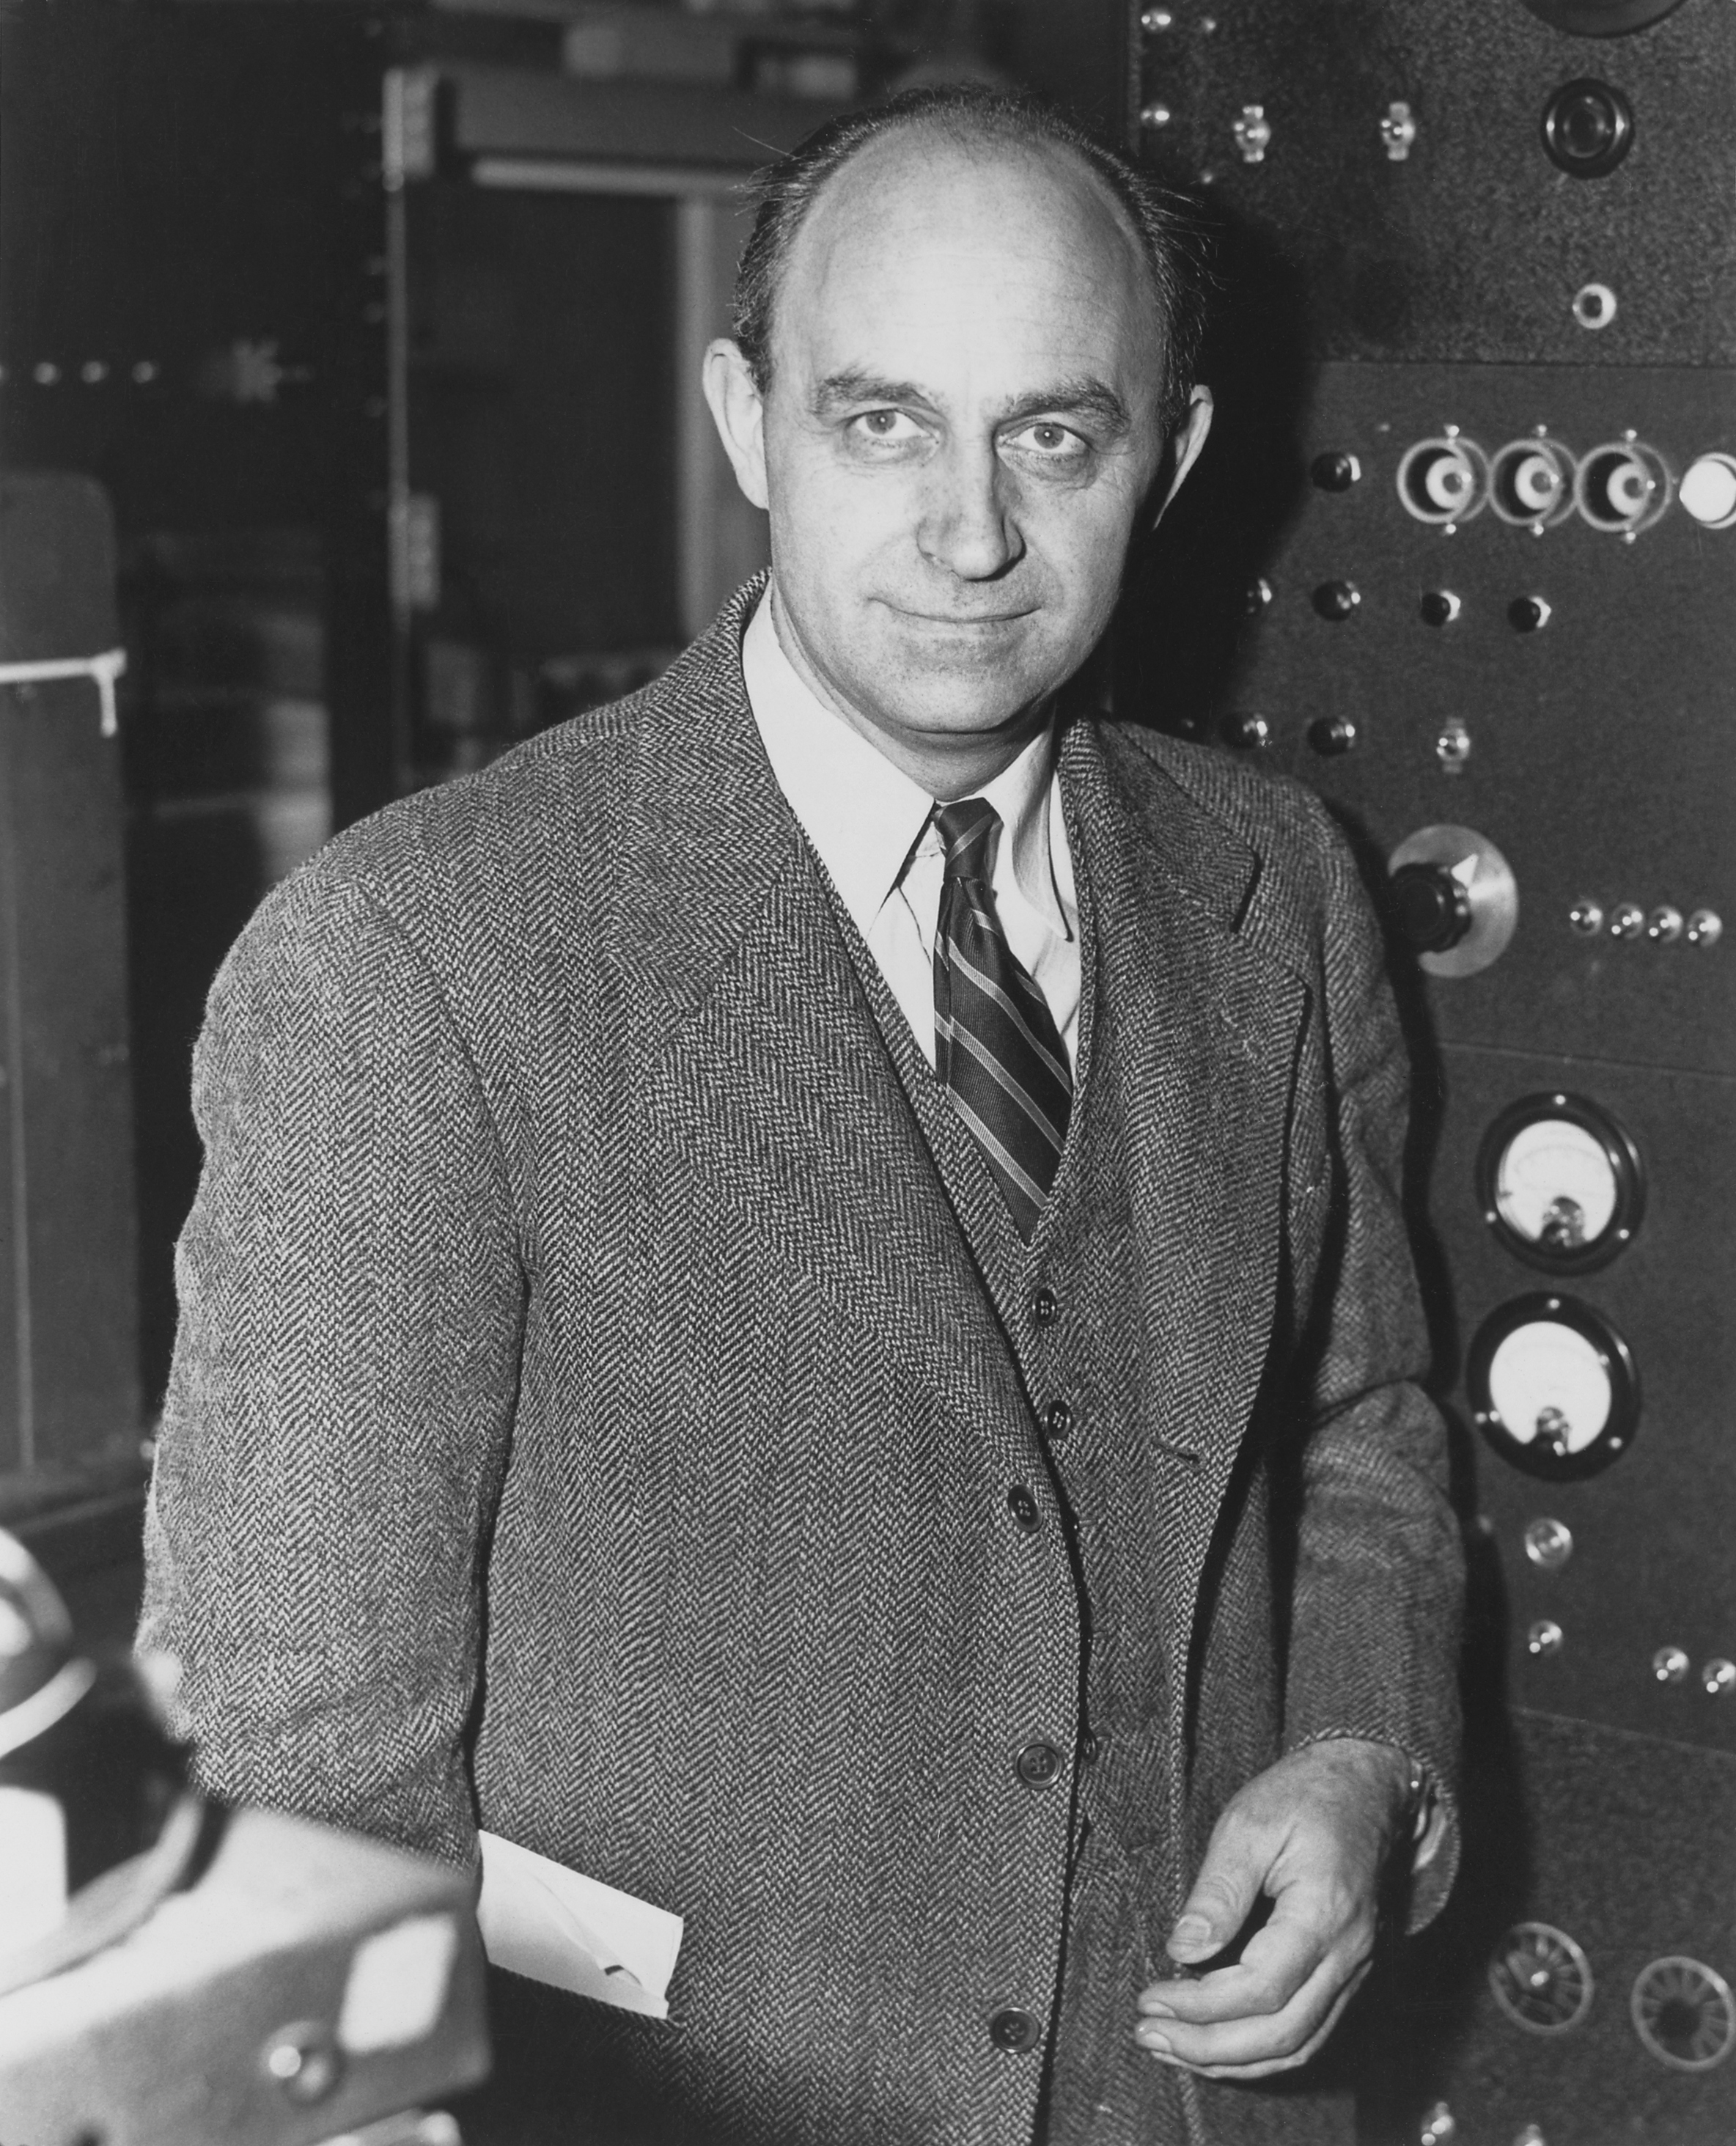
\includegraphics[width=0.4\textwidth, alt={A picture of the Italian-American physicist Enrico Fermi from Wikimedia commons.}]{figures/Enrico_Fermi_1943-49.jpg}
    %}{A picture of the Italian-American physicist Enrico Fermi from Wikimedia commons.}
    \caption{The Italian-American physicist Enrico Fermi from \href{https://commons.wikimedia.org/wiki/File:Enrico_Fermi_1943-49.jpg}{Wikimedia Commons}.}
\end{figure}
\end{center}
While much of physics is about making very precise measurements such as the high energy physics experiments being conducted at CERN, or the measurements of the fundamental constants used to define measurement standards. A lot can be understood by working roughly and making approximations. \\

The standard example of this style of estimation is asking how many piano tuners there are in a certain city. In the lectures we treated the case of London and Ormskirk. This style of approximation problem is often called a \textbf{Fermi Problem} after the physicist Enrico Fermi who liked to ask questions like ``How many piano tuners are there in Chicago?'' Famously Fermi estimated the yield of the first atomic bomb by dropping a scrap of paper and seeing how far it was blown and making some estimates. 

\paragraph{Example 1.1} How many piano tuners are there in London? To answer this start by making a few estimations:
\begin{itemize}
\setlength{\itemsep}{-5pt}
    \item the population of London, around 9 Million people,
    \item how many people have a piano, around 1 in 50,
    \item how often does a piano need tuned, around once a year,
    \item how many pianos can a piano tuner tune in a year, assume 5 a day 230 days a year\footnote{This is potentially the roughest estimate as I know piano tuners who only tune one piano a day, but that is not in a city.}. 
\end{itemize}

Putting this together we then calculate the number of piano tuners as
\begin{align*}
    \text{Number of Piano Tuners} &= \frac{\text{Population of London }}{\text{Number of people per piano} \times \text{Number of tunings a year}}\\
    &=\frac{9\times 10^{6}}{50\times 5\times 230}\simeq 160
\end{align*}

\paragraph{Question 1:}Can you estimate how many piano tuners there are in Ormskirk? Think about how the numbers would change in the above example.\\




\section{The Scientific Method}

In the earlier sections we have alluded to how physics works, constructing a model and then testing it against experiment. This is a very rough description of the \textbf{Scientific Method} which you will meet again in your subject specific modules in semester two and later in your degree. A schematic representation of the scientific method is given in \cref{fig2: scientific method}.
\begin{center}
\begin{figure}[ht]
    %\pdftooltip{
    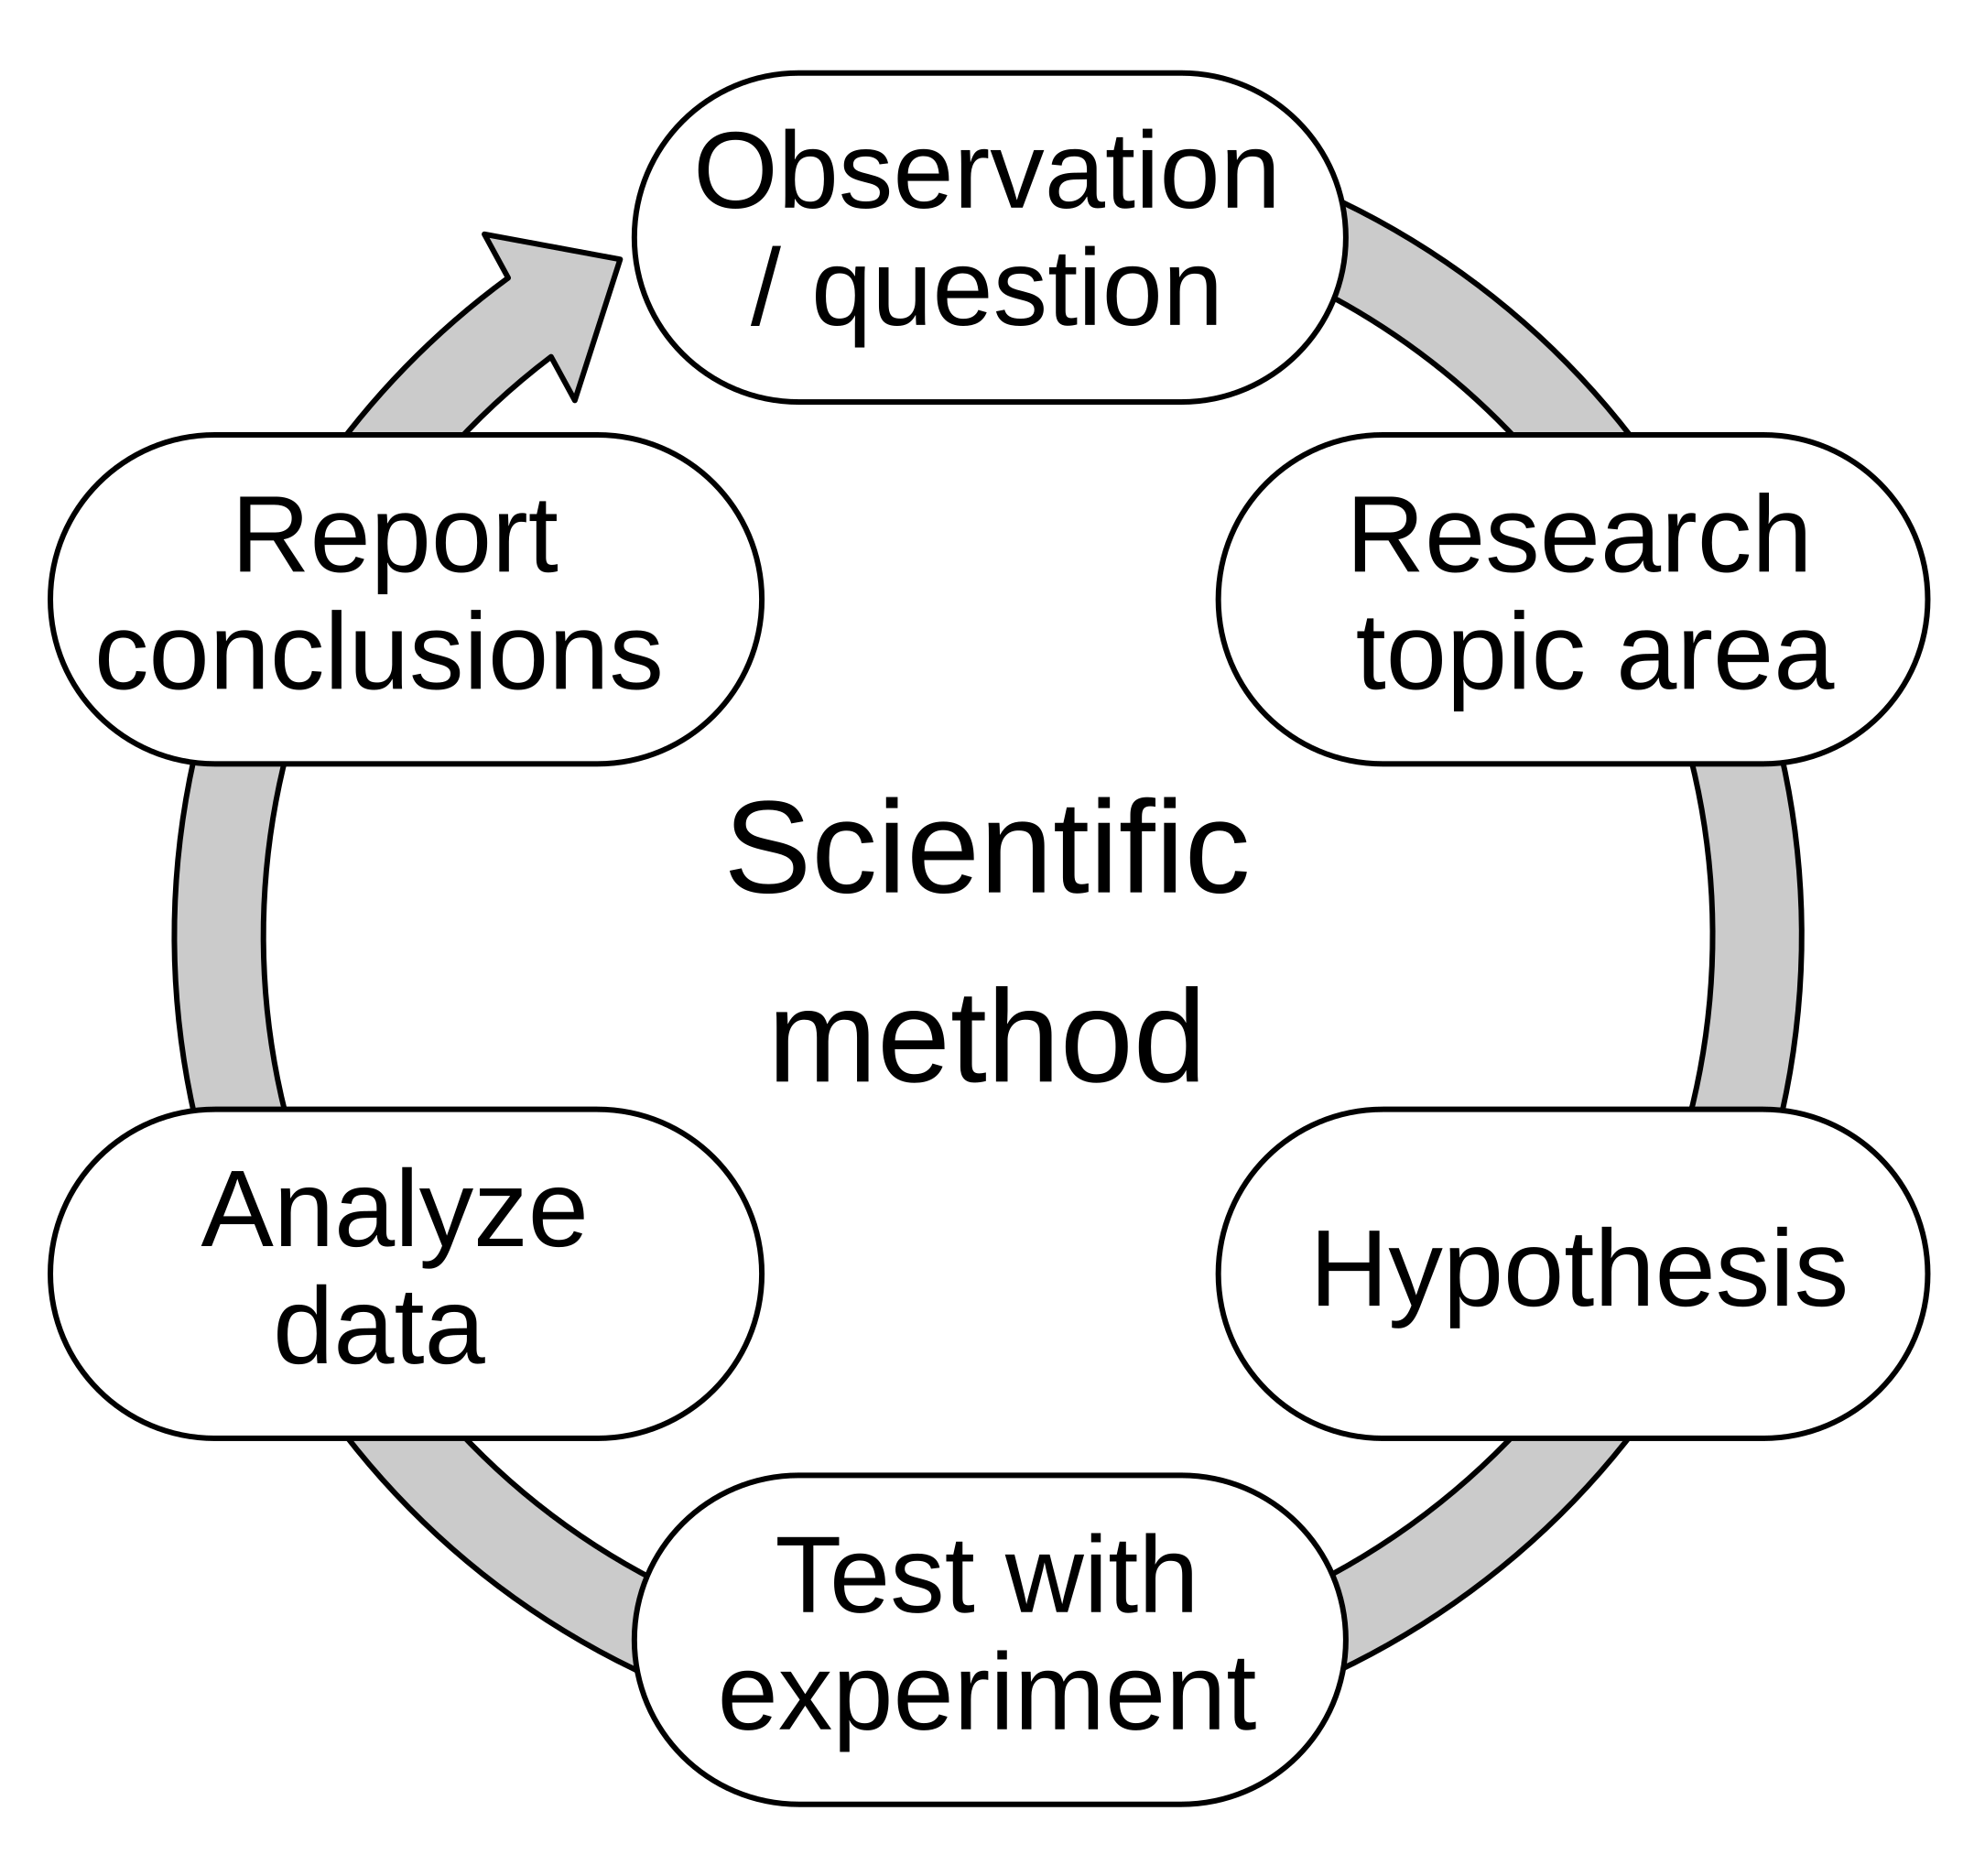
\includegraphics[width=0.6\textwidth,alt={A schematic of the scientific method as a cycle, image from Wikimedia commons.}]{figures/The_Scientific_Method.png}
    %}{A picture showing the scientific method from Wikimedia commons CC BY-SA 4.0 Efbrazil.}
    \caption{A representation of the scientific method from \href{https://commons.wikimedia.org/wiki/File:The_Scientific_Method.svg}{Wikimedia Commons} CC BY-SA 4.0 Efbrazil.}
    \label{fig2: scientific method}
\end{figure}
\end{center}
The process of the scientific method involves three main stages:
\begin{itemize}
\setlength{\itemsep}{-5pt}
    \item Making conjectures (hypothetical explanations) -- these may be mathematical models or just a description of your expectations.
    \item Deriving predictions from the hypotheses as logical consequences -- e.g. think about what your model/ expectations imply will happen.
    \item Carry out experiments or empirical observations based on those predictions -- this means test that reality matches your predictions.
\end{itemize}

This is an empirical method for acquiring knowledge and involves careful observation while applying rigorous scepticism about what is observed. The reason for the scepticism is that you are essentially watching something happen, making a guess why it happens, then testing your guess. It is easy to be biased and think that you have confirmed your guess even if the experiment does not show this. One then formulates a hypothesis, or hypotheses, based on the observations, before refining or eliminating hypotheses based on the experimental findings.\\

Hypotheses enable predictions to be made about outcomes based on observations. A good hypothesis is not just a guess since it can be rigorously tested against an experiment or observation. Hypotheses can be strengthened by using different research methods to carry out and analyse your experiment, e.g. surveys, experiments, statistical analysis, literature review, etc.\\

An effective hypothesis is usually one concise sentence containing the following specific elements:

\begin{itemize}
\setlength{\itemsep}{-5pt}
    \item A prediction:
    \begin{itemize}
\setlength{\itemsep}{-5pt}
    \item An `if/then' statement
    \item A declarative statement
    \item The statement must be what the research is setting out to test
\end{itemize}
    \item Variables:
    \begin{itemize}
\setlength{\itemsep}{-5pt}
    \item Clearly state all the variables that will be considered in the study
    \item Designing an experiment using these variables can prove or disprove the prediction
\end{itemize}
    \item Subject group: 
    \begin{itemize}
\setlength{\itemsep}{-5pt}
    \item State the subjects to be tested during the research
\end{itemize}
\end{itemize}

\paragraph{Example 1.2:}Imagine you are walking in the country side and go past a field with some sheep. If all the sheep that you see are white you may come up with the hypothesis that ``All sheep have white wool''. In this case the subjects are the sheep, the variables are the colour of the wool, and the prediction is that all sheep have white wool. If you keep walking and pass another field where the sheep have multiple colours of wool, say white, brown, and black, then you observe that your hypothesis is false.

\paragraph{Question 2:} How could you refine your hypothesis using the new data that you have taken? Can you tests this refined hypothesis in the same way?\\

During the practical sessions in this module you will carry out experiments, using the scientific method and following the details in the lab manual, and then write up your findings. An important part of scientific writing is putting your work in context and explaining how it connects to the existing literature. To be able to do this you need to build awareness of the existing scientific literature. This may be by looking at the module reading list, reading these lecture notes, looking up the topic online, or any other way to explore what is already known.\\

Remember, science is a continually evolving field; new discoveries and experiments are based on earlier work carried out by other scientists. Any literature that is read and used for inspiration should be referenced by stating how the previous work is related to what you have done. For this module the referencing should be done using the Edge Hill Harvard referencing style, there is information about this on the module's VLE page. \\

When writing up your work you need to be aware that scientific writing is not the same as writing an essay. The key features of scientific writing are: precision, clarity, formal language, and organisation. 

\paragraph{Precision:} Scientific writing relies on unequivocal accuracy, anyone reading it needs to be able to trust what you have written. This means that you need:
\begin{itemize}
\setlength{\itemsep}{-5pt}
    \item \textbf{Objectivity:} take an objective viewpoint towards the subject, the author does not just state their opinion. Relevant facts should be presented, justified, and analysed.
    \item \textbf{Thoroughness:} include as many details as are necessary for readers to thoroughly understand the subject. This is a delicate balance as you should not write too much or it can confuse the reader.
    \item \textbf{Exact language:} the use of figurative or imaginative language should be minimised; words and phrases should be used to convey their literal meaning.
\end{itemize}

\paragraph{Clarity:}A clear and consistent writing style is also important for establishing a trusted voice within the scientific community. It enables others to read your work and replicate any experiments that you have carried out.
\begin{itemize}
\setlength{\itemsep}{-5pt}
    \item The writer should clarify the meaning of any uncommon terms.
    \item The goal of the writing is to clearly explain the work that has been carried out so the results or observations should be summarised in a way that anyone can understand.
    \item The experiment and its results are fully explained.
    \item A consistent system of units are used and this choice is clearly explained. In this module and almost everywhere this choice of units is the SI system.
\end{itemize}

\paragraph{Formal language:}
\begin{itemize}
\setlength{\itemsep}{-5pt}
    \item This maintains professionalism.
    \item Slang and idioms should not be used. Some people also dislike the use of contractions.
    \item Make sure to use proper punctuation and grammar.
    \item The use of common language can help your work appeal to a larger audience. Think about the words and phrases that are used and make sure that they are appropriate, e.g. have you used any synonyms for simple words that could be used instead.
    \item Stick to either British or American English, do not mix words and spellings from the two.
\end{itemize}

\paragraph{Organisation:} Most scientific retaining follows a clear organisational structure. What that structure is depends on the discipline. During this module we will use the following structure:

\begin{itemize}
\setlength{\itemsep}{-5pt}
    \item \textbf{Introduction:}
    \begin{itemize}
\setlength{\itemsep}{-5pt}
    \item Relevant background information required to understand the purpose and findings of the work should be summarised.
    \item The purpose and unique value of the experiment or observation should be explained.
\end{itemize}
    \item \textbf{Materials and methods:}
    \begin{itemize}
\setlength{\itemsep}{-5pt}
    \item Explain how the study or experiment was conducted. e.g. what equipment was used, how did you set it up, describe how you made the measurements.
    \item There needs to be enough detail that someone else could replicate your experiment based on the description.
\end{itemize}
    \item \textbf{Results:}
    \begin{itemize}
\setlength{\itemsep}{-5pt}
    \item Give an objective explanation of the experimental results.
    \item Summarise the relevant quantitative and qualitative data. e.g. use appropriate charts and graphs to display your results.
\end{itemize}
    \item \textbf{Discussion:}
    \begin{itemize}
\setlength{\itemsep}{-5pt}
    \item Give an interpretation of the potential implications of your findings. e.g. how does it compare to your hypothesis or to existing theory. 
    \item Evaluate your results and discuss all of the possible interpretations.
    \item Give an outline for any potential future studies and say what you would do differently, and why, if you were to conduct the experiment again.
    \item Consider potential sources of inaccuracy in your results and talk about why these are present and how they could be minimised.
\end{itemize}
    \item \textbf{Conclusions:} The main points of the report are reiterated and the work is summed up.
\end{itemize}

As part of the assessment for the module you need to write up two of the experiments that you have carried out. The description of the coursework contains an outline of how to structure your work using the organisational style given above.

%%%%%%%%%%%%%%%%%%%%%%%%%%%%%%%%%%%%%%%%%%%%%%%%%%%%%%%%%%%%%%%%%%%%%%%

\chapter{Motion in One Dimension and SUVAT}
\label{sec: motion in 1D}
\section{Mechanics}
Throughout this course we will study objects in motion. This could be a ball rolling down a hill, a spring oscillating up and down, or a pendulum. The first part of this course is focussed on \textbf{kinematics}, the study of how objects move. Later in the module we will also deal with \textbf{dynamics}, the study of why objects move. These are both subsets of \textbf{mechanics}, the study of moving objects. \\


\begin{figure}[ht]
    \centering
    
    {\displaymathother
    \ThisAltText{ This is a diagram of a ball rolling down a hill}
    %\pdftooltip{ 
   \begin{tikzpicture}[line width=1pt,line cap=round,line join=round,x=6mm,y=6mm]
\draw (5,0) arc(0:-90:3) arc(-90:-150:2) arc(30:120:1.5) arc(-60:-120:2) arc(-120:-160:5);
\draw (5,0) arc(180:170:7);
\draw[->,shorten <=7] ({2+2.6*cos(-8)},{2.6*sin(-8)}) arc(-8:-35:2.6);
\draw[green,fill=green!20!white] ({2+2.6*cos(-8)},{2.6*sin(-8)}) circle (0.4);
\end{tikzpicture}
}
   % }{A ball rollling down a hill.}
    \caption{A ball rolling down a hill.}
    \label{fig: ball on a hill}
\end{figure}

Kinematics is concerned with quantities like:
\begin{itemize}
\setlength{\itemsep}{-5pt}
    \item \textbf{Displacement:} The distance an object moves in a given direction, typically measured in metres or similar units.
    \item \textbf{Distance:} How far an object has moved without keeping track of the direction. We use the symbol $s$ for displacement.
    \item \textbf{Speed:} The rate of change of distance with respect to time.
    \item \textbf{Velocity:} The rate of change of displacement with respect to time, e.g. the speed in a given direction. Velocity is usually measured in metres per second, m/s or $\text{ms}^{-1}$. we use the symbols $v$ or $u$ for velocity. When the velocity is constant it is related to the displacement through $v=\frac{s}{t}$, i.e velocity is displacement divided by time.
    \item \textbf{Acceleration:} The rate of change of velocity with respect to time, usually measured in metres per second squared, $\text{m/}\text{s}^{2}$ or $\text{ms}^{-2}$. Acceleration is given the symbol a.
\end{itemize}

The formula relating constant velocity, displacement, and time can be recalled using the formula triangle in \cref{fig: vst triangle}.\\

\begin{figure}[ht]
    \centering
  {\displaymathother
    \ThisAltText{ The formula triangle for displacement, velocity, and time.}
     % \pdftooltip{ 
   \Huge {\formulatriang[.4]{$s$}{}{$v$}{}{$t$}{}}
   }
   %}{The formula triangle for velocity, displacement, and time.}
    \caption{The formula triangle for constant velocity, displacement, and time. To use the triangle cover up the quantity that you want to calculate and you are left with the formula for it. For example if $s$ is covered up we are left with $v\times t$}
    \label{fig: vst triangle}
\end{figure}


Speed and distance are examples of scalars. Quantities that have a size (also called a magnitude) but not a direction. While velocity, displacement, and acceleration are vectors. This means that they have both a size and a direction.\\

The distinction between scalars and vectors is an important one and we will make a lot of use of both quantities repeatedly during this module.



\section{Motion in 1D}
The easiest way to remember the difference is to think about motion along a line in one dimension.\\

\begin{figure}[ht]
    \centering
    %\pdftooltip{
    \ThisAltText{ A one dimensional line signifying the x-axis.}
    \begin{tikzpicture}
\draw[black, ultra thick,->] (-6,0) --(6,0) node[anchor=west]{$x$};
\filldraw[black] (0,0) circle (2pt) node[anchor=south]{0};
\end{tikzpicture}
%}{A schematic of the x-axis }
    \caption{A one dimensional line described by the coordinate x. The point $x=0$ is marked in the middle of the line with $x$ negative to the left of this and positive to the right.}
    \label{fig: x-axis fig}
\end{figure}

The line shown in \cref{fig: x-axis fig} is known as the $x$-axis since the value of $x$ tells us how far along the line we are. In \cref{fig: x-axis fig2} we have two marked points, $x_{1}$ and $x_{2}$ on the $x$-axis. If we think of an object starting at $x_{1}$ and moving to $x_{2}$ then the displacement is the change\footnote{In physics we often use the notation $\Delta$ to mean the change in a quantity.} in position $\Delta x =x_{2}-x_{1}$.\\

The difference between displacement and distance is that the distance is always positive, while the displacement is positive when an object is moving to the right and negative for an object moving to the left.\\

\begin{figure}[ht]
    \centering
    \ThisAltText{ The x-axis with two points marked showing where the object is moving between.}
   % \pdftooltip{
   \begin{tikzpicture}
\draw[black, ultra thick,->] (-6,0) --(6,0) node[anchor=west]{$x$};
\filldraw[black] (-4,0) circle (2pt) node[anchor=south]{$x_{1}$ at $t_{1}$};
\filldraw[black] (4,0) circle (2pt) node[anchor=south]{$x_{2}$ at $t_{2}$};
\end{tikzpicture}
%}{A schematic of the x-axis with two points marked }
    \caption{The $x$-axis with two points marked, $x_{1}$ and $x_{2}$, where the moving object is at the times $t_{1}$ and $t_{2}$.}
    \label{fig: x-axis fig2}
\end{figure}

The \textbf{sign} of $\Delta x$, either positive or negative is the direction, it shows if the object is moving to the right or to the left. Note that the distance the object travels is given by $\vert \Delta x\vert$, the modulus of $\Delta x$.\\

We can explicitly see the difference between distance and displacement if we consider the following two examples:
\begin{itemize}
\setlength{\itemsep}{-5pt}
    \item if $x_{1}=0$ and $x_{2}=2$ then the displacement is $\Delta x=2-0=2$ and the distance is also $2$.
    \item If $x_{1}=0$ and $x_{2}=-2$ then the displacement is $\Delta x = -2-0=-2$ while the distance is still $2$.
\end{itemize}
So the distance does not care whether we move left or right along the $x$-axis, while the displacement cares about the difference.\\

The \textbf{average velocity} is the displacement divided by the difference between the time when the object is at $x_{2}$ and the time at $x_{1}$,
\begin{equation}
    v_{\text{avg}}=\frac{\Delta x}{\Delta t}=\frac{x_{2}-x_{1}}{t_{2}-t_{1}}.
    \label{eq: average velocity}
\end{equation}
You may recognise this as the formula for the gradient of a straight line starting at $(t_{1},x_{1})$ and ending at $(t_{2},x_{2})$. In fact plotting displacement against time is a convenient way to visualise an objects motion. In \cref{fig: displacement time graph 1} we see two examples of this type of plot, in red we have the case of constant velocity, while in blue we see that the velocity is changing.\\

\begin{figure}[ht]
    \centering
    \ThisAltText{ A displacement time graph for constant velocity motion, a straight line, and changing velocity.}
   % \pdftooltip{
   \begin{tikzpicture}
\draw[black, ultra thick,->] (0,0) --(6,0) node[anchor=west]{$t$ axis};
\draw[black, ultra thick,->] (0,0) --(0,6) node[anchor=south]{$x$ axis};
%\draw[step=1cm,gray,very thin] (-2,-2) grid (6,6);
\draw[blue, ultra thick] (0,0) parabola (6,6);
\draw[red, ultra thick, dashed] (0,0) -- (6,6);
% \filldraw[black] (-4,0) circle (2pt) node[anchor=south]{$x_{1}$ at $t_{1}$};
% \filldraw[black] (4,0) circle (2pt) node[anchor=south]{$x_{2}$ at $t_{2}$};
\end{tikzpicture}
%}{A displacement time graph showing the difference between constant velocity motion and motion with a changing velocity.}
    \caption{A displacement time graph showing the difference between constant velocity motion, in red and dashed, and motion with a changing velocity, in blue.}
    \label{fig: displacement time graph 1}
\end{figure}

To read this off the graphs notice that in the constant velocity case no matter which points on the $x$-axis we think of starting and ending at, when we use \cref{eq: average velocity} we will find the same value. This is why we called it the constant velocity case. The velocity is the gradient, rate of change, of a displacement time graph, and a straight line has a constant gradient.\\

For the second case, the blue curve\footnote{Mathematically the blue curve is known as a parabola and is described by a formula $x=t^{2}$ so we can also compute its gradient at any point.}, the gradient is not constant it changes from point to point along the curve. In this case \cref{eq: average velocity} for the average velocity will only be an approximation to the gradient of the curve. This approximation will get better and better as the time difference between the two points, $\Delta t$, gets smaller. To get the instantaneous velocity we would need to take $\Delta t$ to zero, and then the velocity $v$ is given by the \textbf{derivative} of $x$,
\begin{equation*}
    v=\frac{\ud x}{\ud t}.
\end{equation*}
In this module we are not assuming any familiarity with calculus so will not need to use the derivative to calculate the velocity. 

\begin{figure}[ht]
    \centering
    %\pdftooltip{
    \ThisAltText{ A displacement time graph showing an object moving away from its initial position before turning around and returning.}
    \begin{tikzpicture}
\draw[black, ultra thick,->] (0,0) --(7,0) node[anchor=west]{$t$ axis};
\draw[black, ultra thick,->] (0,0) --(0,5) node[anchor=south]{$x$ axis};
%\draw[step=1cm,gray,very thin] (-2,-2) grid (7,7);
\draw[blue, ultra thick] (3,4) parabola (6,0);
\draw[blue, ultra thick] (3,4) parabola (0,0);
% \filldraw[black] (-4,0) circle (2pt) node[anchor=south]{$x_{1}$ at $t_{1}$};
% \filldraw[black] (4,0) circle (2pt) node[anchor=south]{$x_{2}$ at $t_{2}$};
\end{tikzpicture}
%}{A displacement time graph where the object returns to its starting position.}
    \caption{A displacement time graph where the object returns to its starting position. This is the sort of graph we will see when looking at objects falling under gravity next week.}
    \label{fig: displacement time graph 2}
\end{figure}

When the velocity is constant we can just use \cref{eq: average velocity} and the equation triangle in \cref{fig: vst triangle} to relate velocity, displacement, and time. If the velocity is changing in time we need to consider the acceleration. This is easiest to understand if we visualise the changing velocity on a velocity time graph. This is just like the displacement time graphs that we saw above but we plot the velocity of the object on the vertical axis rather than the displacement.\\

\begin{figure}[ht]
    \centering
   % \pdftooltip{
   \ThisAltText{ A velocity time graph showing uniform motion where the velocity follows a straight line.}
   \begin{tikzpicture}
\draw[black, ultra thick,->] (0,0) --(6,0) node[anchor=west]{$t$ axis};
\draw[black, ultra thick,->] (0,0) --(0,6) node[anchor=south]{$v$ axis};
%\draw[step=1cm,gray,very thin] (-2,-2) grid (6,6);
%\draw[blue, ultra thick] (0,0) parabola (6,6);
\draw[blue, ultra thick] (0,2) -- (5,6);
\filldraw[black] (0,2) circle (2pt) node[anchor=east]{$u$};
\filldraw[black] (0,5) circle (2pt) node[anchor=east]{$v$};
\draw[black, ultra thick, dashed] (0,5) --(3.75,5);
\draw[black, ultra thick, dashed] (0,2) --(3.75,2);
\draw[black, ultra thick, dashed] (3.75,0) --(3.75,5);
\filldraw[black] (3.75,0) circle (2pt) node[anchor=north]{$t_{2}=t$};
\filldraw[black] (0,0) circle (2pt) node[anchor=north]{$t_{1}=0\text{s}$};
\end{tikzpicture}
%}{A velocity time graph showing uniform motion.}
    \caption{A velocity time graph showing uniform motion starting with velocity $u$ at time zero and accelerating to have velocity $v$ at time $t_{2}$.}
    \label{fig: velocity time graph 1}
\end{figure}

Consider the motion shown in \cref{fig: velocity time graph 1}, here the moving object has the initial velocity $u$ at time $t_{1}=0\text{s}$ which changes to the final velocity $v$ at time $t_{2}=t$. The acceleration is the rate of change of velocity so the average acceleration is given by
\begin{equation}
    a_{\text{avg}}=\frac{\Delta v}{\Delta t}=\frac{v-u}{t}.
    \label{eq: average acceleration}
\end{equation}

As with velocity, if the acceleration is changing then the instantaneous acceleration will be different from the average acceleration and we would need calculus to compute it properly. In this module we will rarely go beyond the case of constant acceleration\footnote{We will only need this when discussing circular motion later in the module. and there we will describe the acceleration in a slightly different way which avoids using the derivative.}. This is called \textbf{uniform motion}.\\

For uniform motion we can rearrange \cref{eq: average acceleration} to make the final velocity $v$ the subject:
\begin{equation}
    v=u+at.
    \label{eq: Kinematic equation 1}
\end{equation}
This is the first of the so called \textbf{Kinematic equations} that we have met. These are the equations relating velocity, time, acceleration, and displacement, by the end of this module you will be very familiar with using these kinematic equations to solve problems. 

\paragraph{Example 2.1:} A car is travelling at $8\text{m/s}$ and breaks for $6\text{s}$  to reduce its velocity to $2\text{m/s}$ calculate its deceleration.

First collect together what we know about the problem:
\begin{itemize}
\setlength{\itemsep}{-5pt}
    \item initial velocity is $u=8\text{m/s}$
    \item final velocity is $v=2\text{m/s}$
    \item time is $t=6\text{s}$.
\end{itemize}
We know that we are in the realm of uniform motion so can use $a=\frac{v-u}{t}$ to find the acceleration. substituting in the numbers gives:
\begin{align*}
    a&=\frac{v-u}{t}=\frac{2-8}{6}=-\frac{6}{6}=-1\frac{\text{m}}{\text{s}^{2}}.
\end{align*}
The negative sign shows that the car is decelerating and is because the velocity is decreasing. Note that it is very important to always include the units in your final answer.\\

\vspace{2cm}

\section{Kinematic Equations}
There are several other kinematic equations that will be useful, deciding which one to use to solve a given problem is something that you will learn by practising solving problems. In the exam you will be given a formula book that will have most of the equations in it. The formula included in the formula sheet are given at the end of these lecture notes.\\

For completeness we will derive the other kinematic equations here and use them to solve an example. \textbf{You do not need to be able to replicate the derivations, but you do need to know how to use the equations.}\\

The formula above, \cref{eq: average acceleration}, is good if we know any three of initial velocity, final velocity, acceleration, and time. However, often we will be interested in the displacement of an object during its motion. This means that we need a way to calculate displacement in terms of the other quantities.  Let us start with what we know. For an object in uniform motion we have that:
\begin{itemize}
\setlength{\itemsep}{-5pt}
    \item The acceleration is related to the initial velocity, final velocity, and the time the object is moving for through
    \begin{equation*}
        v=u+at.
    \end{equation*}
    \item The displacement of the object at time $t$ is given by
    \begin{equation*}
        s=v_{\text{avg}}t.
    \end{equation*}
    \item The average velocity is given in terms of the initial and final velocity as 
    \begin{equation*}
        v_{\text{avg}}=\frac{v+u}{2}.
    \end{equation*}
\end{itemize}
Substituting $v_{\text{avg}}$ into the expression for the displacement gives
\begin{equation*}
    s=\frac{1}{2}vt+\frac{1}{2}ut,
\end{equation*}
then substitute in \cref{eq: Kinematic equation 1} to get
\begin{equation*}
    s=\frac{1}{2}ut+\frac{1}{2}at^{2}+\frac{1}{2}ut.
\end{equation*}
Grouping the terms together gives the second kinematic equation
\begin{equation}
    s=ut+\frac{1}{2}at^{2}.
    \label{eq: Kinematic equation 2}
\end{equation}
This gives us a relationship between displacement, time, acceleration, and initial velocity.

\paragraph{Example 2.2:} Consider the car from Example 3 which was decelerating. Calculate how far it travels while decelerating. 
First collect what we know:
\begin{itemize}
\setlength{\itemsep}{-5pt}
    \item $u=8\text{m/s}$,
    \item $v=2\text{m/s}$,
    \item $t=6\text{s}$,
    \item $a=-1\text{m/s}^{2}$.
\end{itemize}
We do not need to use $v$ but can substitute the rest into \cref{eq: Kinematic equation 2} to calculate the displacement of the car,
\begin{align*}
    s&=ut+\frac{1}{2}at^{2}\\
     &=8\times 6 +\frac{1}{2}\times \left(-1\right)\times \left(6\right)^{2}\\
     &=48-18\\
     &=30\text{m}.
\end{align*}
So the car travels $30\text{m}$ while decelerating.\\

Next consider the product of acceleration and displacement $as$ and substitute in the expressions that we have for $a$ and $s$:
\begin{align*}
    as  &=\frac{v-u}{t}\times \frac{v+u}{2}t\\
        &=\frac{(v-u)(v+u)}{2}\\
        &=\frac{v^{2}-u^{2}}{2}.
\end{align*}
We rearrange to make $v^{2}$ the subject to give the third kinematic equation
\begin{equation}
    v^{2}=u^{2}+2as.
    \label{eq: Kinematic equation 3}
\end{equation}

\paragraph{Example 2.3:} A car is moving at $120 $km/hr, when the brakes are applied to produce a constant deceleration. After 100 m, the velocity has decreased to 65 km/hr. Find:
\begin{itemize}
\setlength{\itemsep}{-5pt}
    \item[a)] What is the value of the deceleration.
    \item[b)] How long the car was decelerating for
\end{itemize}

As always we start by collecting what we know.
\begin{itemize}
\setlength{\itemsep}{-5pt}
    \item $u=120\text{km/hr}$,
    \item $v=65\text{km/hr}$,
    \item $s=100\text{m}$.
\end{itemize}

For a) we want $a$ but as we do not know $t$ we need to use \cref{eq: Kinematic equation 3} and rearrange it to get
\begin{equation*}
    a=\frac{v^{2}-u^{2}}{2s}=\frac{(65)^{2}-(120)^{2}}{2\times 100}=-50.1\text{km/hr}^{2}.
\end{equation*}
If we convert this to $\text{m/s}^{2}$ we find $a=-0.0039\text{m/s}^{2}$. Again note that the negative sign is because the car is decelerating.\\

b) Now we want the time taken for the the car to travel $100$ m while decelerating. So now we use that the deceleration is constant at $a=-50.1\text{km/hr}^{2}$. This time we will use \cref{eq: Kinematic equation 1} and rearrange to solve for $t$ as
\begin{equation*}
    t=\frac{v-u}{a}=\frac{65-120}{-50.1}=1.098 \text{s}.
\end{equation*}
The are lots of problems for you to practice using the kinematic equations on the tutorial sheets.

%%%%%%%%%%%%%%%%%%%%%%%%%%%%%%%%%%%%%%%%%%%%%%%%%%%%%%%%%%%%%%%%%%%%%%%

\chapter{Freefall and Projectile Motion}

\section{Freefall}
In the last section we talked about motion in one dimension, this can be either horizontal motion, as in all of the examples we studied before, or vertical motion where an object is falling down. This is exactly the problem that Galileo was studying in the 16th century. The apocryphal story is that he was dropping objects of unequal mass off the leaning tower of Pisa and observing that the fell at the same rate. \\

\begin{figure}[ht]
    \centering
    \ThisAltText{ A picture of the Italian polymath Galileio Galilei.}
    %\pdftooltip{
    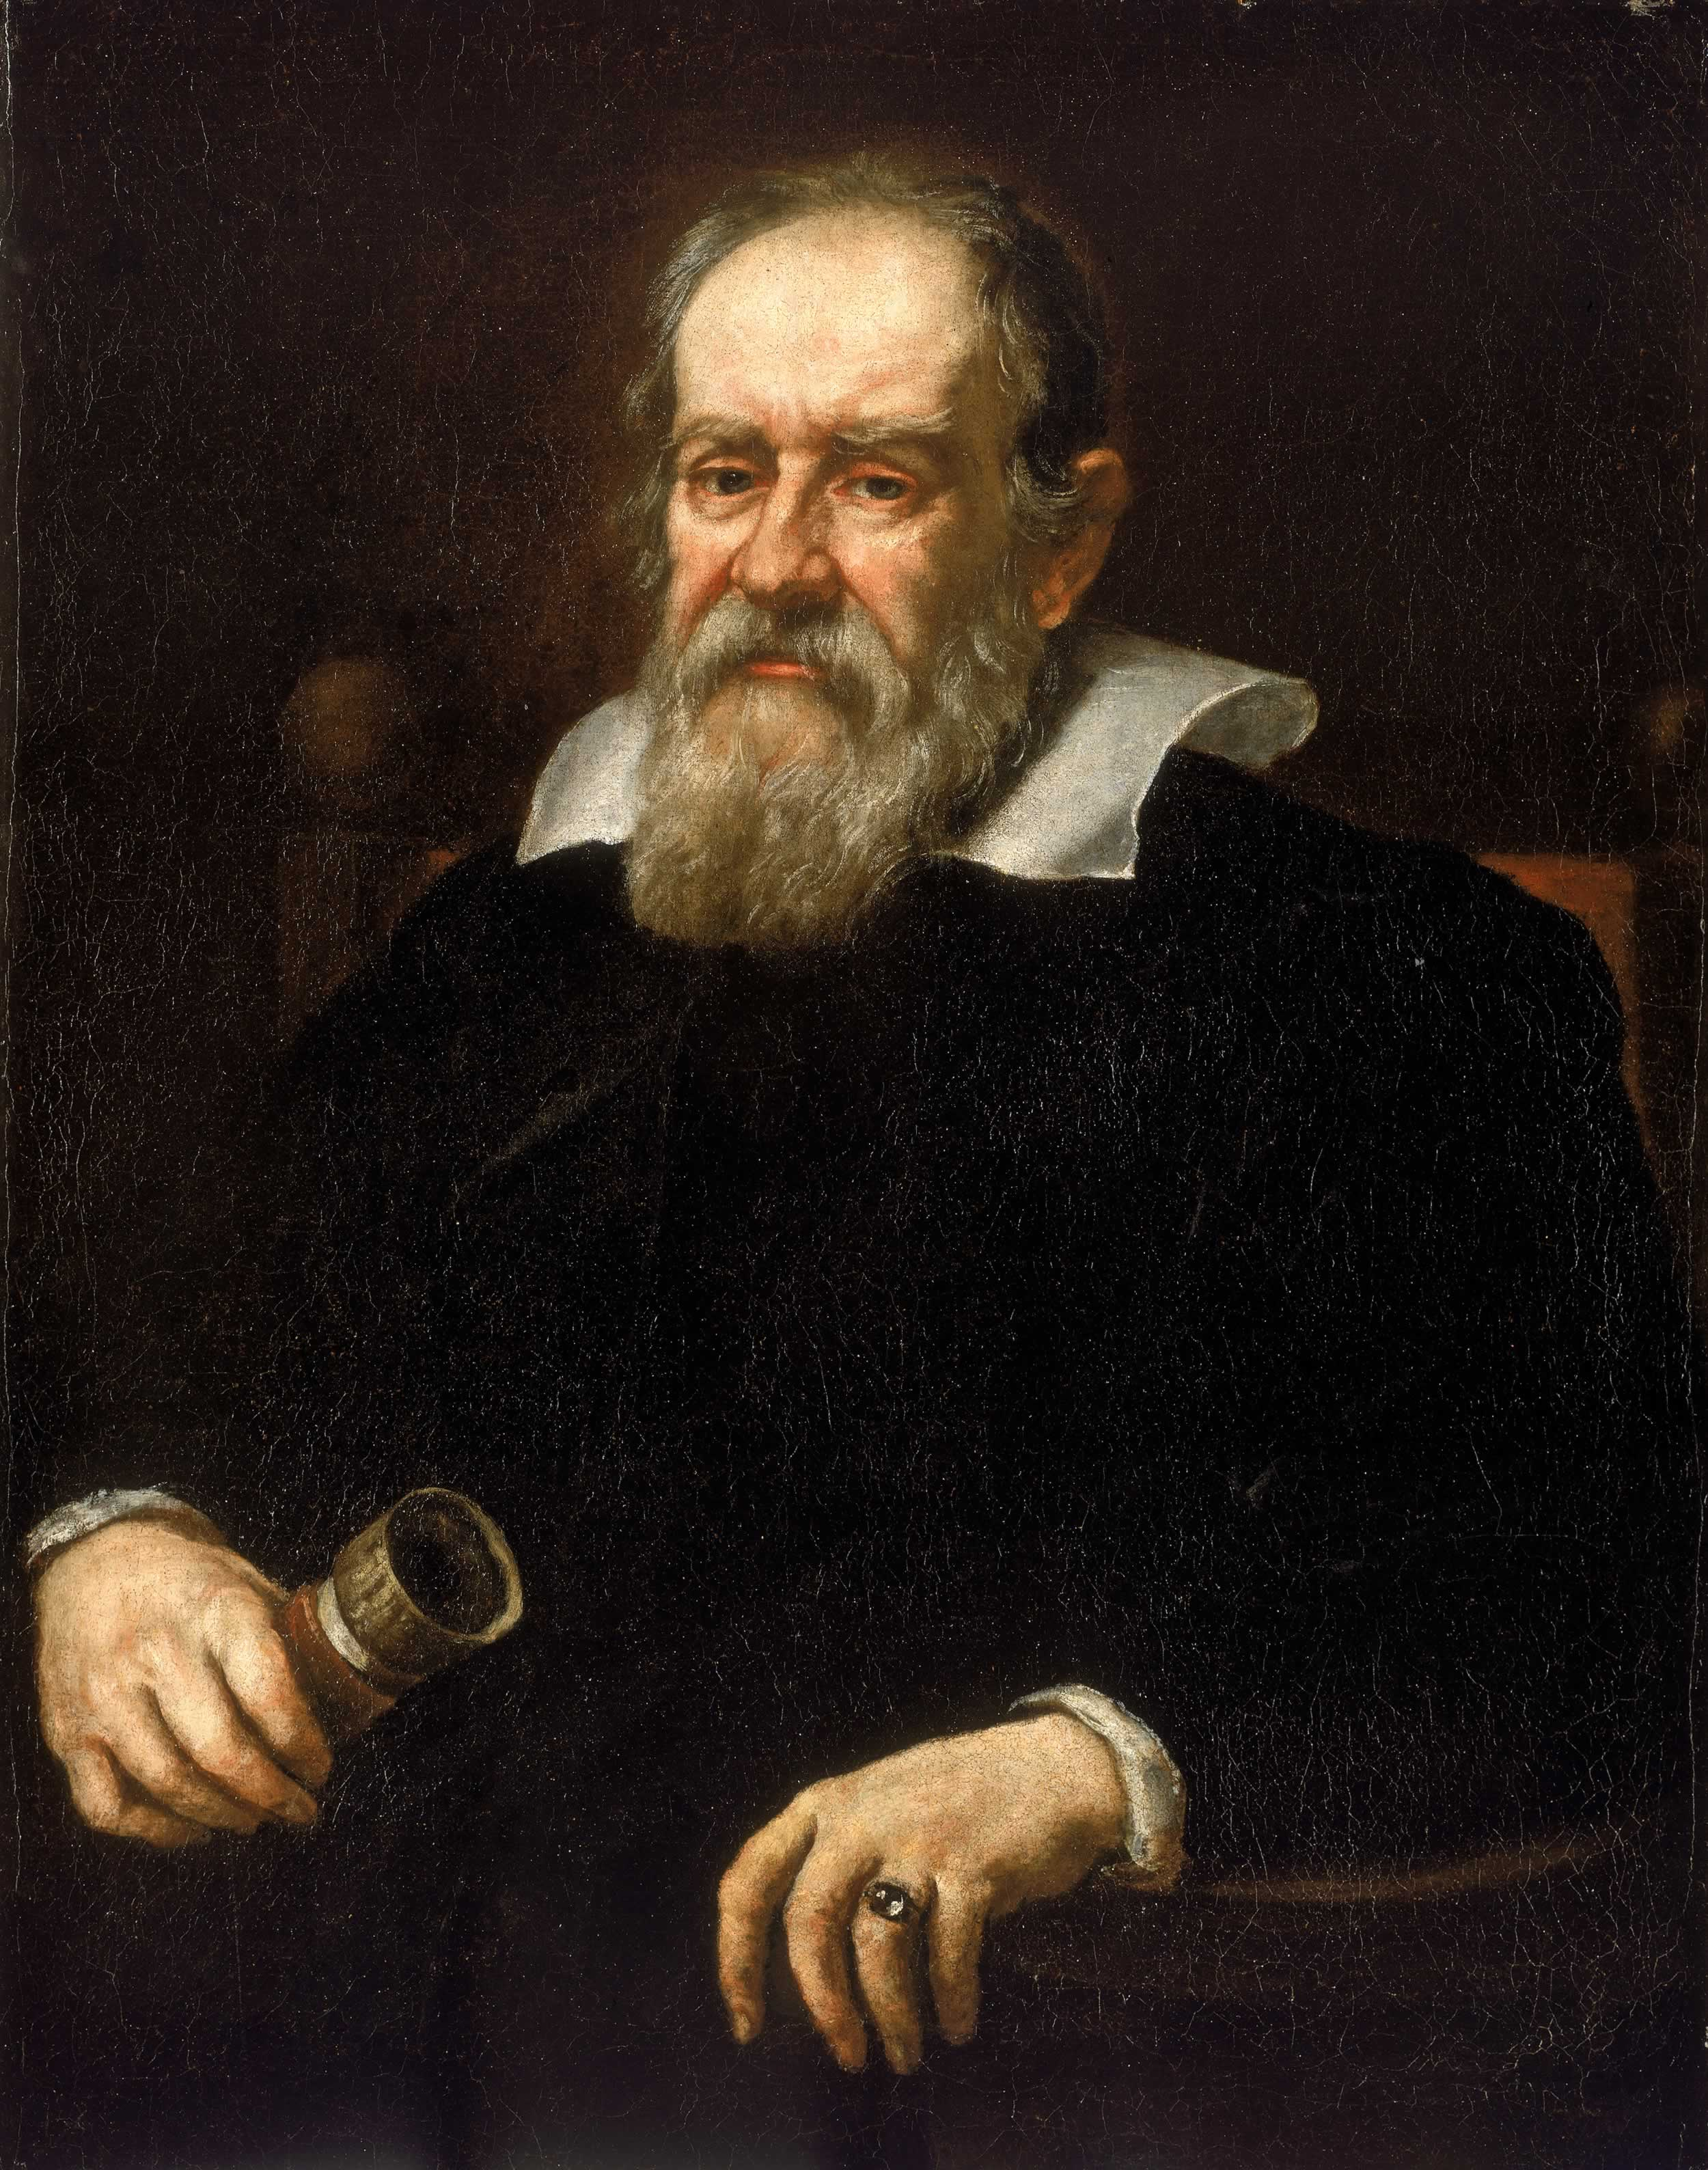
\includegraphics[width=0.4\textwidth]{figures/Galileo.jpg}
    %}{A picture of the Italian polymath Galileio Galilei from Wikimedia commons.}
    \caption{Italian polymath Galileio Galilei, who probably did not drop objects off the leaning tower of Pisa. The image is from \href{https://commons.wikimedia.org/wiki/File:Justus_Sustermans_-_Portrait_of_Galileo_Galilei,_1636.jpg}{Wikimedia Commons}.}
\end{figure}

More precisely Galileo found that (ignoring air resistance) all objects fall at the same rate with their acceleration determined by the gravity acting on the object. This acceleration is known as the \textbf{acceleration due to gravity} $g$ and is approximately constant everywhere on Earth. The value is 
\begin{equation*}
    g=-9.8\text{m/s}^{2}.
\end{equation*}
The minus sign is there because gravity causes objects to accelerate towards the surface of the Earth\footnote{Really they accelerate towards the centre of the Earth but on everyday scales we cannot tell the difference. It also varies with height so if you measure $g$ at the top of a mountain you will get a slightly different answer than if you measure it at sea level, though they will be very close. } and we usually regard upwards as the positive direction.\\

The acceleration due to gravity can be measured by dropping a ball from a known height and timing how long it takes to hit the ground. The second kinematic equation, \cref{eq: Kinematic equation 2} can then be used to solve for the acceleration.  We say that an object only under the influence of gravity is in \textbf{freefall}, as it will keep falling towards the source of gravity until it is stopped by another object, in most cases the surface of the Earth.

\paragraph{Example 3.1:} Consider a coin at rest at the top of a well. If it takes 1.6s to hit the bottom of the well find:
\begin{itemize}
\setlength{\itemsep}{-5pt}
    \item[a)] The depth of the well.
    \item[b)] The speed of the coin just before it hits the bottom of the well.
\end{itemize}

As usual we start by writing down what we know:
\begin{itemize}
\setlength{\itemsep}{-5pt}
    \item $u=0\text{m/s}$ as the coin starts at rest,
    \item $t=1.6\text{s}$,
    \item $a=-9.8\text{m/s}^{2}$ as the coin is falling under gravity.
\end{itemize}

a) We want the depth of the well, this is the displacement of the coin after 1.6s. Use the second kinematic equation and substitute in 
\begin{align*}
    s   &=ut+\frac{1}{2}a t^{2}\\
        &=0 +\frac{1}{2}(-9.8)(1.6)^{2}\\
        &=-12.5\text{m}.
\end{align*}
The minus sign is because this is how far down the coin has fallen and conventionally we think of upwards as the positive direction and downwards as negative.

b) Now we want the final speed of the coin once it has fallen for $1.6$s. Since we know $u,a,$ and $t$, we can use the first kinematic equation to compute this:
\begin{equation*}
    v=u+at =(-9.8)1.6=-15.7\text{m/s}.
\end{equation*}

\section{Vectors}
Now that we have looked at both horizontal and vertical motion it is time to combine them together and study motion in two dimensions. If we wanted to plot displacement against distance in this case we would need to use a three dimensional plot. Usually what is done to visualise the motion is to draw the horizontal and vertical motion separately or to plot horizontal displacement against vertical displacement as in \cref{fig: projectile motion}.\\

\begin{figure}[ht]
    \centering
    %\pdftooltip{
    \ThisAltText{ A plot of projectile motion showing vertical displacement against horizontal displacement.}
    \begin{tikzpicture}
\draw[black, ultra thick,->] (0,0) --(7,0) node[anchor=west]{$x$ axis};
\draw[black, ultra thick,->] (0,0) --(0,5) node[anchor=south]{$y$ axis};
%\draw[step=1cm,gray,very thin] (-2,-2) grid (7,7);
\draw[blue, ultra thick] (3,4) parabola (6,0);
\draw[blue, ultra thick] (3,4) parabola (0,0);
\draw[ultra thick, ->] (0,0) -- (3,4)node[anchor=north]{$\vec{r}$ };
% \filldraw[black] (-4,0) circle (2pt) node[anchor=south]{$x_{1}$ at $t_{1}$};
% \filldraw[black] (4,0) circle (2pt) node[anchor=south]{$x_{2}$ at $t_{2}$};
\end{tikzpicture}
%}{A plot showing projectile motion.}
    \caption{A plot of vertical displacement against horizontal displacement including the vector coordinates of the highest point.}
    \label{fig: projectile motion}
\end{figure}


There are two common, and very closely related, ways to study motion in two, and higher, dimensions:
\begin{itemize}
\setlength{\itemsep}{-5pt}
    \item Study the horizontal and vertical motion separately. This is called working in components and we use the kinematic equations of the previous section but with subscripts on all of the variables to tell us if we are using the horizontal or vertical quantity, e.g. $s_{x}$ for horizontal displacement and $s_{y}$ for vertical displacement or height. 
    \item Work with vectors. 
\end{itemize}

When working in components we write down what we know at the start of a problem separately for the horizontal and vertical cases. e.g. Horizontal motion
    \begin{itemize}
    \setlength{\itemsep}{-5pt}
    \item Initial velocity $u_{x}$.
    \item Final velocity $v_{x}$.
    \item Displacement $s_{x}$.
    \item Acceleration $a_{x}$.
    \item time $t$.
\end{itemize}
Vertical motion
 \begin{itemize}
    \setlength{\itemsep}{-5pt}
    \item Initial velocity $u_{y}$.
    \item Final velocity $v_{y}$.
    \item Displacement $s_{y}$.
    \item Acceleration $a_{y}$.
    \item time $t$.
\end{itemize}
Notice that the time is the same in both cases as we are describing the motion of the same object, just working with the horizontal and vertical pieces separately. If you ever see the words \textbf{neglecting air resistance}, then you can usually assume that $a_{x}=0$ and $a_{y}=g$, that is an object is accelerating vertically due to gravity but is not accelerating horizontally. This is just an approximation but it will serve us fairly well in this module. This is the approach that we will take in the next subsection, and what we will do for most of this course. However, before doing this it is worth having a basic understanding of what is going on with vectors as they will also be important in later weeks when we start discussing forces.\\


\textbf{Vectors} are quantities with both a magnitude and a direction and are usually denoted in either bold or with an arrow on top. For example in \cref{fig: projectile motion} the vector $\vec{r}$ pointing from the origin to the highest point in the objects motion is depicted. The magnitude is the length of the vector and the direction is the angle between the vector and the horizontal axis.\\

\begin{figure}[ht]
    \centering
    \ThisAltText{ A schematic showing how to visualise a vector as a directed line segment.}
    %\pdftooltip{
    \begin{tikzpicture}
\draw[black, ultra thick,->] (0,0) --(7,0) node[anchor=west]{$x$ axis};
\draw[black, ultra thick,->] (0,0) --(0,7) node[anchor=south]{$y$ axis};
\draw[step=1cm,gray,very thin] (0,0) grid (7,7);
\draw[ultra thick, ->] (0,0) -- (3,4)node[anchor=south]{$\vec{r}=\begin{pmatrix}
    x\\ y
\end{pmatrix}$ };
\draw[blue] (1cm,0cm) arc (0:53.13:1cm)node[ anchor=west]{$\theta$};
% \filldraw[black] (-4,0) circle (2pt) node[anchor=south]{$x_{1}$ at $t_{1}$};
% \filldraw[black] (4,0) circle (2pt) node[anchor=south]{$x_{2}$ at $t_{2}$};
\end{tikzpicture}
%}{A plot showing how to visualise a vector}
    \caption{Two ways to visualise a vector.}
    \label{fig: vectors}
\end{figure}

Another way to think of a vector is as a pair $(x,y)$ of a horizontal position and a vertical position, if we thought of putting a grid on a piece of paper as in \cref{fig: vectors} then the pair $(x,y)$ is one way of specifying a point, while the length of a straight line from the point to the origin and the angle $\theta$ between the line and the horizontal is another way to do this. Vectors can be added, subtracted and multiplied. In fact for addition and subtraction there is a nice geometric picture of what is going on as we take the two vectors, place the start of the second one at the end of the first one and see where it ends, the vector sum is then the straight line pointing from the start of the first vector to the end of the second as in \cref{fig: vector addition}. Similarly when subtracting one vector from another we just add the negative of the second vector to the first as shown in \cref{fig: vector subtraction}.\\

\begin{figure}[ht]
    \centering
   % \pdftooltip{
   \ThisAltText{ A schematic of vector addition where the two vectors are lined up nose to tail and the straight line from the tail of the first to the nose of the second is the vector sum of the two.}
    \begin{tikzpicture}
\draw[black, ultra thick,->] (0,0) --(7,0) node[anchor=west]{$x$ axis};
\draw[black, ultra thick,->] (0,0) --(0,7) node[anchor=south]{$y$ axis};
%\draw[step=1cm,gray,very thin] (0,0) grid (7,7);
\draw[ultra thick, ->] (0,0) --node[anchor=south]{$\vec{r}$} (3,4);
\draw[ultra thick, ->] (3,4) --node[anchor=south]{$\vec{s}$} (6,5);
\draw[blue,ultra thick, ->] (0,0) --node[anchor=west]{$\vec{r}+\vec{s}$} (6,5);
% \filldraw[black] (-4,0) circle (2pt) node[anchor=south]{$x_{1}$ at $t_{1}$};
% \filldraw[black] (4,0) circle (2pt) node[anchor=south]{$x_{2}$ at $t_{2}$};
\end{tikzpicture}
%}{vector addition}
    \caption{Vector addition.}
    \label{fig: vector addition}
\end{figure}



\begin{figure}[ht]
    \centering
    %\pdftooltip{
    \ThisAltText{ A schematic of vector subtraction.}
    \begin{tikzpicture}
\draw[black, ultra thick,->] (0,0) --(7,0) node[anchor=west]{$x$ axis};
\draw[black, ultra thick,->] (0,0) --(0,7) node[anchor=south]{$y$ axis};
%\draw[step=1cm,gray,very thin] (0,0) grid (7,7);
\draw[ultra thick, ->] (0,0) --node[anchor=south]{$\vec{r}$} (5,4);
\draw[ultra thick, ->] (5,4) --node[anchor=west]{$\vec{s}$} (6,7);
\draw[red, ultra thick, ->] (5,4) --node[anchor=west]{$-\vec{s}$} (4,1);
\draw[blue,ultra thick, ->] (0,0) --node[anchor=south]{$\vec{r}-\vec{s}$} (4,1);
% \filldraw[black] (-4,0) circle (2pt) node[anchor=south]{$x_{1}$ at $t_{1}$};
% \filldraw[black] (4,0) circle (2pt) node[anchor=south]{$x_{2}$ at $t_{2}$};
\end{tikzpicture}
%}{vector subtraction}
    \caption{Vector subtraction.}
    \label{fig: vector subtraction}
\end{figure}

We said that a vector $\vec{r}$ can be expressed in terms of $x$ and $y$ coordinates as 
\begin{equation*}
    \vec{r}=\begin{pmatrix}
        x\\ y
    \end{pmatrix}.
\end{equation*}
The length or modulus of the vector is given by $\vert \vec{r}\vert =\sqrt{x^2 +y^2}$, and the angle is given by 
\begin{equation*}
    \theta=\arctan\left(\frac{y}{x}\right).
\end{equation*}

We need to be careful which quadrant the vector is in as this formula will always return an angle between $-90^{\circ}$ and $90^{\circ}$, we can tell which quadrant the vector is in by drawing it, to get the correct angle we then need to add or subtract $180^{\circ}$ as is appropriate. This means that when $x$ is negative and $y$ is positive then the angle is $180^{\circ}+\arctan\left(\frac{y}{x}\right)$ and when $x$ and $y$ are both negative the angle is $180^{\circ}-\arctan\left(\frac{y}{x}\right)$. Putting this altogether mathematically gives
\begin{itemize}
\setlength{\itemsep}{-5pt}
    \item $\theta =\arctan\left(\frac{y}{x}\right) $ when $x\geq 0$,
    \item $\theta =180^{\circ}+\arctan\left(\frac{y}{x}\right) $ when$y\geq 0$ and $x<0$,
    \item $\theta =180^{\circ}-\arctan\left(\frac{y}{x}\right) $ when $x,y <0$.
\end{itemize}
Remember that when if we are working in radians then it will be a $\uppi$ that appears instead of $180^{\circ}$.
%\begin{equation*}
%    \theta =\begin{dcases}
%        &\arctan\left(\frac{y}{x}\right) \quad \text{When $x\geq 0$,}\\
%        &180^{\circ}+\arctan\left(\frac{y}{x}\right)\quad \text{when $y\geq 0$ and $x<0$,}\\
%        &180^{\circ}-\arctan\left(\frac{y}{x}\right) \quad \text{When $x,y <0$.}
%    \end{dcases}
%\end{equation*}

Note that when the angle goes beyond $90^{\circ}$ it no longer describes a triangle but the mathematical expressions still make sense. To see why either wait until we discuss circular motion in a later week, or have a look at the mathematical background appendix where a partial explanation of this is given.


\section{Motion in 2D}
We now turn to motion in two dimensions. The most common example of this is \textbf{projectile motion} which is a combination of free fall in the vertical direction and constant speed motion in the horizontal direction.  Projectile motion describes is a good approximation for many things from golf balls and artillery shells, through to thrown stones. We will meet many examples of it in the tutorial problems and in the recommended books. As was mentioned above it is important to start every problem by writing down what we know about the horizontal and vertical motion then identifying what we can compute with that information. This is just like we did with one dimensional motion, but there we did not need to keep track of as many quantities.


\paragraph{Example 3.2:} Consider an arrow fired from the top of a 20 m tower. If the arrow has a horizontal speed of $25 \text{m/s}$, assuming now air resistance find:
\begin{itemize}
\setlength{\itemsep}{-5pt}
    \item[a)] how long the arrow takes to hit the ground,
    \item[b)] the horizontal distance travelled by the arrow\footnote{This is often called the \textbf{range}.}.
\end{itemize}


First write down what we know:

\begin{itemize}
\setlength{\itemsep}{-5pt}
    \item Horizontal:
\begin{itemize}
\setlength{\itemsep}{-5pt}
    \item $t=?$
\item $u_{x}=25\text{m/s}$
\item $v_{x}=u_{x}$, since there is no air resistance we are assuming that $a_{x}=0\text{m/s}^{2}$
\item $s_{x}=?$
\end{itemize}
    \item Vertical:
\begin{itemize}
\setlength{\itemsep}{-5pt}
    \item $t=?$
\item $u_{y}=0\text{m/s}$ as the arrow is fired horizontally
\item $v_{y}=?$
\item $a_{y}=g=-9.8\text{m/s}^{2}$
\item $s_{y}=y=-h=-20m$, this is negative as the arrow will fall $20$m before it hits the ground. 
\end{itemize}
\end{itemize}
a) We want to find the time it takes the arrow to fall $20$ m, this just involves the vertical motion so we can focus on that case and use 
\begin{align*}
s_{y}&=u_{y}t+\frac{1}{2}a_{y}t^{2}\\
&=0+\frac{1}{2}gt^{2},\\
\Rightarrow t&=\sqrt{\frac{2s}{g}}\\
t&=\sqrt{\frac{2\times 20}{9.8}}=2.02 \text{s}.
\end{align*}
If you prefer to rearrange the equation after you have substituted in the numbers then that is ok, just be careful that you do not introduce any rounding errors. Also, note that since the time is always positive we can ignore the negative square root when solving for $t$, if we were solving for a position then we would need to include both\footnote{In the future we will meet examples where $u\neq 0$ and then we have to solve a quadratic equation for $t$ which has two roots, often $t=0$ and another positive value of $t$. }.\\

b) Now we want the horizontal distance travelled and since we know the time that the arrow is in the air for, from part a), and we know that $u_{x}$ is constant, we can use 
\begin{equation*}
s_{x}=u_{x}t=25\times 2.02=50.5\text{m}.
\end{equation*}
So the arrow travel $50.5$ m before it hits the ground.

Often we will be given the velocity in a given direction, and an angle specifying that direction, rather than being given the horizontal and vertical velocities separately. This means that we need to be able to use trigonometry to extract $v_{x}$ and $v_{y}$ from what we are given. See \cref{fig: velocity components} for an example of what this looks like. 
\begin{figure}[ht]
    \centering
    %\pdftooltip{
    \ThisAltText{ A velocity vector decomposed into its horizontal and vertical components.}
    \begin{tikzpicture}[scale=2]
  \coordinate [label=left:$\theta$] (C) at (-1.5cm,-1.cm);
  \coordinate (A) at (1.5cm,-1.0cm);
  \coordinate (B) at (1.5cm,1.0cm);
  \draw (C) -- node[above] {$v$} (B) -- node[right] {$v_{y}$} (A) -- node[below] {$v_{x}$} (C);
  \draw (1.25cm,-1.0cm) rectangle (1.5cm,-0.75cm);
  \tkzMarkAngle[size=1cm,color=blue](A,C,B)
 % \tkzMarkAngle[size=1cm,color=blue](C,B,A)
\end{tikzpicture}
%}{A velocity vector and how it is decomposed into horizontal and vertical components.}
    \caption{A velocity vector and how it is decomposed into horizontal and vertical components.}
    \label{fig: velocity components}
\end{figure}

The key point is that using trigonometry we have that
\begin{align*}
v_{x}&=v\cos\theta,\\
v_{y}&=v\sin\theta.
\end{align*}
There will be lots of opportunity to practice these sorts of problems as well. If you need a reminder about how to use trigonometry then have a look at the appendix on mathematical background or check out some of the links to further reading.

\paragraph{Example 3.3:} Consider an arrow fired at a velocity of $48\text{m/s}$ at an agle of $30^{\circ}$ above the horizontal from a height of $1.5$ m above flat ground. Calculate the maximum height that the arrow reaches, e.g. the peak of the parabola.\\

First we are being asked to find the maximum height, is there anything special about where an object reaches its maximum height? Yes, before the maximum it is going up while after the maximum it is going down, this means that the vertical velocity has changed direction, and it can only do this if it has gone to zero at the maximum height. The maximum height is thus the point where the vertical velocity vanishes, $v_{y}=0$ m/s. In this case we just need to solve a one dimensional problem using the vertical motion. 

We know that:
\begin{itemize}
\setlength{\itemsep}{-5pt}
    \item $t=?$
\item $u_{y}=48\sin\left(30^{\circ}\right)=24\text{m/s}$
\item $v_{y}=0$m/s
\item $a_{y}=g=-9.8\text{m/s}^{2}$
\item $s_{y}=?$
\end{itemize}

Now use
\begin{align*}
v_{y}^{2}&=u_{y}^{2}+2a_{y}s_{y},\\
\Rightarrow s_{y}&=\frac{v_{y}^{2}-u_{y}^{2}}{2a_{y}}\\
&=\frac{0-(24)^{2}}{-2\times 9.8}\\
&=29.3\text{m}
\end{align*}

This is the height the arrow travels from above its starting point, however it starts at $1.5$ m above the ground so attains a maximum height above the ground of $30.8$ m. 

An alternative way to solve this problem would be to use the first kinematic equation, \cref{eq: Kinematic equation 1}, to find $t$ and then substitute this into the second kinematic equation, \cref{eq: Kinematic equation 2}, then solving for $s_{y}$.\\



\paragraph{Example 3.4:} A Batter hits a baseball so that it leaves the bat at a speed of $u=37.0\text{m/s}$ at an angle of $\theta=53.1^{\circ}$. Find:
\begin{itemize}
\setlength{\itemsep}{-5pt}
    \item[a)] The horizontal and vertical components of the velocity at $t=0$ s.
    \item[b)] The position of the ball and its speed after 2s.
    \item[c)] The maximum height reached by the ball and how long it takes to reach this height.
    \item[d)] The range of the ball before it hits the ground.
\end{itemize}
This is a complicated question with several stages, if you can solve this problem then you can solve any of the projectile motion questions that you will come across on the tutorial sheet or on the exam. This brings together everything that we have seen so far.

a) Use trigonometry to calculate the components as
\begin{align*}
u_{x}&=u\cos\theta =37\times \cos53.1^{\circ}=22.2 \text{m/s},\\
u_{y}&=u\sin\theta =37\times \sin53.1^{\circ}=29.6 \text{m/s}.
\end{align*}

b) Let's list what we know and what we do not know:
\begin{itemize}
\setlength{\itemsep}{-5pt}
    \item Horizontal:
\begin{itemize}
\setlength{\itemsep}{-5pt}
    \item $t=2$s
\item $v_{x}=u_{x}=22.2\text{m/s}$ 
\item $s_{x}=?$
\end{itemize}
    \item Vertical:
\begin{itemize}
\setlength{\itemsep}{-5pt}
    \item $t=2$s
\item $u_{y}=29.6\text{m/s}$ as the arrow is fired horizontally
\item $v_{y}=?$
\item $a_{y}=g=-9.8\text{m/s}^{2}$
\item $s_{y}=?$.
\end{itemize}
\end{itemize}
We want both $s_{x}$ and $s_{y}$ so first calculate horizontal then vertical position using kinematic equations:
\begin{align*}
s_{x}&=u_{x}t=22.2\times 2=44.4\text{m},\\
s_{y}&=u_{y}t+\frac{1}{2}a_{y}t^{2}=29.6\times 2+\frac{1}{2}(-9.8)\times 4=39.6\text{m}.
\end{align*}
For the speed we need $v_{y}$ and then can use that the speed is calculated from the velocity as $\text{speed}=\sqrt{v^{2}_{x}+v^{2}_{y}}$. Thus:
\begin{align*}
v_{y}&=u_{y}+a_{y}t=29.6-9.8\times 2=10\text{m/s},\\
\text{speed}&=\sqrt{v^{2}_{x}+v^{2}_{y}}=24.3\text{m/s}.
\end{align*}

c) Now we want to find the maximum height reached by the ball. Recall that $v_{y}=0$ at the maximum height, we can either compute the time using $v_{y}=u_{y}+a_{y}t$ then use this to compute $s_{y}$ through $s_{y}=u_{y}t+\frac{1}{2}a_{y}t^{2}$ or we can use the third kinematic equation, \cref{eq: Kinematic equation 3} to solve for $s_{y}$ directly as
\begin{align*}
v^{2}_{y}&=u^{2}_{y}+2a_{y}s_{y},\\
\Rightarrow s_{y}&=\frac{v^{2}_{y}-u^{2}_{y}}{2a_{y}}\\
s_{y}&=\frac{(29.6)^{2}}{9.8\times 2}= 44.7\text{m}.
\end{align*}

d) Finally, we want to find the range of the ball, that is how far it travels horizontally before hitting the ground. We do this in two steps: 1) find the time it takes the ball to hit the ground by studying the vertical motion, 2) use $t$ and the horizontal motion to find the range.

1) The ground is at $s_{y}=0$ so for the vertical motion we know that:
\begin{itemize}
\setlength{\itemsep}{-5pt}
    \item $t=?$
\item $u_{y}=29.6\text{m/s}$ as the arrow is fired horizontally
\item $v_{y}=?$
\item $a_{y}=g=-9.8\text{m/s}^{2}$
\item $s_{y}=0$m.
\end{itemize}
To find for $t$ we use the second kinematic equation to get a quadratic equation for $t$ that we can then solve:
\begin{align*}
s_{y}&=u_{y}t+\frac{1}{2}a_{y}t^{2}\\
0&=t\left(u_{y}+\frac{1}{2}a_{y}t\right),
\end{align*}
so $t=0$ or $t=-2u_{y}/a_{y}$. Note that getting two values of $t$ makes sense as the ball is at ground level at two times, first when it is hit initially and then when it returns to the ground.  Plugging in the numbers gives that
\begin{equation*}
t=-\frac{2u_{y}}{a_{y}}=\frac{2\times 29.6}{9.8}=6.04\text{s}
\end{equation*}

2) Now that we have $t$ we can solve for $s_{x}$ as
\begin{equation*}
s_{x}=u_{x}t=22.2\times 6.04 =134\text{m}.
\end{equation*}

%%%%%%%%%%%%%%%%%%%%%%%%%%%%%%%%%%%%%%%%%%%%%%%%%%%%%%%%%%%%%%%%%%%%%%%

\chapter{Forces and Momentum}
\section{Force and Motion}
The previous two sections of this module have focussed on kinematics, or how things move, now we turn to \textbf{dynamics}, or why objects move.  Forces are responsible for why objects move. Think of pushing someone on a swing, if you did not give them the initial push they would not start moving. Or think of gravity pulling down on an object, if I let go of an apple it will fall. If an object, or system of objects, changes the state of another, it does so by applying a force. The obvious everyday examples are things that \textbf{push} and \textbf{pull}. \\

Some forces like friction require contact between the objects to act, we call these \textbf{contact forces}. Think of rolling a ball across a table, does it matter what the table is made of? Yes, the rougher the table is the higher its friction and the faster the ball will come to a stop. Other forces, e.g. gravity, magnetism, \dots{}, act over a distance. These are called either \textbf{long range} or \textbf{short range} forces, depending on how long a distance they can act over. \\

Forces are vectors as they have both a magnitude, how strong the effect of the force is, and a direction, which direction the force wants the object to move in.  Since we can have more than one force acting on an object we understand them using a free body diagram as in \cref{fig: free body diagram}. The motion of the object will be governed by the net force, the vector sum, of all the forces acting on the object. This net force is often called the \textbf{resultant}, and the process of finding it is referred to as \textbf{resolving} the forces on the object.\\

Typically when there are more is more than one force acting on an object we use a \textbf{free body diagram} to help us understand the situation. An example free body diagram for an object hanging on the end of a piece of string is given in \cref{fig: free body diagram}.  A free body diagram is not a detailed scale drawing of the problem, it is a diagram depicting a simplified version of the body, all the forces acting on the object as arrows pointing in the direction that they are acting. When solving a problem involving forces it is often a good idea to start with a free body diagram so that you can work out what the net force is.

\begin{center}
\begin{figure}[ht]
\ThisAltText{ A free body diagram showing the forces acting on an object of mass m suspended from a string.}
\def\iangle{35} % Angle of the inclined plane
\def\down{-90}
\def\arcr{0.5cm} % Radius of the arc used to indicate angles
    %\centering
   % \pdftooltip{
   \begin{tikzpicture}[
    force/.style={>=latex,draw=blue,fill=blue},
    axis/.style={densely dashed,gray,font=\small},
    M/.style={rectangle,draw,fill=white,minimum size=0.5cm,thin},
    m/.style={rectangle,draw=black,fill=white,minimum size=0.3cm,thin},
    plane/.style={draw=black,fill=blue!10},
    string/.style={draw=red, thick},
    pulley/.style={thick},]
\node[m] (m) {$m$};
    \draw[axis,->] (m) -- ++(0,2) node[left] {$+$};
    {[force,->]
        \draw (m.north) -- ++(0,1) node[right] {$T$};
        \draw (m.south) -- ++(0,-1) node[right] {$W=mg$};
    };
\end{tikzpicture}
%}{A free body diagram showing the forces acting on an object of mass m.}
    \caption{A free body diagram showing the forces acting on an object of mass $m$ suspended on a string. The weight of the object is pointing down and is given by $W=mg$, and the tension in the string is pointing upwards and is $T$. }
    \label{fig: free body diagram}
\end{figure}
\end{center}

\paragraph{Example 4.1:} Consider an object of weight $\vec{W}$ on an inclined plane, with angle $\theta$. There are three forces acting on the object:
\begin{itemize}
\setlength{\itemsep}{-5pt}
    \item Gravity acts on the objects centre of mass and points straight down to the surface of the Earth. This gives rise to the objects weight $W$.
    \item The object does not fall through the plane due to the support force $S$ acting perpendicular to the plane.
    \item The friction of the plane $F_{r}$ acts on the object, this points upwards along the plane as it is what stops the object from sliding down the plane.
\end{itemize} 

\begin{figure}[ht]
    \centering
   % \pdftooltip{
   \ThisAltText{A picture of a mass on an inclined plane.}
   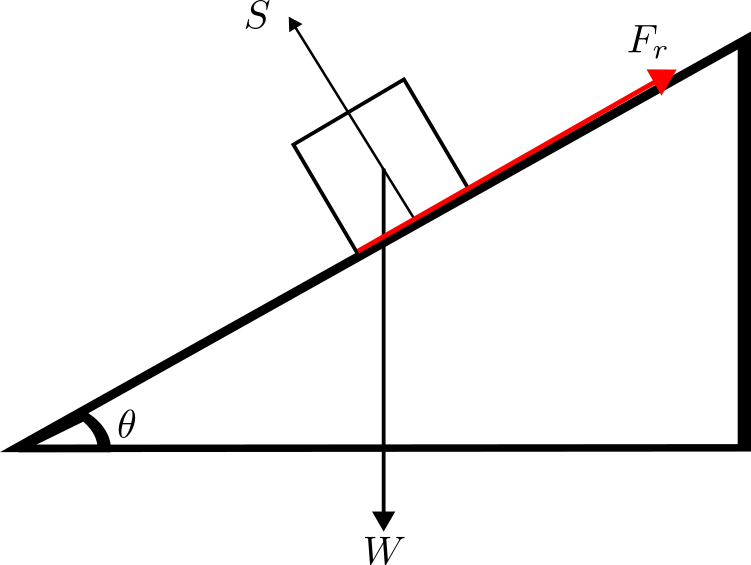
\includegraphics[width=0.4\textwidth]{figures/inclined_plane.png}
   %}{An inclined plane with a mass on it.}
    \caption{An inclined plane with a mass on it. The massive block has three forces acting on it, $W$ its weight pointing straight down, the support force of the plane $S$ acting perpendicular to the plane, and friction $F_{r}$. If this was a free body diagram we would not show the plane and just depict the mass with forces acting on it and the angles that they act at.}
\end{figure}

To understand if the object will move or not we need to resolve the forces and find if there is a net force acting in any direction. If the forces \textbf{balance}\footnote{Here balance means that the resultant vanishes $\vec{W}+\vec{S}+\vec{F}_{r}=\vec{R}=0$.} then the object will be stationary, if they do not balance then the object will slide down the slope. \\


\textbf{Question:} Do you think that whether the object slides down or not depends on the mass of the object or just on the angle of the slope?\\


When the net force $\vec{F}_{\text{net}}$ acting on an object vanishes we say that the object is in \textbf{equilibrium}. Often there is a lot of trigonometry involved in resolving forces so it is a good idea to get a lot of practice doing it.\\

A very common force that we interact with every day is gravity. It acts to attract mass to the centre of the Earth and is responsible for the weight\footnote{Remember that mass and weight are not the same, mass is a scalar quantity that measures the amount of stuff making up an object, while weight is the force of gravity acting on that mass. If you went to the moon where gravity is weaker your mass would be the same but your weight would have decreased.} of an object. For an object of mass $m$, measured in kg, its weight is give by
\begin{equation}
W=mg,
\end{equation}
where $g=-9.8\text{m/s}^{2}$ is the acceleration due to gravity. Remember that the negative sign is there to signify that gravity points downwards. The unit of force is known as the Newton and has the symbol N. \\


To understand how to resolve forces it is best to consider the following example.
\paragraph{Example 4.2:} Consider a $10$kg mass suspended from two pieces of string at angles $70^{\circ}$ and $30^{\circ}$ respectively.  What is the tensions in the strings so that the mass hangs at equilibrium.
\begin{figure}[ht]
    \centering
    %\pdftooltip{
    \ThisAltText{ A mass hanging from two strings at specified angles from the horizontal.}
    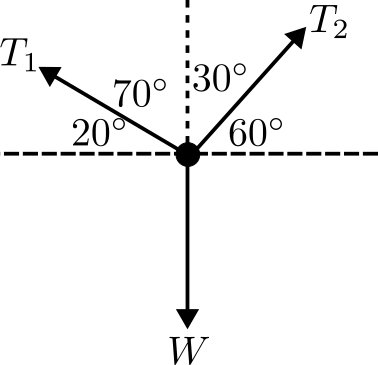
\includegraphics[width=0.3\textwidth]{figures/hanging_mass.png}
    %}{a hanging mass attached to two wires}
    \caption{A $10$ kg mass hanging from two wires.}
    \label{fig: hanging mass}
\end{figure}
\textbf{Tension} is the name for the force in the string pulling the mass upwards, it points along the string.  To understand this problem we can either add together the forces as vectors, or work component wise. In either case, we need to understand the horizontal and vertical components of the vectors.\\

This is easiest for the weight since it only points vertically so the horizontal component vanishes, $W_{x}=0$, and $W_{y}=W$. For the tensions we need to evaluate the components. The angles that we have been given are the angles between the string and the vertical, while we can work with these it is easier to work with the angle between the strings and the horizontal, these are depicted in \cref{fig: hanging mass} as the angles under the string.

\begin{figure}[ht]
    \centering
    %\pdftooltip{
    \ThisAltText{ A triangle showing how to decompose a force into its horizontal and vertical components.}
    \begin{tikzpicture}[scale=2]
  \coordinate [label=left:$60^{\circ}$] (C) at (-1.5cm,-1.cm);
  \coordinate (A) at (1.5cm,-1.0cm);
  \coordinate (B) at (1.5cm,1.0cm);
  \draw (C) -- node[above] {$T_{2}$} (B) -- node[right] {$T_{2y}$} (A) -- node[below] {$T_{2x}$} (C);
  \draw (1.25cm,-1.0cm) rectangle (1.5cm,-0.75cm);
  \tkzMarkAngle[size=1cm,color=blue](A,C,B)
 % \tkzMarkAngle[size=1cm,color=blue](C,B,A)
\end{tikzpicture}
%}{The components of the tension T2.}
    \caption{The components of the tension $T_{2}$.}
    \label{fig: Tension components}
\end{figure}

For $T_{2}$ the horizontal and vertical components are:
\begin{align*}
T_{2x}&=T_{2}\cos(60^{\circ}),\\
T_{2y}&=T_{2}\sin(60^{\circ}).
\end{align*}
Similarly for $T_{1}$ we have:
\begin{align*}
T_{1x}&=-T_{1}\cos(20^{\circ}),\\
T_{1y}&=T_{1}\sin(20^{\circ}),
\end{align*}
where the sign in $T_{1x}$ is there to show that it points to the left.\\

We know that at equilibrium the net force, $F_{\text{net}~}=W+T_{1}+T_{2}$ must vanish, this means that both its horizontal and vertical component must vanish. In other words:
\begin{align}
0&=W+T_{1y}+T_{2y}=W +T_{1}\sin(20^{\circ})+T_{2}\sin(60^{\circ}) \label{eq: vertical force components},\\
0&=T_{1x}+T_{2x}= T_{2}\cos(60^{\circ}) -T_{1}\cos(20^{\circ}) \label{eq: horizontal force components}.
\end{align}
This is a system of equations that we can solve for $T_{1}$ and $T_{2}$. The second equation tells us that 
\begin{align*}
T_{2}=T_{1}\frac{\cos(20^{\circ})}{\cos(60^{\circ})},
\end{align*}
substituting this into the first gives
\begin{align*}
-W=-mg	&=T_{1}\sin(20^{\circ})+T_{2}\sin(60^{\circ})\\
		&=T_{1}\sin(20^{\circ})+T_{1}\frac{\cos(20^{\circ})}{\cos(60^{\circ})}\sin(60^{\circ})\\
		&=T_{1}\left(\sin(20^{\circ})+\frac{\cos(20^{\circ})}{\cos(60^{\circ})}\sin(60^{\circ})\right).
\end{align*}
Now use that $-W=-mg=-10\times (-9.8)=98\text{N}$ and evaluate the trig functions to find:
\begin{align*}
98&=T_{1}\left(0.342+0.866\times\frac{0.9397}{0.5}\right)=1.97T_{1},\\
\Rightarrow T_{1}&=49.8\text{N},\\
T_{2}&=T_{1}\frac{\cos(20^{\circ})}{\cos(60^{\circ})}=49.8\times \frac{0.9397}{0.5}=93.5\text{N}
\end{align*}

Thus the tension in the strings are $T_{1}=49.8$ N and $T_{2}=93.5$N respectively, notice that here we are giving the magnitude of the vector hence both results are positive.\\

There are further examples of resolving forces given in the tutorial problems.

\section{Newton's Laws}
\textbf{Newton's laws}, sometimes referred to as Newton's laws of motion, describe how forces are related to the motion of objects. When you first encounter them they can seem counter intuitive, but they have been very well validated through experiments. There are three laws with each telling us something about how forces cause objects to move.

\begin{figure}[ht]
    \centering
    %\pdftooltip{
    \ThisAltText{ A picture of Sir Isaac Newton from Wikimedia commons.}
    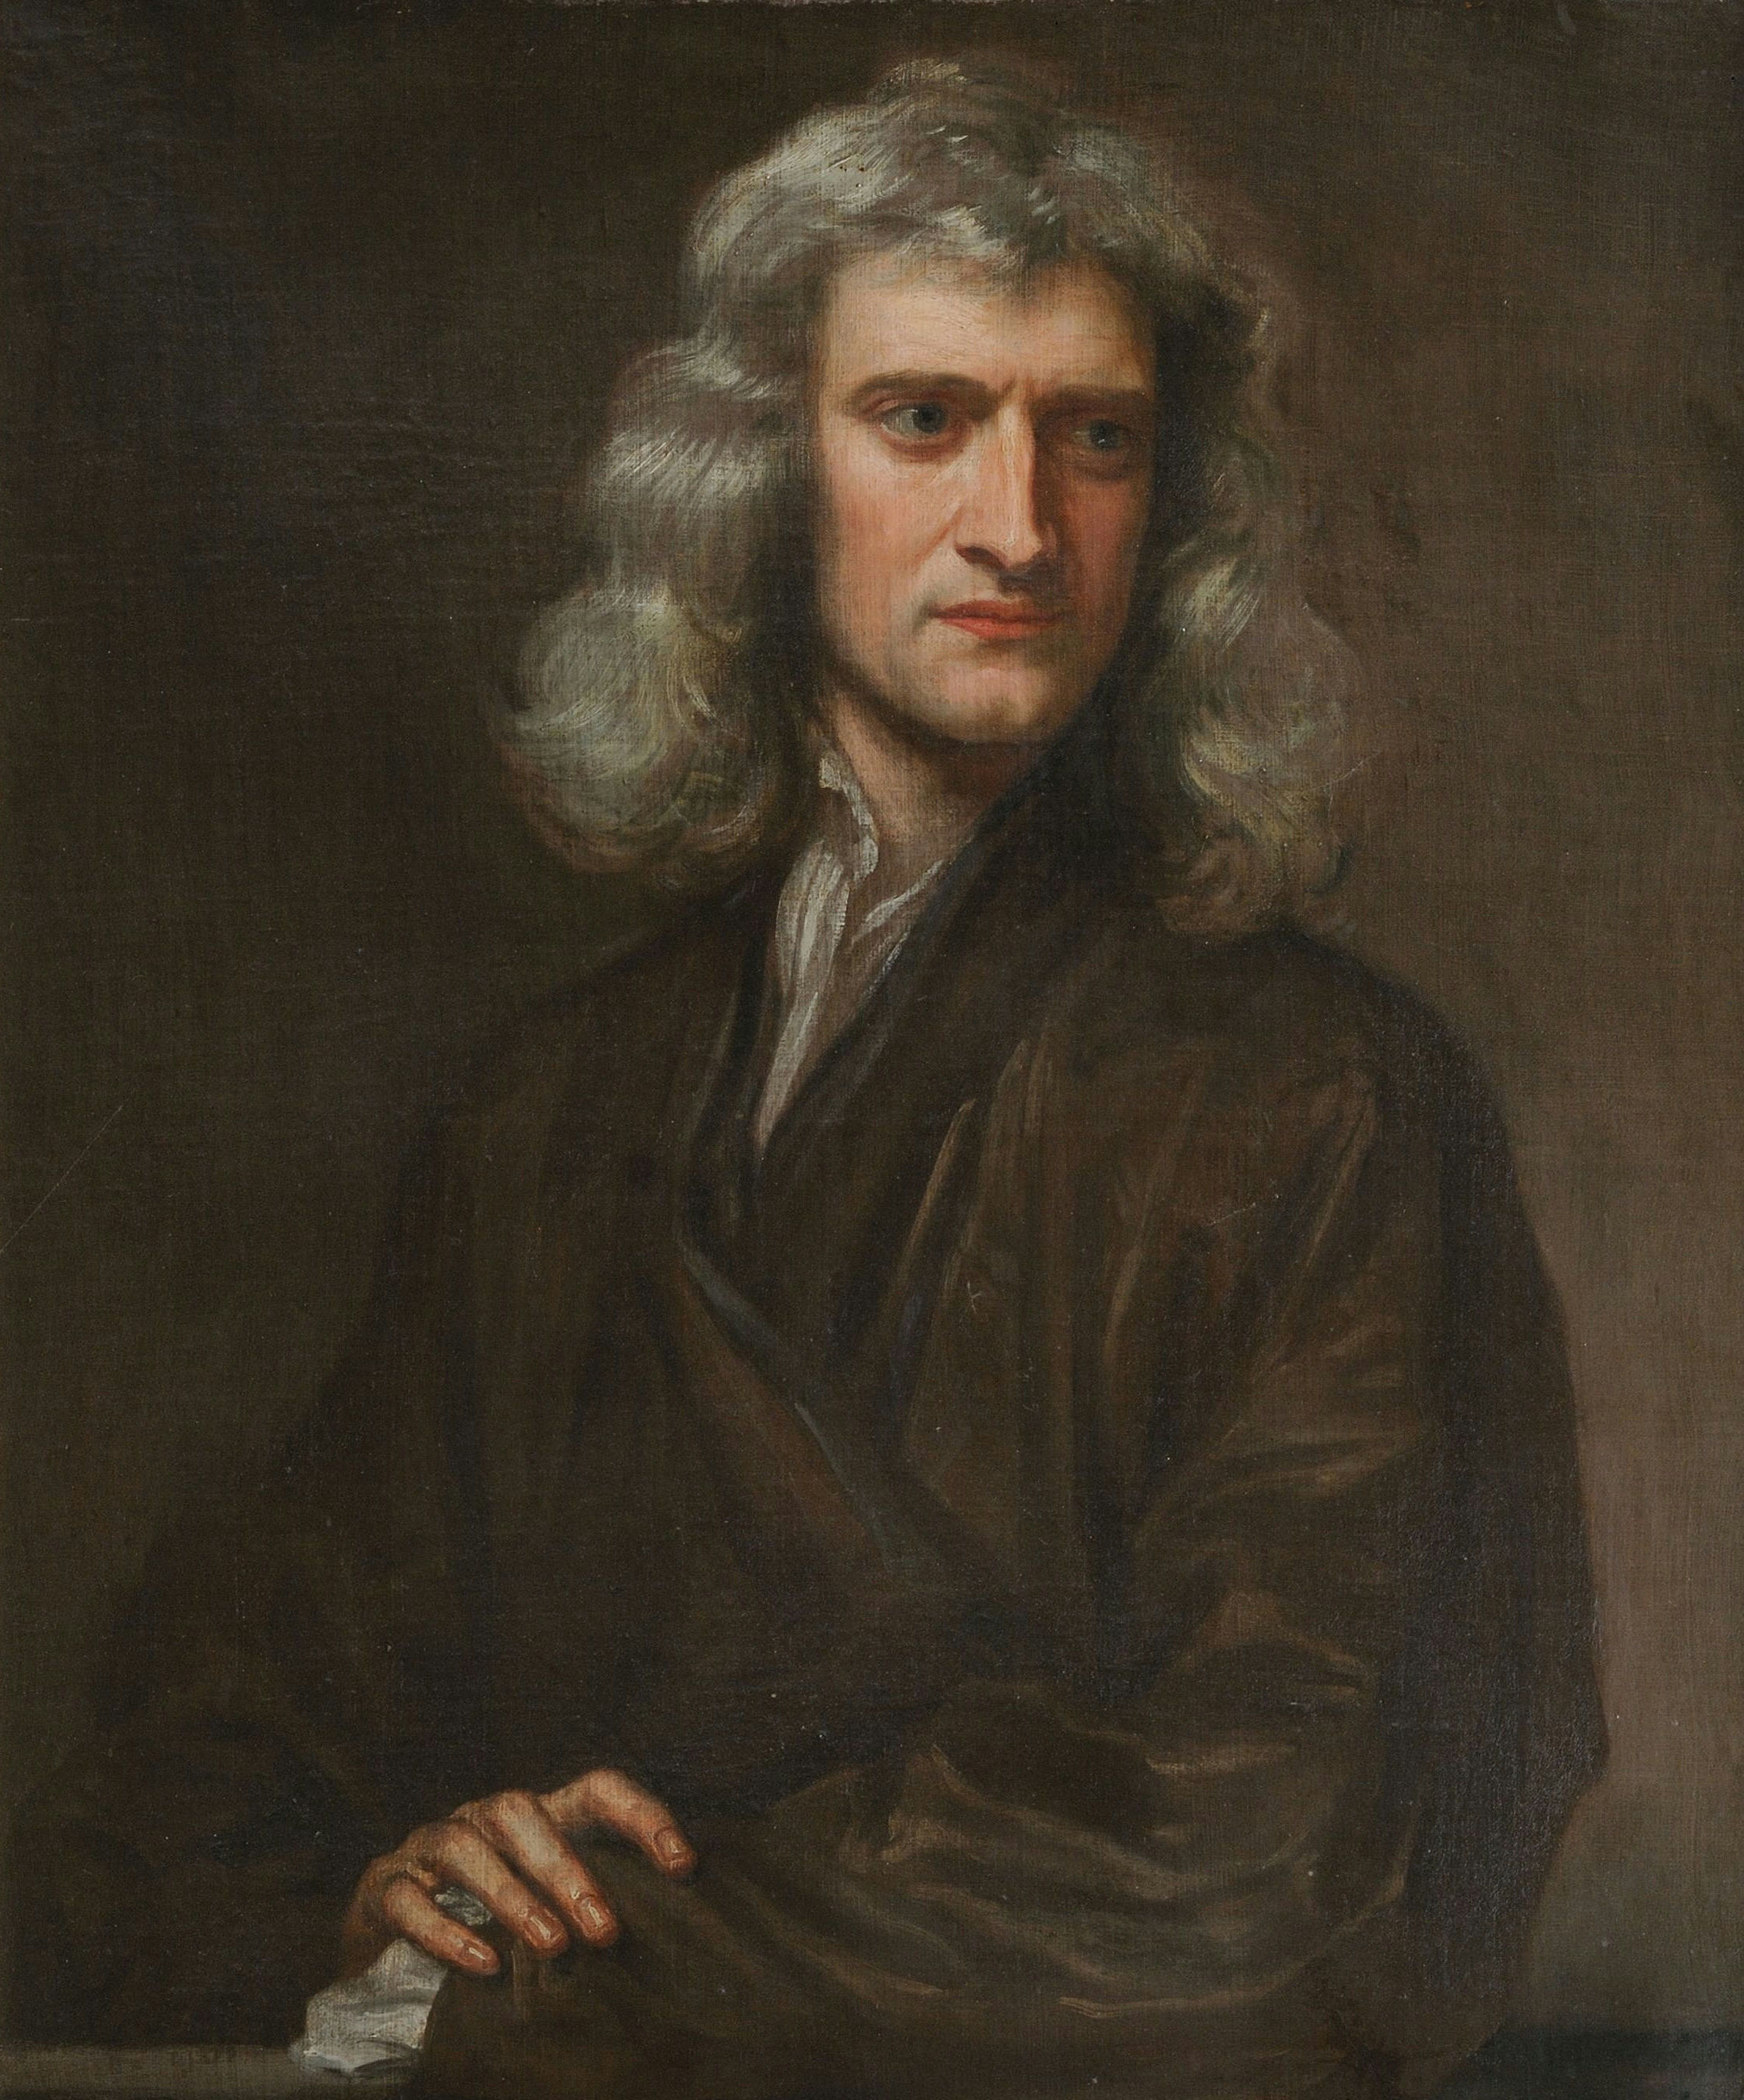
\includegraphics[width=0.4\textwidth]{figures/Portrait_of_Sir_Isaac_Newton,_1689.jpg}
    %}{A picture of the British mathematician and physicist Isaac Newton from Wikimedia commons.}
    \caption{A picture of the British mathematician and physicist Isaac Newton from \href{https://commons.wikimedia.org/wiki/File:Portrait_of_Sir_Isaac_Newton,_1689.jpg}{Wikimedia Commons}.}
\end{figure}

\paragraph{Newton's First Law:} The first law states that a body acted on by \textbf{no} net force moves with constant velocity (which may be zero) and zero acceleration. \\

This is the law that some find counter-intuitive since in everyday experience a ball rolling across a table will not keep rolling forever. However, in this situation there are net forces acting on the ball. There will be friction on the table and air resistance both acting to slow it down.\\

In the absence of friction or drag forces, motion really does persist until a force acts on an object. Think of an air hockey game, you apply an initial force to get the puck moving but after that it keeps travelling at a constant speed until it encounters another force, from the side of the table or the other players paddle. When friction is small we do see behaviour approximating Newton's first law, think of a person on roller skates or in a hover craft.

\paragraph{Newton's Second Law:} If a net external force acts on a body, the body accelerates. The direction of acceleration is the same as the direction of the net force. The mass of the body times its acceleration equals the net force.\\

This statement can look confusing but it is essentially saying that forces cause objects to accelerate and this is described mathematically by
\begin{equation}
\vec{F}_{\text{net}}=m\vec{a}.
\label{eq: N2}
\end{equation}

This is one of the most famous equations in physics and is commonly just referred to as Newton's second law. This equation is how we define the unit of force the Newton, with $1 \text{N}=1\text{kg m/s}^{2}$.  Note that $m\vec{a}$ is not necessarily a force itself, but is the vector sum of all the forces acting on an object. In many of the specific cases that we meet in this module, $F$ will just be one force.

\paragraph{Example 4.3:} Consider a vehicle of mass $600\text{kg}$ accelerating uniformly from rest to a velocity of $8.0\text{m/s}$ in $20$s. Find the force that needs to be applied to achieve this.\\

Recall that the first kinematic equation states that:
\begin{equation*}
a=\frac{v-u}{t}=\frac{8-0}{20}=0.4\text{m/s},
\end{equation*}
thus the force is
\begin{equation*}
F=ma=600\times 0.4=240\text{N}.
\end{equation*}

Newton's second law relies on knowing the mass of the object, but not which mass this is. There are two different definitions of mass in physics, the first is the \textbf{inertial mass}, defined through \cref{eq: N2}, which relates to how ``difficult'' it is to get an object moving. The second definition of mass is the \textbf{gravitational mass} which governs the strength of the gravitational force acting on an object. To the best of our ability to compare these different definitions of mass they agree.\\

What about weight? In everyday usage we use mass and weight interchangeably. However, in physics they are fundamentally different quantities. Mass is an intrinsic property of an object and a scalar quantity, while weight is the force of gravity acting on an object and is a vector. In other words, if the only force acting on an object is gravity, then the acceleration is $a=g$ and Newton's second law says that $mg=F_{W}=W$ is the weight of an object. Sometimes $g$ is referred to as the \textbf{gravitational field strength} as it is not actually constant, it decreases as your height above sea level increases.  The gravitational field strength will also be different on the moon or on a different planet, for example on the moon $g_{\text{moon}}=1.62\text{m/s}^{2}$.

\paragraph{Example 4.4:} Find the constant force needed to accelerate a $200\text{kg}$ mass to $6\text{m/s}$ in $4\text{s}$, neglecting air resistance.\\

First compute the average acceleration through:
\begin{equation*}
a=\frac{v-u}{t}=\frac{6-0}{4}=1.5\text{m/s}^{2},
\end{equation*}
then apply Newton's second law to find
\begin{equation*}
F=ma=200\times 1.5 =300\text{N}.
\end{equation*}

This is just considering the horizontal part of the motion, what about the vertical part? If we drew a free body diagram the vertical forces would be the wight pointing downward and a \textbf{normal reaction} force pointing upwards. The normal force is the support force of the ground acting on the object and stopping the object from falling through the ground. The weight and the normal force must be balanced if the object is not rising and falling. This opens up a new question, what is the normal force? This is where Newton's third law comes in.

\paragraph{Newton's Third Law:} If a body A exerts a force on body $B$ (an \textbf{action}), then body B exerts a force on body A (a \textbf{reaction}). These two forces have the same magnitude but opposite direction. These two forces act on \textbf{different} bodies.\\

Written as an equation this says that
\begin{equation*}
\vec{F}_{\text{A on B}}=-\vec{F}_{\text{B on A}}.
\end{equation*}
Often Newton's third law is expressed as ``Every action has an equal and opposite reaction''.

\paragraph{Example 4.5:} Consider a stationary ball on a table. The net force on the ball is zero since it is stationary and not accelerating. However, there is a \textbf{downward} force on the table from the ball, the weight of the ball. Newton's third law states that the table exerts an \textbf{upwards} force on the ball.\\

Newton's third law applies beyond contact forces, if we drop an apple then both the apple and the Earth accelerate towards each other. This explains the extra support or normal force that is always drawn on free body diagrams, it is the reaction force.\\


\section{Momentum and Collisions}
A closely related concept to force is \textbf{momentum}. It is a vector quantity denoted by $\vec{p}$ and given by the mass times the velocity. As an equation this is given by:
\begin{equation*}
\vec{p}=m\vec{v}.
\label{eq: momentum}
\end{equation*}

Momentum is a useful bookkeeping tool for studying objects in motion because in the absence of external forces the momentum is \textbf{conserved}. This makes it useful in analysing \textbf{collisions} between objects. In practice it is often easier to understand the effects of forces by applying conservation of momentum than by using Newton's second law. There is another conserved quantity that we will use to study motion, the \textbf{energy}. However, mechanical energy is \textbf{not always conserved}, while momentum is. e.g. when we study the collision between two cars, or a meteorite colliding with a planet, momentum is more convenient to use.\\

Momentum is measured in units of $\text{kg m/s}$ as defined through \cref{eq: momentum}.  We can rewritten Newton's second law in terms of the momentum to state that `` The rate of change of the momentum of an object is proportional to the resultant force on it.''

\paragraph{Example 4.6:} Consider an object of mass $m$ travelling at velocity $u$ before being acted on by a constant force $F$ and accelerating to velocity $v$. The initial momentum, before the force acts, is
\begin{equation*}
p_{i}=mu,
\end{equation*}
while the final momentum is 
\begin{equation*}
p_{f}=mv.
\end{equation*}
The change in momentum is thus
\begin{equation*}
\Delta p=p_{f}-p_{i}=mv-mu,
\end{equation*}
this will be positive if the object accelerates and negative if the object decelerates. Using Newton's second law we then get
\begin{equation*}
F=ma=m\frac{v-u}{t}=\frac{mv-mu}{t}=\frac{\Delta p}{t}.
\end{equation*}
This is a convenient rewriting of Newton's second law where $F$ is the force acting the object, $t$ is the length of time that the force is acting for, and $\Delta p$ is the change of momentum due to the force.

In general we will write the change of momentum as either $\Delta p$ or $\Delta \left(mv\right)$. The change in momentum is often referred to as the \textbf{impulse} and we saw above that it is given by the force multiplied by the time that the force acts over, $J=F t$. The example that we gave above had $m$ kept constant, however the mass can also change. This means that we should really write Newton's second law as
\begin{equation*}
F=\frac{\Delta\left(mv\right)}{\Delta t}.
\end{equation*}

If the mass changes at a constant rate but the velocity is constant then the force is 
\begin{align*}
F=v\frac{\Delta m}{\Delta t},
\end{align*}
that is the force depends on the change of mass per second.

\paragraph{Example 4.7:} The case of changing mass is important when studying rockets. A rocket ejects its burnt fuel at a constant speed. Then $v$ is the speed that the hot gas is expelled from the engine and $\Delta m/\Delta t$ is the mass of hot gas lost per second.  A nice discussion of the physics of the rocket equation is given in this \href{https://www.youtube.com/watch?v=V_brZ-KWY3g}{YouTube} video. Though be careful as a different sign convention is in the YouTube video.

\paragraph{Example 4.8:} Consider an object of mass $50 \text{kg}$ which is initially at rest before being acted on by a $10\text{N}$ force for $20\text{s}$. Find:
\begin{itemize}
\setlength{\itemsep}{-5pt}
    \item[a)] The change in momentum
    \item[b)] The velocity of the object after the force has acted.
\end{itemize} 

a) We know that 
\begin{align*}
F&=\frac{\Delta p}{\Delta t}\\
\Rightarrow \Delta p&=F\Delta t\\
&=10\times 20 =200 \text{Ns}.
\end{align*}

b) Now we now that the initial momentum is $p_{i}=0\text{kgm/s}$ and that at $20\text{s}$ the final momentum is $p_{f}=200\text{kgm/s}$. The velocity is thus
\begin{equation*}
v=\frac{p}{m}=\frac{200}{50}=4\text{m/s}.
\end{equation*}

From our everyday experience, we know that the harder we hit a ball the further it will travel. The impact changes the momentum over a very short time. We call the force associated with the change in momentum an \textbf{impact force},
\begin{equation*}
F=\frac{\Delta\left(mv\right)}{t}.
\end{equation*}

\paragraph{Example 4.9:} Consider a ball of mass $m=0.63\text{kg}$, initially at rest, which is struck by a bat and accelerated to a velocity of $35\text{m/s}$. The  contact time between the ball and the bat is $25\text{ms}$. Find:
\begin{itemize}
\setlength{\itemsep}{-5pt}
    \item[a)] The momentum gained by the ball.
    \item[b)] The average force acting on the ball.
\end{itemize} 
As in kinematics problem we start by writing down what we know and do not know about the initial and final configuration:
\begin{itemize}
\setlength{\itemsep}{-5pt}
    \item Initial:
    \begin{itemize}
\setlength{\itemsep}{-5pt}
    \item $t=0\text{s}$
    \item $u=0\text{m/s}$
    \item $p_{i}=mu=0\text{kgm/s}$
\end{itemize} 
    \item Final:
    \begin{itemize}
\setlength{\itemsep}{-5pt}
    \item $t=25\text{ms}$
    \item $v=35\text{m/s}$
    \item $p_{f}=?$
\end{itemize} 
\end{itemize} 
a) Calculate the change in momentum by finding the final momentum
\begin{equation*}
p_{f}=mv=0.63\times 35 =22\text{kgm/s}.
\end{equation*}

b) The impact force is
\begin{equation*}
F=\frac{\Delta p}{t}=\frac{22}{0.025}=880\text{N}.
\end{equation*}


Often it can be useful to plot force against time for an impact force. Typically we will find that the force acts over a very short time and can be quite sharply peaked. The average force of impact is the area under this curve.\\

\vspace{2cm}

\section{Impact and Conservation of Momentum}
Recall that momentum us a vector so when a ball bounces off a wall and rebound its momentum will change direction.  This is shown in \cref{fig: recoiling ball}. After a normal collision the ball rebounds and the direction of momentum is reversed. If we calculate $\Delta p$ we find that
\begin{equation*}
\Delta p=m(-u)-mu=-2mu,
\end{equation*}
this is with the sign convention that towards the wall is positive and away from the wall is negative.

\begin{figure}[ht]
    \centering
    \ThisAltText{A ball bouncing off a wall and reflected backwards with the velocity flipping its sign..}
    %\pdftooltip{
    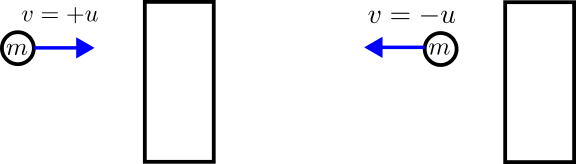
\includegraphics[width=0.4\textwidth]{figures/recoil.png}
    %}{A ball recoiling off a wall}
    \caption{A ball recoiling off a wall, the velocity afterwards is the negative of the velocity before.}
    \label{fig: recoiling ball}
\end{figure}

For an oblique impact we need to take account of the angle of incidence of the object on the wall -- done properly factors of $\cos\theta$ will show up when we work out what the initial and final momentum are. What we need to know is that the angle the ball comes in at will be equal to the angle it comes out at.

\paragraph{Example 4.10:} A tennis ball of mass $0.2\text{kg}$ moving at a speed of $18\text{m/s}$ is hit by a racket causing it to go back in the direction that it came from at a speed of $15\text{m/s}$. Given that the contact time is $0.12\text{s}$ find:
\begin{itemize}
\setlength{\itemsep}{-5pt}
    \item[a)] The change in momentum of the ball.
    \item[b)] The impact force on the ball.
\end{itemize} 
a) We know that $m=0.2\text{kg}$, $u=+18\text{m/s}$, and $v=-15\text{m/s}$, so 
\begin{equation*}
\Delta p=mv-mu=0.2\times(-15)-0.2\times 18=-6.6\text{kgm/s}.
\end{equation*}

b) Impact force is
\begin{equation*}
F=\frac{\Delta}{t}=-\frac{6.6}{0.12}=-55\text{N}.
\end{equation*}

An important principle when analysing impact forces and collisions is the \textbf{conservation of momentum}. This states that ``for a system of interacting objects, the total momentum remains constant provided no external resultant force acts on the system.''\\

Consider two objects which collide with each other then separate. The momentum of each object changes, but they exert equal and opposite forces on each other, by Newton's third law, so the total momentum is unchanged. In other words, the change in momentum of one object is equal and opposite to the change in momentum of the other object. \\

To see this in action consider two billiard balls $A$ and $B$ which collide and then separate. The impact force from $B$ on $A$ changes the velocity of $A$ from $u_{A}$ to $v_{A}$ in the contact time $t$. This force is
\begin{equation*}
F_{1}=\frac{m_{A}v_{A}-m_{A}u_{A}}{t},
\end{equation*}
by analogy
\begin{equation*}
F_{2}=\frac{m_{B}v_{B}-m_{B}u_{B}}{t}.
\end{equation*}

From Newton's third law these forces are equal and opposite so $F_{1}=-F_{2}$, which means that
\begin{equation*}
\frac{m_{A}v_{A}-m_{A}u_{A}}{t}=-\frac{m_{B}v_{B}-m_{B}u_{B}}{t},
\end{equation*}
which rearranges to

\begin{equation*}
m_{A}u_{A}+m_{B}u_{B}=m_{A}v_{A}+m_{B}v_{B}.
\end{equation*}

We often write this as in terms of the momentum as
\begin{equation}
p_{i}=p_{f}
\label{eq: conservation of momentum}
\end{equation}

\paragraph{Example 4.11:} A wagon $A$ of mass $4500\text{kg}$ is moving along a level track at a speed of $3\text{m/s}$ when it collides with and couples to a second wagon $B$ of mass $3000\text{kg}$ which is initially stationary. Calculate the velocity of the two wagons after the collision.\\

Note that since the objects stick together after the collision, the conservation of momentum becomes
\begin{equation*}
m_{A}u_{A}+m_{B}u_{B}=(m_{A}+m_{B})v_{f}.
\end{equation*}

The initial momentum is
\begin{equation*}
p_{i}=m_{A}u_{A}+m_{B}u_{B}=4500\times 3+3000\times 0=13500\text{kgm/s}.
\end{equation*}
The final momentum is
\begin{equation*}
p_{f}=v_{f}(4500+3000) \text{kg} =v_{f}\times 7500\text{kg}.
\end{equation*}
Conservation of momentum then implies that
\begin{align*}
v_{f}\times 7500\text{kg}&=13500\text{kgm/s}\\
v_{f}&=\frac{13500}{7500}\text{m/s}=1.8\text{m/s}.
\end{align*}

In the next section we will meet another quantity that we can also use to study objects in motion, and more generally. The \textbf{energy}.  While momentum is always conserved, in the absence of net external forces, mechanical energy is not. This leads us to distinguish between two different types of collisions: \textbf{elastic collisions} where both are conserved, and \textbf{inelastic collisions} where momentum is conserved but mechanical energy is not. Here \textbf{mechanical energy} means the kinetic energy or energy of motion. You can practice using the conservation of momentum by solving some of the problems on the tutorial sheet.


%%%%%%%%%%%%%%%%%%%%%%%%%%%%%%%%%%%%%%%%%%%%%%%%%%%%%%%%%%%%%%%%%%%%%%%

\chapter{Work and Energy}
\label{sec: work and energy}

\section{Forces and Work}
In principle using the contents of the previous sections, Newton's laws, momentum, and the kinematic equations, we can solve pretty much any problem in mechanics. However, Newton's laws are not always easy to apply. We say before that working with momentum gave us one way to study objects in motion without using Newton's laws directly. Another approach is to think in terms of \textbf{work} and \textbf{energy}.\\

Energy is another quantity that is conserved, though it can change form so the energy of a given type is not conserved as we will see when we study collisions later. We will concentrate on three types of energy:
\begin{itemize}
\setlength{\itemsep}{-5pt}
    \item \textbf{Work} -- the use/absorption of energy by movement.
    \item \textbf{Kinetic energy} -- Mechanical energy or energy of motion.
    \item \textbf{Potential energy} -- the energy that an object has due to its position.
\end{itemize} 

\paragraph{Work:} Work is done on an object when a force acts on it making it move, an object can also do work if energy is transferred away from an object through the application of a force. The work depends on the force and the distance the object moves, as well as the path the object moves along. The greater the force, or the distance moved, the greater the work done. By this we mean that Work = Force $\times$ distance. \\

The unit of work is the \textbf{Joule} (J) defined as the work done when a $1$N force moves an object a distance of $1$m. As an equation we have:
\begin{equation*}
W=Fs.
\end{equation*}
However, both force and displacement are vectors so what happens if they are not in the same direction? Then we are taking the vector product of $F$ and $s$ so a factor of $\cos\theta$, where $\theta$ is the angle between the two vectors appears,
\begin{equation*}
W=Fs\cos\theta.
\end{equation*}
To see this consider a yacht being acted on by the wind with a force $F$. There is an angle $\theta$ between the direction that the yacht moves in and the direction of the wind. This means that the force has a component $F\cos\theta$ in the direction of motion, and a component $F\sin\theta$ perpendicular to the motion. If the yacht moves a distance $s$ then the work done is $W=Fs\cos\theta$ as given above.  What do you think happens is $\theta=90^{\circ}$?

What we have said so far is only really true for a constant force. If the force depends on position or on time, then we need to be more careful. For a constant force, if we plot force against distance we see that the work done is the area under the curve, as they are both $Fs$.\\

The relationship between the work done and the area under a force distance plot still holds true even if the force is not constant, in fact what is actually going on is that the work done is the \textbf{integral} of the force along the path. As integration is beyond the scope of this module we mainly work with either constant forces, or forces with particularly simple position dependence.

\begin{figure}[ht]
    \centering
    \ThisAltText{ A mass on the end of a spring oscillating around equilibrium. }
    %\pdftooltip{
    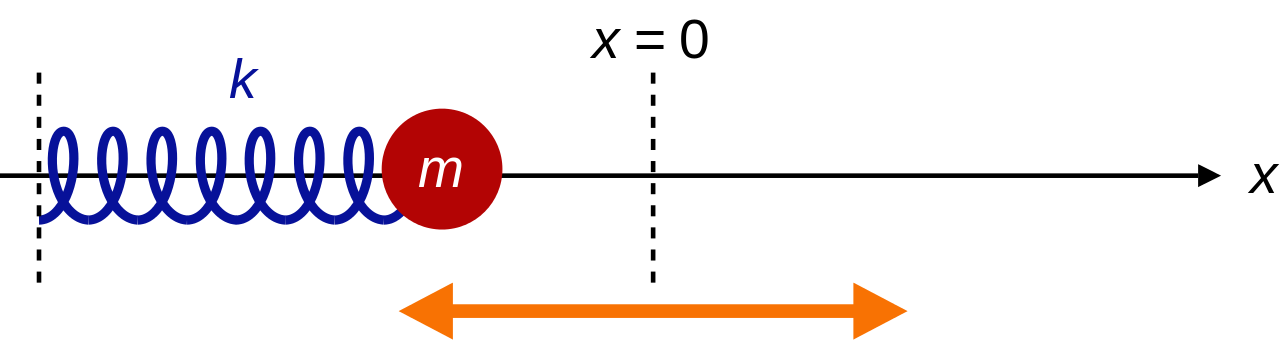
\includegraphics[width=0.6\textwidth]{figures/SHO_lagrangian_mech.png}
    %}{An oscillating spring}
    \caption{A spring with a mass on the end oscillating around equilibrium at $x=0$.}
\end{figure}

\paragraph{Example 5.1:} Consider the work done to stretch a spring. The greater the force, the more the spring stretches. The force needed to stretch the spring is proportional to its extension, $F= kx$, this is a version\footnote{For completeness note that here the force is a force acting on the spring to extend it, thus the force is pointing in the positive direction, when we return to Hooke's law in later weeks we will be discussing the springs natural restoring force which always points towards equilibrium, in that case the sign in Hooke's law will be negative.} of what is called \textbf{Hooke's Law}. We will return to Hooke's law in detail later in the module. The constant of proportionality $k$ that appears in Hooke's law is called the \textbf{spring constant} and it is a measure of how stiff, or difficult to stretch a spring is. If we plotted force against extension for Hooke's law we get a straight line, and the area under the line is the area of a triangle of base $x$ and height $F$. Thus
\begin{equation*}
W_{\text{spring}}=\frac{1}{2}F x=\frac{1}{2}k x^{2}.
\end{equation*}

\begin{figure}[ht]
    \centering
    \ThisAltText{ A plot of force against extension for a spring showing that there is a linear relationship.}
    %\pdftooltip{
    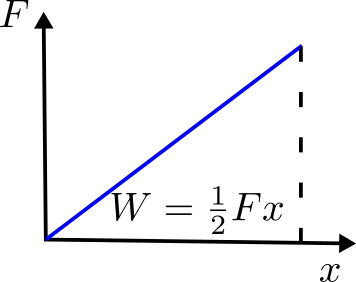
\includegraphics[width=0.4\textwidth]{figures/spring_work.png}
    %}{force against extension for a spring}
    \caption{A plot of applied force against extension for a spring.}
    \label{fig: spring extension}
\end{figure}


\paragraph{Kinetic Energy:} Kinetic energy is the energy of an object due to its motion. The faster an object moves the more kinetic energy it has. Kinetic energy is denoted by $K$ or $E_{K}$ and is also measured in Joules. We will make a lot of use of it when understanding how objects are moving. Note that for our purposes we can think of energy as a book keeping tool in the same way as momentum, though it plays quite a fundamental roll in understanding many areas of physics.\\

We can derive an equation for kinetic energy by making use Newton's second law, the formula for work, and one of the kinematic equations. Consider an object of mass $m$ starting at rest and acted on by a force $F$, resulting in it having a velocity $v$ after a time $t$. While accelerating the object has travelled
\begin{equation*}
s=\frac{1}{2}\left(u+v\right)t=\frac{1}{2}vt,
\end{equation*}
and has an acceleration of $a=\frac{v}{t}$. From Newton's second law we know that the force is given by
\begin{equation*}
F=ma=\frac{mv}{t}.
\end{equation*}
Thus the work done is
\begin{equation*}
W=Fs=\frac{1}{2}mv^{2}.
\end{equation*}
The object has gained energy from the work being done on it.

This expression holds true more generally and we call 
\begin{equation}
E_{K}=\frac{1}{2}mv^{2}
\label{eq: kinetic energy}
\end{equation}
the kinetic energy.

%
\paragraph{Potential Energy:}  Another type of energy that is relevant to the study of moving objects is the \textbf{potential energy}. This is the energy that an object has due to its position. Think of an object at rest at the top of a hill. It has no kinetic energy, but a lot of potential energy as it could gain potential energy by rolling down the hill. Sometime we would say that the object has the potential to do work.\\

If an object of mass $m$ is raised a vertical height $\Delta h$ as a steady speed, the force needed to raise the object is equal and opposite to its weight $W=mg$. Think of picking up an apple or a bag of sugar, you have to exert a force that balances teh weight of teh object to pick it up. The work done is then
\begin{equation*}
W=Fs=mg\Delta h.
\end{equation*}
The object now has the potential to do work if it falls so the (gravitational) potential energy is 
\begin{equation}
E_{P}=mg\Delta h.
\label{eq: potential energy}
\end{equation}

Note that some places will use $K$ for   kinetic energy and $U$ or $V$ for potential energy. In this module we will try to stick with $E_{K}$ and $E_{P}$ but be warned that not every book uses this notation.\\

\textbf{Warning:} Energy is a scalar quantity and as such is always positive\footnote{At least in most conventions, though you may find some older books that do not follow this approach.}, you may object to this saying that in $E_{P}$ we have $g$ and that is negative. However, when working with potential energy we are really working with $\vert g\vert =9.8\text{m/s}^{2}$. The formula is almost never quoted with the modulus signs and it is usually left to the reader to understand what is going on. Here, we will try to make clear the situations when we are really talking about $g$ and when we are talking about $\vert g\vert$.\\

Energy can change form between kinetic and potential, and other forms of energy that you may meet later on.  This was already suggested when we discussed how an object with potential energy at the top of a hill can lose potential energy, but gain kinetic energy by rolling down the hill. Consider an object of mass $m$ that has been raised to a height $h$, such that it has potential energy $E_{P}=mgh$. If the object is released it will accelerate as it falls, and the potential energy will become kinetic energy. After falling a distance $s$ it has kinetic energy equal to the change in kinetic energy
\begin{equation*}
\frac{1}{2}mv^{2}=mg h.
\end{equation*}
Note that since $g$ is only approximately constant \textbf{near} the surface of the Earth, if an object falls a great distance, or from a very great height, we will need to take account of the change in $g$.\\

Note that the conversion between kinetic and potential energy will not always be perfect, if there is air resistance, or friction of some kind then energy can be lost to heat or sound, and the gain in kinetic energy will be less than the loss of potential energy. We think of this loss as being due to an average frictional force acting over the whole of the objects motion. This force is found by associating the difference between the potential and kinetic energy with a work done by the object on the air or on the track that it is moving along. Then the average frictional force is given by
\begin{equation*}
F=\frac{W}{s}=\frac{E_{P}-E_{K}}{s}.
\end{equation*}

\paragraph{Example 5.2:} Consider a fairground ride whose track descends a vertical drop of $55\text{m}$ over a section of rails of length $120\text{m}$. A train of mass $2500\text{kg}$ on the track reaches a speed of $30\text{m/s}$ at the bottom of the descent after being at rest at the top. Find:
\begin{itemize}
\setlength{\itemsep}{-5pt}
    \item[a)] The potential energy lost by the train after descending.
    \item[b)] The gain in potential energy after the train has reached the bottom.
    \item[c)] The average frictional force on the train during the descent.
\end{itemize} 
a) The loss in potential energy is given by
\begin{equation*}
E_{P}=mg\Delta h=2500\times 9.8\times 55=1.35\times 10^{6}\text{J}.
\end{equation*}

b) The kinetic energy starts as $0\text{J}$ since the train is at rest, at the bottom it is
\begin{equation*}
E_{K}=\frac{1}{2}mv^{2}=\frac{1}{2}\times 2500\times (30)^{2}=1.13\times 10^{6}\text{J}.
\end{equation*}

c) The work done by the train on the rails and on the air is the difference between $E_{K}$ and $E_{P}$, $W=E_{P}-E_{K}=2.2\times 10^{5}\text{J}$, so the average frictional force is
\begin{equation*}
F=\frac{W}{s}=\frac{2.2\times 10^{5}}{120}=1830\text{N}.
\end{equation*}

\section{Power and Efficiency}
Energy can be transferred from one object to another in several ways. We have already seen that when an object rolls down a hill or falls down that the gravitational potential energy is transferred into kinetic energy. Energy is also transferred when an object does work, for example it causes a force to act on another object and transfers its energy to the other object, we will meet examples of this later when we discuss what happens to energy during a collision.\\

In the example that we saw earlier of potential energy swapping to kinetic energy imperfectly we said that the object lost energy to friction with the track and air resistance. This energy has not disappeared but has become heat energy or sound energy.  Since heat is a kind of energy\footnote{The study of heat is known a \textbf{thermodynamics} and is a major area of physics. Those of you on engineering and physics degrees will learn more about thermodynamics in future modules.}, the transfer of heat between objects is another kind of energy transfer. Heat can be transferred in essentially three ways: \textbf{Conduction}, \textbf{Convection}, \textbf{Radiation}. In addition, electricity, sound waves, and electromagnetic radiation\footnote{like light} will all transfer energy.\\

\textbf{Power} is the rate of transfer of energy, or the rate of change of energy. The unit of power is the Watt, with $1\text{W}=1 \text{J}/\text{s}$. The units is named after James Watt a Scottish inventor and engineer who was an early pioneer of steam engines. Mathematically the relationship between power, $P$, energy, $E$, and time, is given by
\begin{equation}
P=\frac{\Delta E}{\Delta t}.
\label{eq: PET equation}
\end{equation}
As was the case with the other rates of change we have met, this formula just gives the average power. The instantaneous power is given by the derivative of the energy. The formula is often given without the deltas as shown in the frmula triangle in \cref{fig: PEt triangle}. If a force does work then the power is the work done per second or 
\begin{equation*}
P=\frac{\Delta W}{\Delta t}.
\end{equation*}

\begin{figure}[ht]
    \centering
    \ThisAltText{ The formula triangle for energy, power, and time.}
    %\pdftooltip{
    \large \formulatriang[.4]{$E$}{}{$ P$}{}{$ t$}{}
    %}{The formula triangle for power, change in energy, and change in time.}
    \caption{The formula triangle for power, change in energy, and change in time. }
    \label{fig: PEt triangle}
\end{figure}

\paragraph{Example 5.3:} Consider a person of weight $690\text{N}$ who climbs a slight of stairs with height $10\text{m}$ in $12\text{s}$.  What is the power of their leg muscles?\\

The work done is:
\begin{align*}
W	&=Fs\\
	&=690\times 10=6900 \text{J}.
\end{align*}
The power due to this work done is then
\begin{align*}
P&=\frac{W}{t}\\
	&=\frac{6900}{12}\\
	&=575\text{W}.
\end{align*}
Thus each leg has a muscle power of $287.5\text{W}$.\\

For an engine the output power is sometimes called the \textbf{motive power}, as it is power available to cause motion, such as a steam engine on a train where the output power of the engine is used to move the train. For a powered vehicle driven by a constant force $F$ to move at a speed $v$, the power is given by
\begin{equation*}
P=Fv.
\end{equation*}
Can you see how to derive this from \cref{eq: PET equation} given the relationship between work done and force?

\paragraph{Example 5.4:} Consider an aircraft powered by engines which exert a force of $40\text{kN}$. The aircraft is in level flight at a constant velocity of $80\text{m/s}$. Calculate the power output of the engines at this speed.\\

First note that since we know a force and a velocity we will want to use $P=Fv$ to compute the power. We are given that $F=40\text{kN}=40000\text{N}$, and $v=80\text{m/s}$, thus
\begin{equation*}
P=Fv=40000\times 80 = 3.2\times 10^{6}\text{W}.
\end{equation*}


\paragraph{Example 5.5:} A person of weight $450\text{N}$ climbed $2.5\text{m}$ up a rope in $18\text{s}$. Calculate:
\begin{itemize}
\setlength{\itemsep}{-5pt}
    \item[a)] The gain in potential energy.
    \item[b)] The useful energy transfer per second, this is another name for the power.
\end{itemize} 

a) Use $E_{P}=mg\Delta h$ with $mg =450\text{N}$ and $\Delta h= 2.5$ so that
\begin{equation*}
E_{P}=mg\Delta h=450\times 2.5 =1125\text{J}\simeq 1.1\text{kJ}.
\end{equation*}

b) The useful energy transfer is the power and $P=W/t$ so 
\begin{equation*}
P=\frac{E_{P}}{t}=\frac{1125}{18}=62.5\text{W}.
\end{equation*}

\paragraph{Example 5.6:} An electric motor operating a sliding door exerts a force of $125\text{N}$ on the door causing it to open at a constant speed of $0.4 \text{m/s}$. What is the output power of the motor?\\

The output power is given by
\begin{equation*}
P=Fv=125\times 0.4 =50\text{W}.
\end{equation*}
The motor must transfer $50\text{J}$ of energy to the door every second while it is being opened.\\

Does all the energy supplied to the motor get used to open the doors? No, friction in the motor's bearings and electrical resistance in the wires mean that some of the electrical energy supplied to the motor is wasted. There will also be energy wasted if the motor makes a noise while it is working. For example, if the motor gets electrical energy at a rate of $150\text{J/s}$ and transfers $50\text{J/s}$ to the door then $100\text{J/s}$ is wasted due to friction, resistance, and sound. The fact that not all of the energy used is useful brings us on to the concept of \textbf{efficiency}.\\

The efficiency is the ratio of the useful energy to the total energy. It is often given the symbol $\epsilon$ and is given by the formula
\begin{equation*}
\epsilon =\frac{\text{Useful energy}}{\text{Total energy supplied}}.
\end{equation*}

\paragraph{Example 5.7:}  A $500\text{W}$ electric winch raises a $150\text{N}$ weight by $6\text{m}$ in $10\text{s}$. How much energy is wasted and what is the efficiency of the winch?\\

The electrical energy supplied to the winch while it is opperating is
\begin{equation*}
E=Pt=500\times 10=5000\text{J} = 5\text{kJ}.
\end{equation*}
However, the useful energy is the energy required to lift the weight, i.e. the potential energy gain of the weight which is
\begin{equation*}
\Delta E_{P}=mg \Delta h=150\times 6=900\text{J}=0.9\text{kJ}.
\end{equation*}
The diffrence between these two is the wasted energy
\begin{equation*}
\Delta E= E-\Delta E_{P}=5-0.9=4.1\text{kJ},
\end{equation*}
the efficiency is thus 
\begin{equation*}
\epsilon =\frac{0.9}{5}=0.18.
\end{equation*}

As well as expressing the efficiency using $\epsilon$, sometimes you will come across the percentage efficiency. This is just $\epsilon\times 100\%$. So in the last example the efficiency is $18\%$. We can also talk about efficiency whenever we have a change of energy, for example when we discussed the frictional force acting on moving objects we could also have phrased that as an efficiency. \\

A problem that people often study, particularly in material science of branches of engineering, is how to boost the efficiency when transferring energy. This is often rephrased as saying ``Is it possible to stop energy being lost as heat or sound?''\\

Consider a petrol or diesel engine in a car. This loses a lot of energy to heat as well as to sound. We could stop the engine loosing heat to the environment by insulating it, but then the engine would heat up itself until it stops working.  A similar example is a filament light bulb. These work by passing a current through a piece of wire, the filament, with a high resistance so that the wire will heat up and glow, creating light. In a sense the light is just a by product of the filament heating up. For example a filament bulb is around $12\%$ efficient with most of the energy wasted as heat, a fluorescent lamp is around $80\%$ efficient, and LED lights can be even better.\\

We can also think about the different sources of energy that we use to power our homes, in particular the renewable sources of energy like wind, solar, and hydro. In \textbf{STM0002 Group Project} the computer science and engineering students will see more about this and one of the project options is to explore different types of renewable energy generation. The important point here is that different types of energy generation will have different efficiencies, for example a wind turbine can be at most $60\%$ efficient, this is known as Betz's law and it can be fun to think about why there is this theoretical efficiency limit and what it means.\\

Since power is energy per second we can also think of the efficiency as the ratio of the usable power to the total power produced. This is particularly useful when thinking about power stations as the usable power will be the electrical power generated, while the total power is the energy supplied per second by the fuel, e.g. by burning coal or gas, or from the wind.

\paragraph{Example 5.8:} Consider a power station with an overall efficiency of $35\%$ which produces $200\text{MW}$ of electrical power. The fuel used in the power station releases $80\text{MJ}$ per kilogram of fuel burned. Calculate:
\begin{itemize}
\setlength{\itemsep}{-5pt}
    \item[a)] The energy per second supplied by the fuel,
    \item[b)] The mass of fuel that is burned per day.
\end{itemize} 

a) The energy per second supplied by the fuel is the total power, recall that $P=E/t$. We know that the power station is $35\%$ efficient so
\begin{equation*}
0.35=\frac{200\text{MW}}{\text{energy supplied per second}}
\end{equation*}
so
\begin{equation*}
\text{energy supplied per second}=\frac{200000}{0.35}=570\frac{\text{MJ}}{\text{s}}.
\end{equation*}

b) We get $80\text{MJ}$ for every kilogram of fuel burned so we need to burn $570/80=7.125\text{kg}$ every second to supply the claimed power. Thus we need to burn 
\begin{equation*}
7.125\times 60\times 60\times 24=6.2\times10^{5}\text{kg}
\end{equation*}
of fuel every day.


\section{Energy and Collisions}
In the last section we analysed collisions using conservation of momentum, at the end we said that there are two types of collision:
\begin{itemize}
\setlength{\itemsep}{-5pt}
    \item Elastic collisions where both momentum and kinetic energy are conserved.
    \item Inelastic collisions where momentum is conserved but the kinetic energy is not.
\end{itemize} 
Sometimes a distinction is made between inelastic collisions where the kinetic energy decreases, just called inelastic, and where the kinetic energy increases, called \textbf{explosions}. \\

In an inelastic collision either some of the kinetic energy is transferred into another kind of energy such as heat, or a different kind of energy, such as chemical energy, is transferred into kinetic energy. If we looked at the total energy rather than just the kinetic energy we would see that the total energy is conserved.\\

\paragraph{Example 5.9:} A ball of mass $m$ falls from a height $H$ and rebounds off the floor to a height $h$. How does the kinetic energy change during the motion?\\

The kinetic energy before the impact is the loss of potential energy when the ball falls from its original height, $E_{P}=mgH$. While the kinetic energy after the impact will be equal to the potential energy that the ball has when it reaches the new height $h$, $E_{P}=mgh$. If the kinetic energy is conserved (ie the collision is elastic) then $h=H$ and the ball returns to the height it started at. However, if the collision with the floor produces sound or the floor heats up the the final height will be less than the initial height, $h<H$ and the collision was inelastic.

\paragraph{Example 5.10:} Consider a railway wagon of mass $8000\text{kg}$ moving at $3.0\text{m/s}$ before colliding with an initially stationary wagon of mass $5000\text{kg}$. The two wagons separate after the collision, and the $8000\text{kg}$ wagon moves at a speed of $1\text{m/s}$ without changing its direction. Calculate:
\begin{itemize}
\setlength{\itemsep}{-5pt}
    \item[a)] The speed and direction of the $5000\text{kg}$ wagon after the collision,
    \item[b)] The change in kinetic energy of the wagons due to the collision.
\end{itemize} 

a) The initial momentum is 
\begin{equation*}
p_{i}=8000\times 3 +5000\times 0=24 000\frac{\text{kg m}}{\text{s}}.
\end{equation*}
Let us call the final velocity of the $5000\text{kg}$ wagon $v_{B}$, then the final momentum is
\begin{equation*}
p_{f}=8000\times 1 +5000\times v_{B}=8000+5000v_{B}.
\end{equation*}
Conservation of momentum implies that $p_{i}=p_{f}$ or that
\begin{align*}
24 000&=8000+5000v_{B},\\
\Rightarrow v_{B}&=\frac{24000-8000}{5000}\\
&=\frac{16000}{5000}=3.2\text{m/s}.
\end{align*}
So the $5000\text{kg}$ wagon is moving in the same direction as the $8000\text{kg}$ wagon but at a speed of $3.2\text{m/s}$.\\

b) Now we repeat the same analysis but calculate the kinetic energies rather than the momentum. The inital kinetic energy is
\begin{equation*}
E_{K_{i}}=\frac{1}{2}\times 8000\times(3)^2 +\frac{1}{2}\times 5000\times 0=36000\text{J}.
\end{equation*}

After the collision the kinetic energy is
\begin{equation*}
E_{K_{f}}=\frac{1}{2}\times 8000\times 1^{2}+\frac{1}{2}\times 5000\times (3.2)^{2}=29 600\text{J}.
\end{equation*}

The change in kinetic energy is then
\begin{equation*}
E_{K_{i}}-E_{K_{f}}=36000-29600=6400\text{J}.
\end{equation*}
Thus the total kinetic energy of the system has decreased by $6400\text{J}$.\\


Several of the problems on the tutorial sheet will get you to revisit collisions that you have previously studied using momentum so that you can see what happens to the mechanical energy in these cases.


%%%%%%%%%%%%%%%%%%%%%%%%%%%%%%%%%%%%%%%%%%%%%%%%%%%%%%%%%%%%%%%%%%%%%%%

\chapter{Motion in a Circle}
\section{Radians and Degrees}
To discuss circular motion we need to know how to describe angles, eg how round in a circle we have gone. Often when working with circles we do not describe angles in terms of degrees but instead use units called radians.  You are likely to be familiar with describing angles in a degrees where a full rotation is $360^{\circ}$ and a half rotation is $180^{\circ}$. \textbf{Radians} are an alternative, and some would say ``better'' method of measuring angles, the certainly simplify some computations, though they can seem confusing when we first meet them.\\

The basic idea of radians is to work in terms of the distance around the circle that the angle corresponds to.  For a circle with radius $r$ the circumference is $c=2\uppi r$, while an arc of the circle would have length s, shown in red in \cref{fig: radians}. Radians are defined in terms of the length of arcs as
\begin{equation}
\uptheta =\frac{s}{r},
\label{eq: definition of radians}
\end{equation}
in other words, an angle measured in radians is the ratio of the distance travelled on an arc round the circle to the radius of the circle. 
This means that a full rotation $360^{\circ}$ corresponds to $2\uppi$ radians as in this case $s=2\uppi r$, half a rotation or $180^{\circ}$ then corresponds to $\uppi$ radians. 

\begin{figure}[ht]
    \centering
    \ThisAltText{ A circle of radius r demonstrating the relationship between arc length and angle.}
    %\pdftooltip{
    \begin{tikzpicture}
   % \draw[step=1cm,gray,very thin] (3,-3) grid (3,3);
   \filldraw[color = blue, ultra thick](0,0) circle (0.05);
    \draw[ ultra thick](0,0) circle (2);
    \draw[ultra thick] (0,0) -- (1.414,1.414);
  \node[anchor =south] at (0.7,0.7) {$r$};
    \draw[ultra thick] (0,0) -- (2,0);
    \draw[ultra thick] (1,0) arc (0:45:1) node[anchor=north]{$\uptheta$};
     \draw[ultra thick, color=red] (2,0) arc (0:45:2) node[anchor=north]{$s$};
    \end{tikzpicture}
    %}{A circle}
    \caption{A circle of radius $r$ showing how arc length around the circle corresponds to angles}
        \label{fig: radians}
\end{figure}

More generally the conversion rule is that
\begin{equation*}
\text{radians} = \frac{180^{\circ}}{\uppi}\times \text{degrees}.
\end{equation*}
The main advantage of radians comes when differentiating and expanding functions as working in degrees requires extra terms to be included and greater care to be taken. While we will not be doing any differentiation in this module we will come across some expressions where we need to work in radians for the quoted expressions to be valid. When this happens we will include a warning so that it is clear where you need to be careful.\\

One way to motivate working in radians is to think of unwinding the circle to get a straight line, for a circle of radius $r$ this length will be the circumference, if we divide this length by $r$ we will have a line if length $2\uppi$ and the angle in radians will be the distance travelled along this line. In other words, working in radians is a bit like converting from circular motion to linear motion.

\begin{figure}[ht]
    \centering
    \ThisAltText{ Another circle showing how the arc length and angle can be related to a straight line distance.}
   % \pdftooltip{
    \begin{tikzpicture}
   % \draw[step=1cm,gray,very thin] (3,-3) grid (3,3);
   \filldraw[color = blue, ultra thick](0,0) circle (0.05);
    \draw[ ultra thick](0,0) circle (2);
    \draw[ultra thick] (0,0) -- (1.414,1.414);
 % \node[anchor =south] at (0.7,0.7) {$r$};
    \draw[ultra thick] (0,0) -- (2,0);
    \draw[ultra thick] (1,0) arc (0:45:1) node[anchor=north]{$\uptheta$};
     \draw[ultra thick, color=red] (2,0) arc (0:45:2) node[anchor=north]{$s$};
     \draw[ultra thick] (6,-3.14) --(6,3.14);
     \draw[ultra thick, color = red] (6,-3.14) --(6,-2.355) node[anchor=west]{$\uptheta$};
     \draw[ultra thick, ->] (2.5,0) -- (5.5,0);
    \end{tikzpicture}
   % }{A circle}
    \caption{A circle of radius $r$ showing how arc length around the circle corresponds to angles}
        \label{fig: radians 2}
\end{figure}

As evidenced in \cref{fig: radians,fig: radians 2}, it is common practice to use the Greek letter theta, $\uptheta$, to denote an angle. Other Greek letters like phi, $\upphi$ or $\upvarphi$, and psi, $\uppsi$, are sometimes used as well. It is worth spending some time familiarising yourself with these Greek letters so you do not think that they are just badly written English letters.

\section{Circular Motion}
In the second section of these notes we studied linear motion, in particular uniform motion where the acceleration is constant. In that case objects moved in straight lines. What about if an object is moving in a circle?\\

An object rotating at a steady rate is said to be in \textbf{uniform circular motion}. A good example to have in mind is a point on the perimeter of a wheel of radius $r$ rotating at a steady speed. The circumference of the wheel is $2\uppi r$ and we call the time taken for $p$ to rotate once around the wheel the \textbf{period} $T$. Another important quantity related to the period is the \textbf{frequency}, $f=1/T$ which measures the number of rotations per second. The period is measured in seconds as it is a unit of time, while the frequency is measured in Hertz or units of per second.\\

\begin{figure}[ht]
    \centering
  %  \pdftooltip{
  \ThisAltText{ A rotating wheel with a point and its instantaneous straight line velocity marked.}
    \begin{tikzpicture}
   % \draw[step=1cm,gray,very thin] (3,-3) grid (3,3);
   \filldraw[color = blue, ultra thick](0,0) circle (0.05);
    \draw[ ultra thick](0,0) circle (2);
    \draw[ultra thick, color=blue] (0,0) -- (1.414,1.414);
    \draw[ultra thick] (0,0) -- (2,0);
     \filldraw[color = blue, ultra thick](1.414,1.414) circle (0.05)node[anchor=west]{$p$};
     \draw[ultra thick, color=red, ->] (1.414,1.414)-- (0.5,2.33)node[anchor=west]{$v$};
    \end{tikzpicture}
  %  }{A rotating wheel}
    \caption{A rotating wheel with a point $p$ marked on its surface along with the instantaneous velocity of $p$.}
        \label{fig: pt on a wheel}
\end{figure}

The linear speed, or the speed if the point $p$ was moving in a straight line is 
\begin{equation*}
v=\frac{\text{circumference}}{T}=\frac{2\uppi r}{T}=2\uppi r f.
\end{equation*}
This relationship gives us away to convert between the linear motion of an object and the circular motion of its wheels.


\paragraph{Example 6.1:} A cyclist is travelling at $25\text{m/s}$ on a bicycle that has wheels of radius $750 \text{mm}$. Calculate:
\begin{itemize}
\setlength{\itemsep}{-5pt}
    \item[a)] The time for one rotation of the wheel,
    \item[b)] The rotation frequency of the wheel,
    \item[c)] The number of times the wheel rotates in a minute.
\end{itemize} 

a) Rearranging $v=2\uppi r/T$ and substituting in the numbers we have that the period is
\begin{equation*}
T=\frac{2\uppi r}{v}=2\uppi\times \frac{0.75}{25}=0.19\text{s}.
\end{equation*} 

b) The frequency is 
\begin{equation*}
f=\frac{1}{T}=\frac{1}{0.19}\text{Hz}=5.3\text{Hz}.
\end{equation*}

c) The number of rotations in a minute is then
\begin{equation*}
\text{rotations per minute} = f\times 60=320.
\end{equation*}

The angle $\uptheta$ that a rotating object moves through is called the \textbf{angular displacement}. We will almost always work with $\uptheta$ in radians, though occasionally you may see an angle quoted in degrees that you need to convert into radians. In uniform circular motion an object turns through an angle of $2\uppi/T$ radians per second, thus the angular displacement after a time $t$ is
\begin{equation}
\uptheta=\frac{2\uppi t}{T}.
\end{equation}
To understand this recall that the total distance round the circle is $2\uppi$ in radians, and $T$ is measuring the time it takes to complete a full rotation. The angular displacement is measured in radians as it is an angle. \\

The angular analogue of the speed from linear motion is the \textbf{angular speed} or angular velocity, omega  $\upomega$, which is defined as the rate of change of angular displacement and is given by
\begin{equation}
\upomega=\frac{\uptheta}{t}=\frac{2\uppi}{T}=2\uppi f.
\end{equation}
we measure angular speed in units of radians per second or $\text{rad/s}$. 

\paragraph{Example 6.2:} Consider a cyclist travelling at $ 12\text{m/s}$ on a bike with wheels of radius $0.4\text{m}$. Calculate:
\begin{itemize}
\setlength{\itemsep}{-5pt}
    \item[a)] The frequency of rotation of the wheels,
    \item[b)] The angular speed of each wheel,
    \item[c)] The angle that a wheel turns through in $0.1\text{s}$ in both radians and degrees.
\end{itemize} 

a) The circumference of a wheel is $2\uppi r=2\uppi\times 0.4 =2.5\text{m}$ and 
\begin{equation*}
T=\frac{\text{circumference}}{v}=\frac{2.5}{12}=0.21\text{s}.
\end{equation*}
The frequency is thus
\begin{equation*}
f=\frac{1}{T}=\frac{1}{0.21}=4.8\text{Hz}.
\end{equation*}

b) The angular speed is 
\begin{equation*}
\upomega=2\uppi f=30\text{rad/s}.
\end{equation*}

c) The angular displacement in $0.1\text{s}$ is
\begin{equation*}
\uptheta=\upomega t=3 \text{rad},
\end{equation*}
or in degrees this is $3\times360^{\circ}/2\uppi=170^{\circ}$.

\section{Centripetal forces}
When an object is moving in a circle at a constant speed the linear velocity is constantly changing direction. In other words the magnitude of the velocity is constant but its direction is changing. Since the objects velocity is changing in time it is accelerating. This may seem counter intuitive since we say that the motion is uniform. \\

From \cref{fig: pt on a wheel}  we see that the velocity is tangent to the circle at the objects location. As the object moves around the circle the direction of the velocity continually changes with the direction of change being towards the centre of the circle. Thus the acceleration is pointing towards the centre of the circle. This acceleration is called the \textbf{centripetal acceleration}, and is given by
\begin{equation}
a=\frac{v^{2}}{r}=\upomega^{2}r.
\label{eq: centripetal acceleration}
\end{equation}


\begin{figure}[ht]
    \centering
    \ThisAltText{ A rotating wheel with a point, its instantaneous velocity, and its centripetal acceleration marked.}
    %\pdftooltip{
    \begin{tikzpicture}
   % \draw[step=1cm,gray,very thin] (3,-3) grid (3,3);
   \filldraw[color = blue, ultra thick](0,0) circle (0.05);
    \draw[ ultra thick](0,0) circle (2);
    \draw[ultra thick, color=blue,->] (1.414,1.414)node[anchor=north]{$a$}--(0.5,0.5);
 % \node[anchor =south] at (0.7,0.7) {$r$};
    \draw[ultra thick] (0,0) -- (2,0);
  %  \draw[ultra thick] (1,0) arc (0:45:1) node[anchor=north]{$\ut$};
     %\draw[ultra thick, color=red] (2,0) arc (0:45:2) node[anchor=north]{$s$};
     \filldraw[color = blue, ultra thick](1.414,1.414) circle (0.05)node[anchor=west]{$p$};
     \draw[ultra thick, color=red, ->] (1.414,1.414)-- (0.5,2.33)node[anchor=west]{$v$};
    \end{tikzpicture}
   % }{A rotating wheel with v and a marked}
    \caption{A rotating wheel with a point $p$ marked along with its velocity and acceleration.}
        \label{fig: pt on a wheel 2}
\end{figure}


To make an object move in a circular path we need to act on it with a force that generates the inward acceleration. This resultant force is known as the \textbf{centripetal acceleration} and it acts towards the centre of the circle.\\

There are a few places where you may have come across centripetal acceleration before:
\begin{itemize}
\setlength{\itemsep}{-5pt}
    \item Satellites orbiting the earth get their centripetal force from the Earth's gravity.
    \item An object spinning round on the end of a string gets its centripetal force from the string's tension.
\end{itemize} 

For an object moving with linear velocity $v$ along a circular path of radius $r$ we know the centripetal acceleration from \cref{eq: centripetal acceleration}. By Newton's second law this corresponds to a centripetal force given by
\begin{equation}
F=m\upomega^{2}r=\frac{mv^{2}}{r}.
\label{eq: centripetal force}
\end{equation}

Note that since the centripetal force is at right angles to the direction of motion it does no work, and the kinetic energy is constant since the speed is unchanged.

%\paragraph{Example 6.3:} The wheel of the London Eye has a diameter of $130\text{m}$ and takes $30\text{min}$ for one full rotation. Calculate:
\begin{itemize}
\setlength{\itemsep}{-5pt}
    \item[a)] The speed of a capsule,
    \item[b)] The centripetal acceleration of a capsule,
    \item[c)] The centripetal force acting on a person of mass $65\text{kg}$ in a capsule.
\end{itemize} 

%a) The circumference is 
\begin{equation*}
2\uppi r=\uppi d=\uppi \times 130=408\text{m},
\end{equation*}
and the speed is 
\begin{equation*}
v=\frac{2\uppi r}{T}=\frac{408}{30\times 60}=0.23\text{m/s}.
\end{equation*}

b) The centripetal acceleration is 
\begin{equation*}
a=\frac{v^{2}}{r}=\frac{0.23^{2}}{65}=0.00079\text{m/s}^{2}=7.9\times 10^{-4}\text{m/s}^{2}.
\end{equation*}

c) The centripetal force is then 
\begin{equation*}
F=ma=65\times 7.9\times 10^{-4}=5.1\times 10^{-2}\text{N}.
\end{equation*}

%Notice that the centripetal force points inwards. Sometimes when people talk about circular motion they will mention an outward pointing centrifugal force. This is a \textbf{fictitious force} which appears if you work in the \textbf{reference frame} of the rotating object. The Coriolis force is another fictitious force that appears due to the rotation of an object. It is important to note here that fictitious does not mean that we are imagining these effects, but rather that they are not due to forces. They occur because we are in a rotating reference frame. If you go on to study more physics then you will learn more about why rotational motion results in these fictitious forces.

\section{Circular motion in action}
To finish off this section we will now discuss some concrete examples of where objects moving in circles appear in the real world:
\begin{itemize}
\setlength{\itemsep}{-5pt}
    \item Vehicles going round roundabouts.
    \item Going over hills.
    \item Banked tracks.
    \item Amusement rides
\end{itemize} 
All four of these examples are included in \citep{breithaupt2016aqa} so you can look there for further details if you want to know more.  For the case of motion on a banked track we refer the interested reader to Chapter 17.3 of \citep{breithaupt2016aqa}.

\paragraph{Going over hills.} Consider a vehicle of mass $m$ moving at speed $v$ along a road that passes over the top of a hill or a curved bridge. We will assume that the road or bridge has the shape of an arc in a circle, this may not be perfectly true but it is a good approximation and in this module we will not need to take a better approximation. The road acts on the vehicle through a support force $S$ which is opposite to the vehicle's weight $mg$. The difference between the support force and the weight acts towards the centre of the circle. This net force is a centripetal force and is given by
\begin{equation*}
mg-S=\frac{mv^{2}}{r}.
\end{equation*}
Here $r$ is the radius of curvature of the hill, in other words the radius of the circle if we pretend that the hill is part of a circle.\\

\textcolor{red}{Figures to be added to this section.}\\

If the vehicle is travelling fast enough it will lose contact with the road. This will happen for velocities higher than a critical speed $v_{0}$. When $v=v_{0}$ the support force will vanish and
\begin{equation*}
mg=\frac{mv^{2}_{0}}{r}.
\end{equation*}
As there is a factor of the mass on both sides of the equation they cancel out and we are left with the critical speed given in terms of $g$ and the radius of the circle as
\begin{equation*}
v_{0}=\pm\sqrt{gr},
\end{equation*}
the $\pm$ show that the vehicle can be heading either left or right over the hill and the condition is the same. As $g$ is approximately constant on Earth, this is essentially a geometric condition where the size of the hill determines how fast you need to go to lose contact with the road. For small hills this may not be that fast, but for a large hill you would need to go very fast.\\

If $r=5\text{m}$ then $v_{0}=\pm 7\text{m/s}$ or $15.7\text{mph}$.

\paragraph{Roundabouts.} Next consider a car of mass $m$ going in a circle round a roundabout at a speed $v$. Now the car is going round in a horizontal circle rather than a vertical circle. The centripetal force is not related to the weight of the car but rather to the sideways frictional force between the car's tires and the road,
\begin{equation*}
F_{f}=\frac{mv^{2}}{r}.
\end{equation*}
The weight of the vehicle is still important though. If the vehicle is travelling too fast, above a critical velocity $v_{0}$, then the friction will not be enough to stop the car from slipping and skidding. The limiting force is given by
\begin{equation*}
F_{0}=\frac{mv_{0}^{2}}{r}.
\end{equation*}
As $F_{0}$ is a frictional force it can be written as $F_{0}=\upmu mg$ where $\upmu$ is the \textbf{coefficient of friction}\footnote{There are actually two types of coefficients of friction: static and dynamic. In this module we do not make a distinction between them, but it is important to be aware that there is a difference as some books will use different names in different contexts.}.  Using $\upmu$ we can find an expression for $v_{0}$ analogous to that used above. The critical speed is given by
\begin{equation*}
v_{0}=\sqrt{\upmu g r},
\end{equation*}
deriving this expression is left as an exercise to the interested reader.

\paragraph{Example 6.4:} Consider a vehicle of mass $1200\text{kg}$ passing over a circular bridge whose radius of curvature is $15\text{m}$ at a speed of $10\text{m/s}$. Calculate:
\begin{itemize}
\setlength{\itemsep}{-5pt}
    \item[a)] The centripetal acceleration of the vehicle on the bridge,
    \item[b)] The support force on the vehicle when it is at the top of the bridge,
    \item[c)] The critical velocity at which the vehicle will lose contact with the road.
\end{itemize} 


a) The centripetal acceleration is found by solving 
\begin{equation*}
ma=F_{c}=\frac{mv^{2}}{r},
\end{equation*}
for $a$. In other words
\begin{equation*}
a=\frac{v^{2}}{r}=\frac{10^{2}}{15}=6.67\text{m/s}^{2}.
\end{equation*}

b) The support force is given by the difference between the cars weight and the centripetal force,
\begin{equation*}
S=mg-\frac{mv^{2}}{r}=mg-ma=m\left(g-a\right)=1200\left(9.8-6.67\right)=3756\text{N}\sim 3.8\text{kN}.
\end{equation*}

c) At the critical velocity we have that $S=0$ and $v_{0}=\sqrt{gr}$ so can just substitute the given value of $r$ into this expression to find
\begin{equation*}
v_{0}=\sqrt{gr}=\sqrt{9.8\times 15}=12.1\text{m/s}.
\end{equation*}


\paragraph{Amusement rides.} Consider the sort of rides that you may find at a fairground or at a theme park. Many of these involve circular motion in some way. The prime example would be a Ferris wheel or a big sightseeing wheel like the London Eye.\\

Examples of these sort of rides include: 

\begin{itemize}
\setlength{\itemsep}{-5pt}
    \item The Big Dipper: You are taken at high speed through a big dip and feel pushed up out of your seat. This is essentially the opposite of crossing the top of a hill, with the support force now acting upwards, since that is towards the centre of the circle. At the bottom of the dip the difference between $S$ and the weight again gives the centripetal force and from that we can determine the velocity:
    \begin{equation*}
    S-mg=\frac{mv^{2}}{r}.
    \end{equation*}
    \item A very long swing: Imagine a person of mass $m$ on a very long swing of length $L$ released from a height of $h$ above the ground. At the start of the swing all of the energy is potential energy $E_{P}=mgh$ at the bottom of the swing all of the energy is kinetic $E_{K}=\frac{1}{2}mv^{2}$. This is when the swing passes through equilibrium. The speed is maximum when the swing is going through equilibrium and the kinetic energy is equal to the initial potential energy:
    \begin{equation*}
    \frac{1}{2}mv^{2}=E_{K}=E_{P}=mgh.
    \end{equation*}
This leads to $v=\sqrt{2gh}$.
If $h=L$, so that the swing touches the ground at the bottom then the centripetal force is
\begin{equation*}
S-mg=\frac{mv^{2}}{L}=\frac{2mgh}{L}=2mg,
\end{equation*}
so $S=3mg$.
\item The Big Wheel: Consider a big wheel, sometimes called a \textbf{Gravitron}, which takes passengers around in a vertical circle on the inside of the circumference of the circle. The wheel needs to turn fast enough to stop the passengers falling out. When the passenger is at the top of the circle the reaction force $R$ acts downwards parallel to the weight such that the resultant force is $R+mg$. This resultant force is a centripetal force which determines the velocity necessary so that the passengers stick to the outside:
\begin{equation*}
mg+R=\frac{mv^{2}}{r}.
\end{equation*}
At a particular speed $v_{0}^{2}=gr$ the reaction force vanishes, $R=0$. This makes the person feel weightless.
\end{itemize} 


\paragraph{Example 6.5:} Consider a very long swing with length $L=32\text{m}$. A person of mass $m=69\text{kg}$ is on the swing and descends from a position where the swing is horizontal. Calculate:
\begin{itemize}
\setlength{\itemsep}{-5pt}
    \item[a)] The speed of the person at the lowest point,
    \item[b)] The centripetal acceleration at the lowest point,
    \item[c)] The support force on the person at the lowest point.
\end{itemize} 

a) We are starting from $90^{\circ}$ so can take $h=L=32\text{m}$. Thus the speed at the lowest point is 
\begin{equation*}
v=\sqrt{2gh}=\sqrt{2\times 9.8\times 32}=25\text{m/s}.
\end{equation*}

b) The centripetal acceleration is 
\begin{equation*}
a=\frac{v^{2}}{L}=\frac{25^{2}}{32}=19.6\text{m/s}^{2},
\end{equation*}
this is also twice the acceleration due to gravity or $2g$.

c) The support force at the lowest point is given by 
\begin{equation*}
S=mg+\frac{2mgh}{L}=3mg=3\times 9.8\times 69=2030\text{N}.
\end{equation*}

The basic ideas of circular motion that we have seen here are also useful in situations that may at first appear to have nothing to do with moving in a circle. In the next section we will study oscillating objects like springs and pendulums and find the hidden circles that helps us to describe their motion.


%%%%%%%%%%%%%%%%%%%%%%%%%%%%%%%%%%%%%%%%%%%%%%%%%%%%%%%%%%%%%%%%%%%%%%%

\chapter{Oscillations}
\textcolor{red}{This chapter needs to have pictures added to it.}
\section{SHM and Sine Waves}

There are many places in everyday life where we encounter oscillations. Some examples include:
\begin{itemize}
\setlength{\itemsep}{-5pt}
    \item A car travelling over a speed bump and bounces up and down,
    \item A person on a swing,
    \item An object on a spring moving up and down,
    \item A small pendulum moving to and fro.
\end{itemize} 

An oscillating object moves first in one direction then in the other direction in what is called a cycle. This involves an object starting away from equilibrium and moving towards it, overshooting and then turning around.\\

In other words, during an oscillation the objects displacement from equilibrium changes during the motion. In one full cycle after being released from a non-equilibrium position, the objects displacement:
\begin{itemize}
\setlength{\itemsep}{-5pt}
    \item Decreases as it returns towards equilibrium,
    \item Reverses and increases as it moves past equilibrium and away from it in the other direction,
    \item Decreases as it returns back towards equilibrium,
    \item Increases as it moves away from equilibrium and back to the starting point.
\end{itemize} 

We call the maximum displacement from equilibrium the \textbf{amplitude} of the oscillation. When there is no friction the oscillation is called a \textbf{free vibration}. The time it takes for one cycle to be completed is called the \textbf{period of oscillation} and has the symbol $T$. This is equivalent to the period for circular motion from the last section. \\

Similarly, the frequency of oscillations is the number of cycles per second and is given by
\begin{equation*}
f=\frac{1}{T}.
\end{equation*}

Another important notion is that of the phase of an oscillation, and the phase difference between two oscillations. Imagine two children on adjacent identical swings and assume that the oscillations have the same period $T$. If one child reaches their maximum displacement a time $\Delta t$ later than the other child then we say that they are out of phase. The \textbf{phase difference} is the fraction of a cycle that the swings differ by $\frac{\Delta t}{T}$.\\

For example, if $T=2.4\text{s}$ and $\Delta t=0.6\text{s}$, then the second child will always be $0.6/2.4=1/4$, or a quarter of a cycle out phase. In radians this is $2\uppi\Delta t/T=\uppi/2$.

\paragraph{Example 7.1:}Consider an object suspended from the lower end of a vertical spring. The object is displaced downward from equilibrium. It takes $9.6\text{s}$ to undergo $20$ complete cycles.
\begin{itemize}
\setlength{\itemsep}{-5pt}
    \item[a)] What is the period of oscillation?
    \item[b)] What is the frequency of oscillation?
\end{itemize}  
a) $T=9.6/20=0.48\text{s}$.\\

b) $f=1/T=1/0.48=2.08\text{Hz}$.\\


\paragraph{Simple Harmonic Motion.} An oscillating object speeds up as it returns to equilibrium and slows down as it moves away. You can see this explicitly when you do the Hooke's law and simple pendulum experiments in the lab sessions. Assuming that friction is negligible, the amplitude of oscillation remains constant and an oscillating object will keep oscillating forever. The position, velocity, and acceleration of the oscillating object all follow ``similar'' curves as a function of time\footnote{This relationship between position, velocity, and acceleration is essentially the definition of simple harmonic motion and you could have oscillating motion where they are not related in precisely this way.} as can be seen in \cref{fig: shm profile}.

\begin{figure}[ht]
    \centering
    \ThisAltText{ Plots of the displacement, velocity, and acceleration of an oscillating object showing that they follow trigonometric curves with different phases.}
   % \pdftooltip{
    \begin{tikzpicture}[domain=-3.141:3.141, smooth,variable=\x]
     \draw[->] (-3.141,0) -- (3.141,0) node[above] {$t$};
  \draw[->] (0,-1.2) -- (0,1.2) node[above] {};
 \draw[color=black]   plot (\x,{cos(\x r)}) node[right] {Displacement};
  \draw[color=blue, dashed]   plot (\x,{-sin(\x r)}) node[right] {Velocity};
   \draw[color=red, dotted]   plot (\x,{-cos(\x r)})node[right] {Acceleration};
    \end{tikzpicture}
   % }{Displacement, velocity, and acceleration}
    \caption{Displacement, velocity, and acceleration of an oscillating object.}
        \label{fig: shm profile}
\end{figure}

By inspection of the plots in \cref{fig: shm profile} we see that the acceleration is always in the opposite direction to the displacement. This is because the velocity is the derivative (gradient) of displacement and acceleration is the gradient of velocity. Sometimes the force $F=ma$ is called a \textbf{restoring force} as it always points towards equilibrium and is trying to ``restore'' the object to its equilibrium position.\\

\textbf{Simple harmonic motion} (shm) is defined as oscillating motion where:
\begin{itemize}
\setlength{\itemsep}{-5pt}
    \item The acceleration is proportional to the displacement,
    \item and opposite in direction, ie $\vec{a}\propto -\vec{x}$.
\end{itemize} 
In other words, acceleration =-constant $\times$ displacement. The constant of proportionality depends on $T$ and is the \textbf{angular frequency} $\upomega=2\uppi/T$ and
\begin{equation}
\vec{a}=-\upomega^{2}\vec{x}.
\end{equation}

In shm the period is independent of the amplitude! This is something that you will show, at least for a pendulum, in the lab sessions. The maximum displacement from equilibrium occurs at $x_{\text{max}}=\pm A$, where $A$ is the amplitude of oscillations. From our earlier study of circular motion we know that $\upomega=2\uppi f$ so we could also write the acceleration in terms of the frequency.\\

\paragraph{Example 7.2:} A small object is attached to the end of a vertical spring which oscillates with an amplitude of $25\text{mm}$ in a period of $T=2\text{s}$. The object passes through equilibrium moving upwards at time $t=0\text{s}$. What is the displacement and direction of motion of the object at:
\begin{itemize}
\setlength{\itemsep}{-5pt}
    \item[a)] $t=\frac{1}{4}T$,
    \item[b)] $t=\frac{1}{2}T$,
    \item[c)] $t=\frac{3}{4}T$,
    \item[d)] $t=T$.
\end{itemize}  

The easiest way to solve this is to draw a picture, \cref{fig: shm with parts}, and see what that tells us. 
\begin{figure}[ht]
    \centering
    \ThisAltText{ The sinusoidal displacement of an oscillating object.}
    %\pdftooltip{
    \begin{tikzpicture}[domain=0:6.282, smooth,variable=\x]
     \draw[->] (0,0) -- (6.4,0) node[above] {$t$};
  \draw[->] (0,-1.2)node[left] {$-25\text{mm}$} -- (0,1.2)node[left] {$25\text{mm}$};
  \draw (1.571,-1.2) node[below] {$\frac{T}{4}$} -- (1.571,1.2);
   \draw (3.141,-1.2) node[below] {$\frac{T}{2}$} -- (3.141,1.2);
    \draw (4.712,-1.2) node[below] {$\frac{3T}{4}$} -- (4.712,1.2);
     \draw (6.282,-1.2) node[below] {$T$} -- (6.282,1.2);
 \draw[color=blue] node[left] {Displacement}  plot (\x,{sin(\x r)}) ;
    \end{tikzpicture}
  %  }{Displacement of an oscillating object with parts of its cycle marked. }
    \caption{Displacement of an oscillating object with parts of its cycle marked. }
        \label{fig: shm with parts}
\end{figure}

a) When $t=\frac{1}{4}T$ the object is at the maximum amplitude $25\text{mm}$ away from equilibrium and is turning around to head back towards equilibrium.\\

b) When $t=\frac{1}{2}T$ the object passing through equilibrium, $x=0\text{mm}$, and heading away from equilibrium towards a negative displacement. \\

c) When $t=\frac{3}{4}T$ the object is at the maximum negative extension, $x=-25\text{mm}$, and is turning around to head back to equilibrium.\\

d) When $t=T$ the object is again passing through equilibrium, $x=0\text{mm}$, and moving away from it towards positive displacements.\\

You may have recognised already that shm is really uniform circular motion in disguise. \cref{fig: shm circle} shows a point $p$ rotating round on a circle. The coordinates of the point $p$ are found, using trigonometry on the triangle with hypotenuse $r$, to be
\begin{equation*}
x=r\cos\uptheta, \qquad y=r\sin\uptheta.
\end{equation*}
Also note that since $p$ is undergoing uniform circular motion its acceleration is given by\footnote{The minus sign is just showing that $a$ points towards the centre of the circle. We did not explicitly included it in the last section as there we only cared about the magnitude of the acceleration and were saying in words that this pointed towards the centre of the circle.} $a=-v^{2}/r$, where $v$ is the linear speed and $r$ is the radius of the circle. We also know that $v=\upomega r$ which implies that
\begin{equation*}
a=-\upomega^{2}r,
\end{equation*}
which is exactly what we expect for simple harmonic motion.

\begin{figure}[ht]
    \centering
    \ThisAltText{ A plot of a circle showing the decomposition of the radius into horizontal and vertical components. Both of these components will look like they are oscillating if we study them independently.}
  %  \pdftooltip{
    \begin{tikzpicture}
   % \draw[step=1cm,gray,very thin] (3,-3) grid (3,3);
   \draw[->,ultra thick] (0,-2.4)--(0,2.4);
     \draw[->,ultra thick] (-2.4,0)--(2.4,0);
   \filldraw[color = blue, ultra thick](0,0) circle (0.05);
    \draw[ ultra thick](0,0) circle (2);
    \draw[ultra thick] (0,0) -- (2,0);
    \draw[ultra thick] (1,0) arc (0:45:1) node[anchor=north]{$\uptheta$};
     %\draw[ultra thick, color=red] (2,0) arc (0:45:2) node[anchor=north]{$s$};
     \draw[color = blue, ultra thick](0,0)--node[above]{$r$}(1.414,1.414) node[right]{$p$} ;
     \draw[dashed, ultra thick] (0,1.414)node[left]{$y$} --(1.414,1.414);
      \draw[dashed, ultra thick] (1.414,0) node[below]{$x$}--(1.414,1.414);
    \end{tikzpicture}
   % }{Converting from SHM to circular motion}
    \caption{Converting from shm to circular motion.}
        \label{fig: shm circle}
\end{figure}

We can make another direct link between circular motion and shm. If we projected the circular motion onto the $y$-axis then it says that as time goes on the $y$ coordinate of $p$ increases to a maximum then decreases to $0$, keeps decreasing to a minimum, and then increases back to $0$ again. This is just the motion of a vertical spring oscillating around equilibrium. The $y$ component of the acceleration is $a_{y}=a\sin\uptheta$ and since $y=r\sin\uptheta$ we have that
\begin{equation*}
a_{y}=-\upomega^{2} r\sin\uptheta=-\upomega^{2}y.
\end{equation*}
This is the definition of shm.\\

What the relationship between shm and circular motion tells us is that the displacement (as well as the velocity and acceleration) of our oscillating object is described by trigonometric functions:
\begin{equation}
x=A\sin\left(\upomega t+\upphi\right).
\end{equation}
Here $A$ is the amplitude, $\upomega$ is the angular frequency, and $\upphi$ is a phase difference\footnote{You may be wondering why there is a phase difference here. It is because we can think about starting to observe the motion at any point, and we want to be able to relate this to starting from $x=0$ at $t=0$, this is what $\upphi$ takes in to account.}. For our example of motion on a circle up above we have that $A=r$ so the amplitude is the radius of the circle.\\

\textbf{Warning!} Remember that we need to measure $\uptheta=\upomega t$ in radians rather than degrees. we will also sometimes say frequency we will mean $\upomega$ rather than $f$, in practice it is best to compute both of them if asked to find the frequency.\\

\paragraph{Example 7.3:} An object oscillates with a time period of $T=3\text{s}$ and an amplitude of $A=58\text{mm}$. Calculate:
\begin{itemize}
\setlength{\itemsep}{-5pt}
    \item[a)] The frequency of oscillation,
    \item[b)] The maximum acceleration.
\end{itemize}  

a) The frequency is given by $f=1/T=1/3=0.33\text{Hz}$ and the angular frequency is $\upomega=2\uppi f=2.1\text{rads}^{-1}$.\\

b) The acceleration is maximum when the displacement has its maximum negative value, see the graphs in \cref{fig: shm profile} to check that this is true. This means that
\begin{equation*}
a_{\text{max}}=-\upomega^{2}(-A)=-(2.1)^{2}\times (-58\times10^{-3})=0.26\text{m/s}^{2}.
\end{equation*}

We call the shape of the curves in \cref{fig: shm profile} \textbf{sinusoidal}. You may have heard that name before, and you should see more about sinusoidal curves in the applied maths module.


\section{Springs and Pendulums}
\paragraph{Springs:} For an oscillating object the resultant force causing the acceleration is a restoring force acting towards the equilibrium position. As long as $F\propto -x$ we have that $a\propto -x$ and the motion is simple harmonic motion. For a spring the constant of proportionality between the restoring force and the displacement, in this case called the \textbf{extension}, is the spring constant $k$. The restoring force for a spring,  
\begin{equation}
F=-k x,
\label{eq: Hookes law}
\end{equation}
is given by Hooke's law. The spring constant essentially measures how stiff the spring is, or how hard it is to stretch the spring.  In our discussion about energy we saw a very similar expression but without the negative sign, that was because in \cref{sec: work and energy} when we quoted $F$ we meant the force needed to stretch the spring points away from equilibrium. While in \cref{eq: Hookes law}, $F$ is the restoring force pointing towards the springs equilibrium. Sometimes the restoring force will be denoted $F_{r}$ to try and avoid confusion. However, it is often left to the reader to work out which sign should be used from the choice of force.\\

If we combine \cref{eq: Hookes law} with both Newton's second law ($F=ma$) we see that
\begin{equation*}
a=-\frac{k}{m}x.
\end{equation*}
comparing this with the expression for acceleration in shm ($a=-\upomega^{2}x$) we get 
\begin{equation}
\upomega^{2}=\frac{k}{m}.
\end{equation}

So for any spring, in a regime where we can assume it undergoes shm, the angular frequency is determined entirely by the spring constant and the mass on the end of the spring. This means that we could set up a mass and spring system on a different planet and it would oscillate at the same rate. This will not be the case when we look at pendulums. Pendulums care what planet they are on but springs do not.\\

Notice that I have said this is only true if we are in a regime where we can assume a spring is a \textbf{simple harmonic oscillator}, ie an object undergoing simple harmonic motion. If we put too much mass on the end of a spring we can over stretch it and cause it to deform which means that it will no longer stretch and compress as it oscillates around equilibrium. You will some times see this expressed as Hooke's law only describing a spring in what is known as the (linear) \textbf{elastic regime}, ie where deformations are reversible. Going beyond this elastic regime means that the deformation is no longer reversible and the spring will be permanently deformed. Those of you going on to do Mechanical Engineering or Physics will learn more about this in the Materials module in your first year.\\

Recall that the period of oscillation is related to the angular frequency through $T=1/f=2\uppi/\upomega$. This means that the oscillation period of a spring is
\begin{equation}
T=\frac{2\uppi}{\upomega}=2\uppi\sqrt{\frac{m}{k}}.
\label{eq: spring period}
\end{equation}

If we have a vertical spring with a mass on the end then the spring will stretch until the restoring force of the spring $F_{r}$ balances the weight of the mass $F_{W}=mg$, ie the spring will extend until it reaches an equilibrium point where $F_{r}=F_{W}$. It is important to remember that the $x$ in Hooke's law is the extension of the spring \textbf{not} the length of the spring. The extension is the difference between the length of the spring with a mass attached, $L$, and the length of the spring with no mass attached, $L_{0}$. Or as an equation $x=L-L_{0}$. This distinction is important when you carry out the Hooke's law experiment in the lab sessions. Hooke's law says that the force needed to stretch the spring is proportional to the extension so if you plot $mg$ against $x$ you will find a linear relationship as we saw in \cref{fig: spring extension}. However, if you plot $mg$ against length then you will see a different relationship.

\paragraph{Example 7.4:} A spring of length $300\text{mm}$ hangs vertically with its upper end attached to a fixed point. When a small object of mass $0.2\text{kg}$ is suspended from the lower end of the spring in equilibrium, the spring is stretched to a length of $379\text{mm}$. Calculate:
\begin{itemize}
\setlength{\itemsep}{-5pt}
    \item[a)] The extension of the spring at equilibrium,
    \item[b)] The spring constant,
    \item[c)] The time period of oscillations if the mass were to be displaced slightly downward and released.
\end{itemize}  

a) The extension is the difference between the length with the mass, $L$, attached and the length without the mass attached, $L_{0}$. Above we denoted it by $x$ but we can make this clearer by calling the extension $\Delta L$ and calculating it from
\begin{equation*}
\Delta L=L-L_{0}=379-300=79\text{mm}.
\end{equation*}

b) The spring constant is calculated at equilibrium by comparing $F_{W}=mg$ and $F_{r}=-k\Delta L$
\begin{equation*}
-k\Delta L=mg , \quad \Rightarrow \, k=-\frac{mg}{\Delta L}=-\frac{0.2\times (-9.8)}{0.079}=25\text{N/m}.
\end{equation*}

c) For the period use
\begin{equation*}
T=2\uppi\sqrt{\frac{m}{k}}=2\uppi\sqrt{\frac{0.2}{25}}=0.56\text{s}.
\end{equation*}


\begin{figure}[ht]
    \centering
    \ThisAltText{ A picture of a simple pendulum taken from Wikimedia commons.}
   % \pdftooltip{
   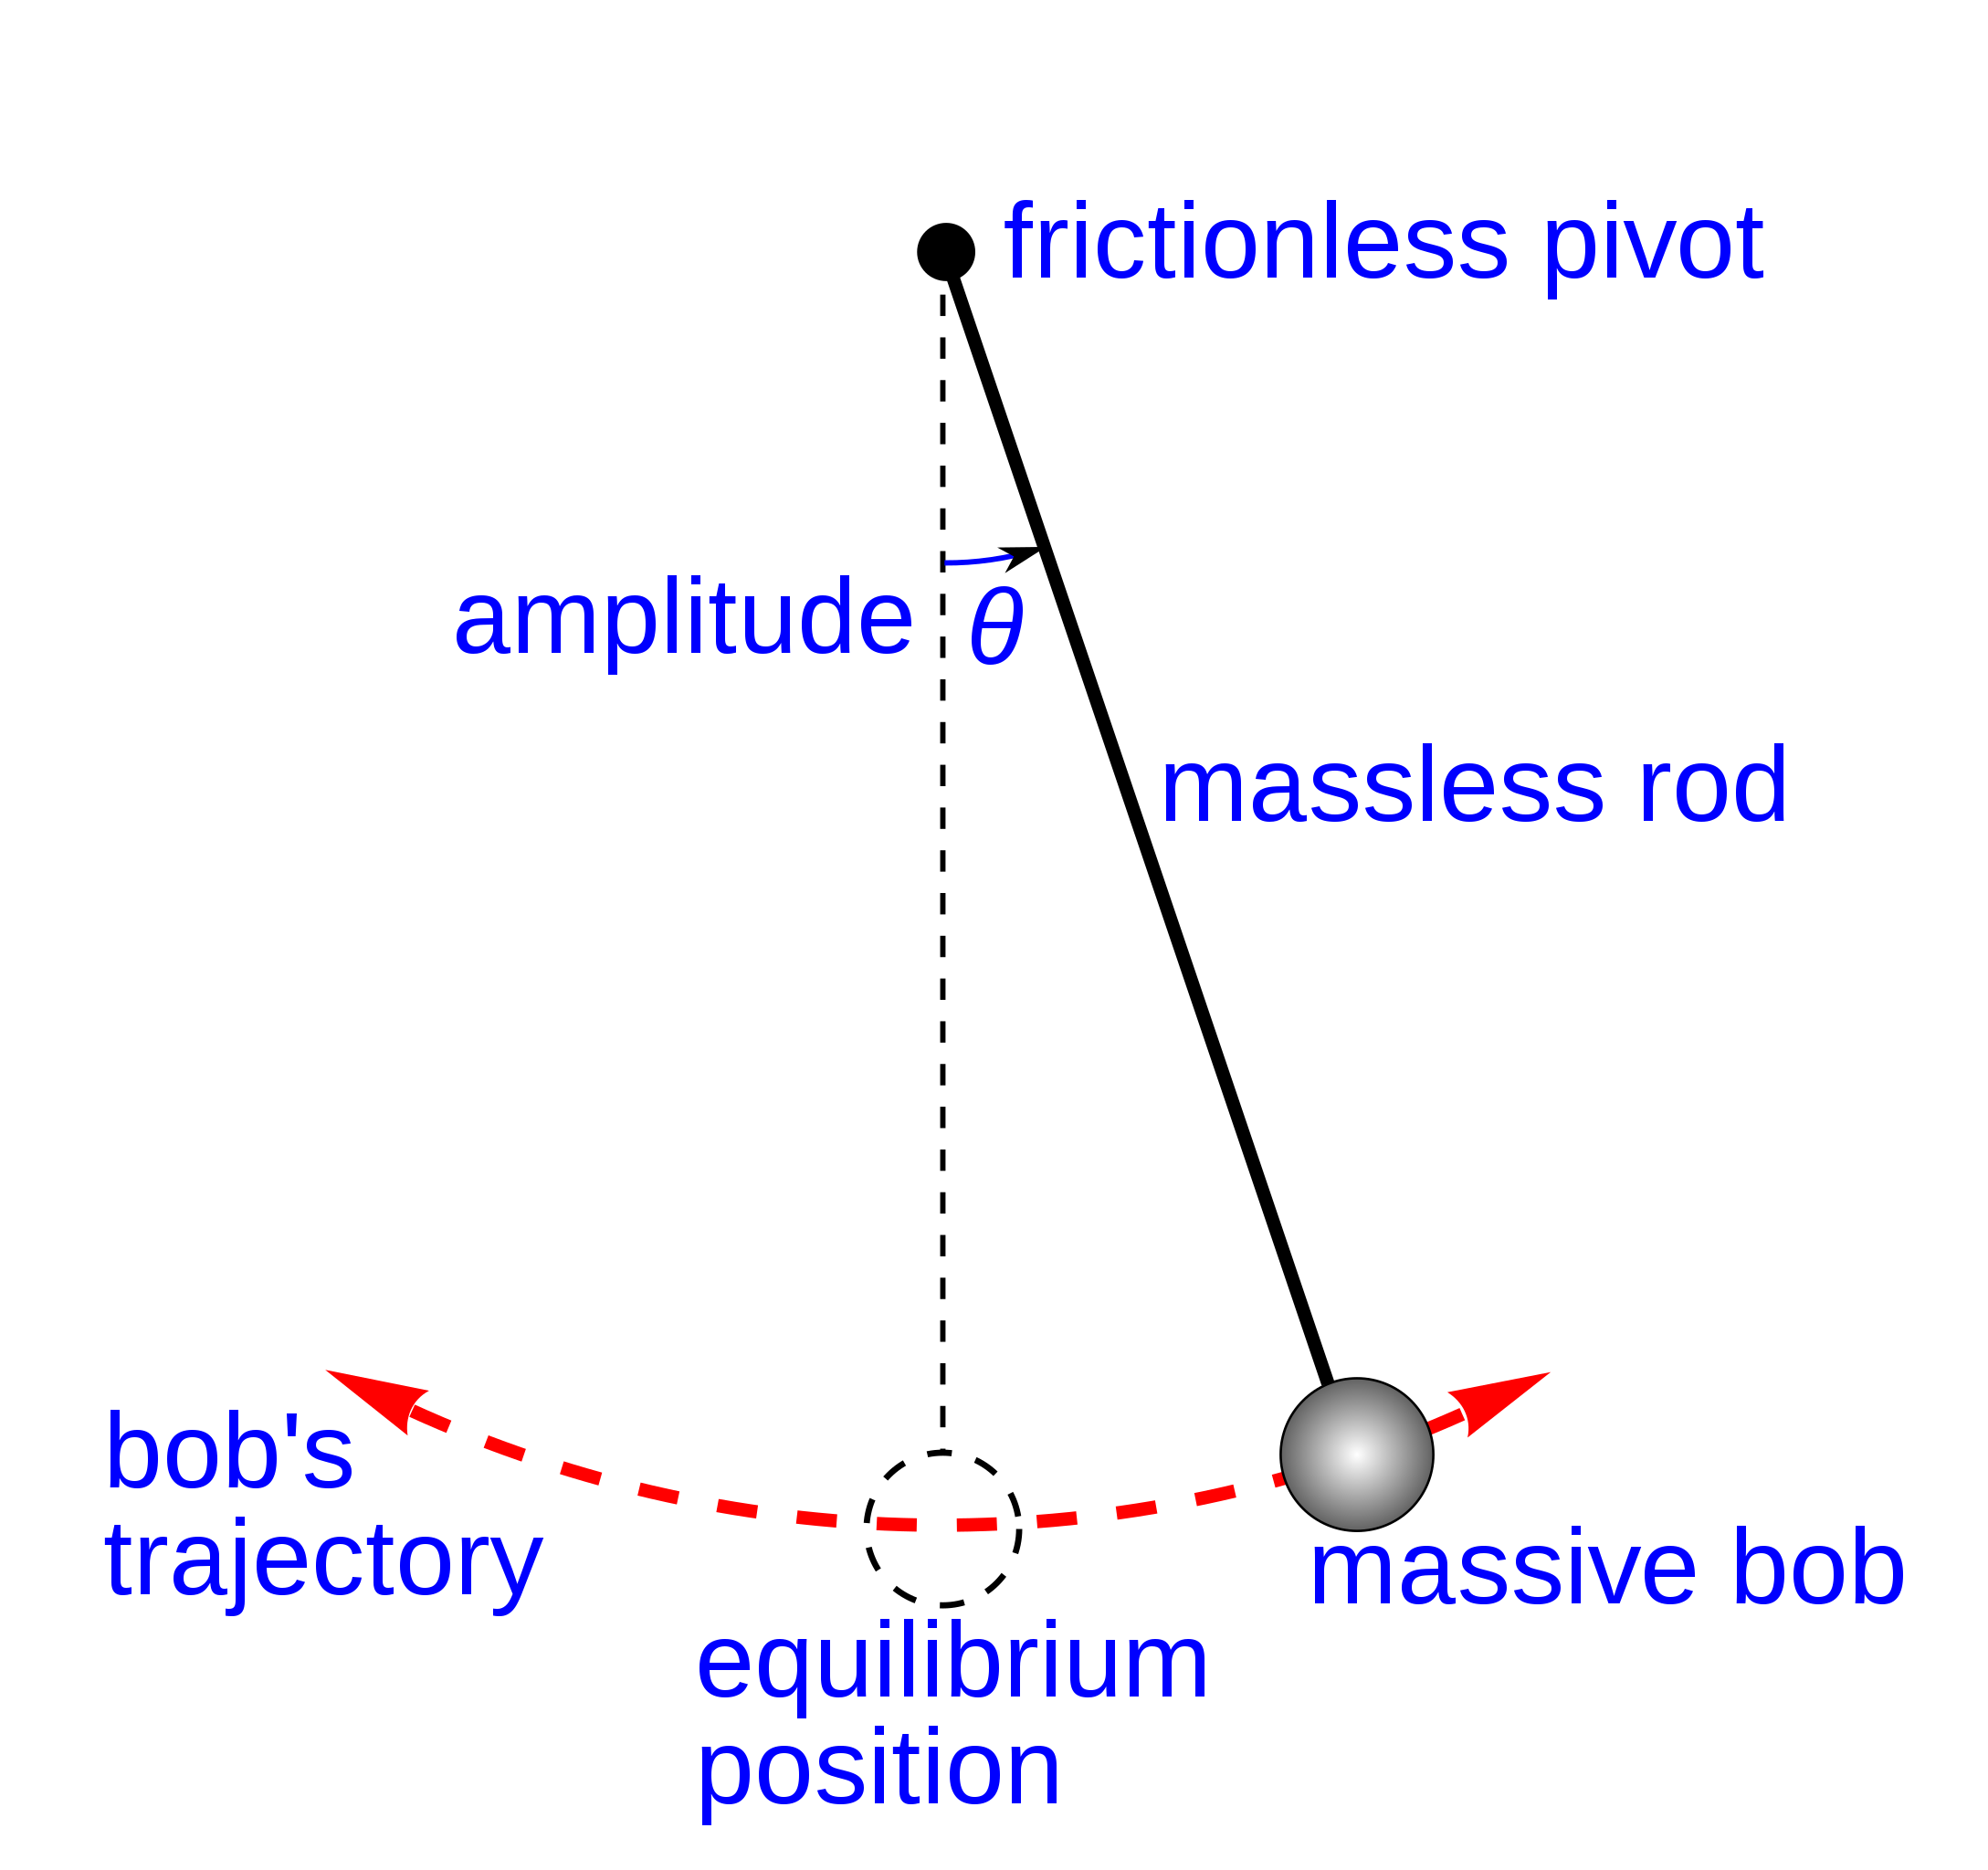
\includegraphics[width=0.6\textwidth]{figures/Simple_gravity_pendulum.png}
   %}{A schematic of the simple pendulum}
    \caption{A schematic of the simple pendulum from \href{https://commons.wikimedia.org/wiki/File:Simple_gravity_pendulum.svg}{Wikimedia Commons}.}
    \label{fig: simple pendulum}
\end{figure}


\paragraph{The simple pendulum:}  The other common example of simple harmonic motion is the \textbf{simple pendulum}. The basic set up is shown in \cref{fig: simple pendulum} and consists of a bob of mass $m$ on the end of a massless rod, or piece of string, of length $l$, we will also be making the assumption that the angular displacement $\uptheta$ is small\footnote{As the initial angle $\uptheta$ determines the amplitude we sometimes refer to $\uptheta$ itself as the amplitude. }. This is called a simple pendulum as it is a first approximation to the motion of a pendulum, it can be made more sophisticated by dropping the assumption that the the rod is massless and by considering initial displacements where the angle $\uptheta$ is large. We will not be very specific about what ``large'' means for $\uptheta$. However, in the lab sessions you will want to keep $\uptheta$ less than $20^{\circ}$ to be in this regime. Note that while I have given $\uptheta$ in degrees here we will need to work in radians for most of the mathematical expressions given in this section to be valid.\\

Equilibrium for this system is when the string hangs vertically downwards and with the tension in the string balancing the weight of the mass. If we displace the mass from equilibrium it will oscillate around its lowest point. In this case the restoring force is given by the horizontal component of the weight. The horizontal and vertical components are:
\begin{align*}
F_{\text{perp}}&=mg\cos\uptheta,\\
F_{\text{par}}&=-mg\sin\uptheta.
\end{align*}

\begin{figure}[ht]
    \centering
    \ThisAltText{ A triangle showing how the weight of the pendulum bob is decomposed into components.}
   % \pdftooltip{
   \begin{tikzpicture}[scale=2]
  \coordinate [label=left:$\theta$] (C) at (-1.5cm,-1.cm);
  \coordinate (A) at (1.5cm,-1.0cm);
  \coordinate (B) at (1.5cm,1.0cm);
  \draw (C) -- node[left] {$F_{W}=mg$} (B) -- node[right] {$mg\cos\uptheta$} (A) -- node[below] {$mg\sin\uptheta$} (C);
  \draw (1.25cm,-1.0cm) rectangle (1.5cm,-0.75cm);
  \tkzMarkAngle[size=1cm,color=blue](A,C,B)
 % \tkzMarkAngle[size=1cm,color=blue](C,B,A)
\end{tikzpicture}
%}{Components of the weight}
    \caption{The weight of the pendulum bob and its components. \textcolor{red}{This figure needs improved.}}
    \label{fig: weight components}
\end{figure}

The restoring force is thus $-mg\sin\uptheta$, while the tension in the rod balances the perpendicular component $F_{\text{perp}}$.  The restoring force leads to an acceleration through Newton's second law,
\begin{equation*}
a=\frac{F}{m}=-\frac{mg\sin\uptheta}{m}=-g\sin\uptheta.
\end{equation*}
When the angle is small we can use the approximation $\sin\uptheta\sim\uptheta=\frac{s}{l}$, where $s$ is the arc length. This means that
\begin{equation*}
a=-\frac{g}{l}s,
\end{equation*}
which is shm with an angular frequency of 
\begin{equation}
\upomega^{2}=\frac{g}{l},
\label{eq: pendulum frequency}
\end{equation}
and the period of oscillation is
\begin{equation}
T=\frac{2\uppi}{\upomega}=2\uppi\sqrt{\frac{l}{g}}.
\label{eq: pendulum period}
\end{equation}
Notice that unlike with a spring gravity is important.\\

As an aside note that we can think of the simple pendulum as being a ``spring'' with a mass dependent spring constant, $k_{\text{eff}}=\frac{mg}{l}$. This is related to an approximation scheme that is very common in physics where we use a a simple harmonic oscillator as a model for the low energy behaviour of many different phenomena.\\

Another point to be aware of is that the approximation that we used above, $\sin\uptheta\sim\uptheta$, is just the first term in what is known as a Taylor expansion where we can expand the $\sin$ function as
\begin{equation*}
\sin\uptheta=\uptheta-\frac{\uptheta^{3}}{3!}+\frac{\uptheta^{5}}{5!}-\dots, \qquad \text{for all } \uptheta.
\end{equation*}
If we want to understand the physics of a pendulum for angles larger than $10^{\circ}$ to $20^{\circ}$ more terms need to be included. This approximation is valid in both degrees and radians, however, if we then go on and use that $\uptheta=\frac{s}{l}$ in terms of the arc length, this is only valid if $\uptheta$ is measured in radians.\\

The expression for the period of the pendulum in \cref{eq: pendulum period} shows that the period can be changed by lengthening the string of pendulum rod. As mentioned above, the period would also change if the pendulum was set up on a planet with different gravity.\\

We can analyse oscillations by considering how the types of energy change during the motion. In particular, for a pendulum at its maximum displacement the bob is instantaneously at rest, since the motion is changing direction, and all of the energy is potential. While when the pendulum bob is passing through equilibrium all of the energy is kinetic.\\

In general the potential energy of a spring is
\begin{equation*}
E_{P}=\frac{1}{2}kx^{2},
\end{equation*} 
where $x$ is the displacement from equilibrium. Since at the maximum amplitude, $x=A$ all of the energy is potential, the total energy is
\begin{equation*}
E=\frac{1}{2}kA^{2}.
\end{equation*}
Since the total energy is $E_{K}+E_{P}$ the kinetic energy of the spring can be expressed as
\begin{equation*}
E_{K}=\frac{1}{2}\left(A^{2}-x^{2}\right).
\end{equation*}

We can use this to find a linear speed\footnote{As in this is the speed that the object has is we think of it as a moving in one dimension.} for the object at a displacement of $x$ from equilibrium. To do this write $E_{K}=\frac{1}{2}mv^{2}$ and equate the two expressions for the kinetic energy:
\begin{align*}
\frac{1}{2}mv^{2}&=\frac{1}{2}k\left(A^{2}-x^{2}\right),\\
\Rightarrow \, v^{2}&=\frac{k}{m}\left(A^{2}-x^{2}\right)=\upomega^{2}\left(A^{2}-x^{2}\right),
\end{align*}
which means that
\begin{equation*}
v=\pm\upomega\sqrt{A^{2}-x^{2}}.
\end{equation*}
Note that this fits our intuition that the velocity should be maximum at equilibrium where $x=0$, and zero at the maximum displacement, $x=\pm A$. If we plot both $E_{K}$ and $E_{P}$ we see that they are both parabolas, and the total energy is just a straight line. \textcolor{red}{This figure needs to be added.}

\section{Damping, Forcing, and Resonance}
So far we have studied oscillating objects while ignoring friction, air resistance, and any other force which may cause the oscillations to gradually die away. These are known as dissipative forces, and are essential when trying to match up our idealised models of oscillators with how real oscillators behave. We call the motion \textbf{damped} if there are dissipative forces. If we ant to make our models realistic we have to consider these dissipative effects along with phenomena like forcing and resonance. This section of the module is much more qualitative than the others. It can be made quantitative but the full mathematical description is more advanced than we want to be concerned with in this module. If you go on to study more physics during your degree then you will likely get to learn more about the maths behind these phenomena. If you want to know more now, then you can ask in the lectures or take a look at the further reading suggestions. \\

There are three types of damping that we are interested in here.
\begin{itemize}
\setlength{\itemsep}{-5pt}
    \item \textbf{Light damping:} This is when the time period is independent of the amplitude so each cycle of oscillation takes the same time, but the amplitude is gradually decreasing as the oscillations die away. 
    \item \textbf{Critical damping:} There is just enough damping to stop the system from oscillating after it has been displaced. This type of damping returns the oscillating object to equilibrium by the shortest possible route.
    \item \textbf{Heavy damping:} This occurs when the damping is so strong that no oscillating motion occurs and the mass returns to equilibrium straight away, but by a much slower route than for critical damping.
\end{itemize}  

\paragraph{Example 7.5:} Consider the following cases of damping and decide if they are light, critical, or heavy:
\begin{itemize}
\setlength{\itemsep}{-5pt}
    \item[a)] A child on a swing displaced from equilibrium and then released,
    \item[b)] A car suspension system,
    \item[c)] The door closer on a fire door.
\end{itemize}  

a) This is lightly damped as the swing will keep oscillating with the amplitude gradually decreasing as it returns to equilibrium. \\

b) Suspension is critically damped as we want the car to return to equilibrium as quickly as possible to avoid throwing the passengers around.\\

c) This is heavily damped as there are no oscillations, the closer ensures that the door returns to equilibrium, closed, in a slow and gentle manner.\\


As well as considering dissipative forces that damp an oscillator we can imagine adding forces that drive the oscillator. Imagine pushing someone on a swing, we are applying an external force, the push, to drive the motion of the oscillator rather than just displacing them from equilibrium and leaving them to oscillate back and forth. If we time our pushes well then they make the sing go higher and higher. This is known as \textbf{driving} or \textbf{forcing} the oscillation since we are applying an external force. These pushes are a periodic force, eg a force applied at regular intervals. When there is no external periodic force being applied we say that an oscillating system is oscillating at its \textbf{natural frequency}. When a periodic force is applied, we call it a \textbf{forced vibration}. In this case the response, ie the oscillation frequency, depends on the frequency of the forcing.\\

Consider forcing a spring, we could do this by just stretching and compressing the spring by hand, the frequency of oscillation is the applied frequency. A natural question is ``what happens if the applied frequency is increased?'' 

As the applied frequency increases from zero we would notice a few things happening. First, the amplitude of oscillation will initially increase, until it reaches some maximum amplitude at a particular applied frequency before starting to decrease as the frequency continues to be raised. The phase difference between the displacement of the oscillating object and the applied force increases from $0$ to $\uppi/2$, reaching $\uppi$ when the amplitude reaches its maximum value. The phase difference will then keep increasing up to $\uppi$ as the applied frequency is increased further. It would then keep increasing up to a phase difference of $2\uppi$ which is equivalent to a difference of $0$.\\

When the system is oscillating with its maximum amplitude, the phase difference between the driving force and the displacement is $\uppi/2$. This means that the driving force is in phase with the oscillators velocity and we say that the system is in \textbf{resonance}. The frequency at the maximum amplitude is called the \textbf{resonant frequency}. The lighter the damping the larger the maximum amplitude is at resonance and the closer that the resonant frequency is to the natural frequency. If there is no damping then the maximum amplitude would diverge at resonance, in practice this means that systems break when they reach resonance. On the other hand, if the damping is large enough then resonance can essentially be removed entirely. A famous example is the collapse of the Tacoma bridge. With a bridge like this we model it on an oscillator since it can be springy and bounce when someone walks across it. Most bridges are fitted with dampers so that resonance is avoided, this is very important since the steps of people walking across the bridge act like a periodic driving force.\\


%%%%%%%%%%%%%%%%%%%%%%%%%%%%%%%%%%%%%%%%%%%%%%%%%%%%%%%%%%%%%%%%%%%%%%%

\chapter{Electric Circuits}
The penultimate section of this module changes tack and explores the basic physics of electric circuits and their components. \textcolor{red}{This section involves lots of pictures some of which will be added in later, initially it may be hard to read parts of this section and you should use the handwritten lecture notes to see the relevant figures.}

\section{Voltage, Current, and Resistance}
\paragraph{Current:} Electricity is the flow of charge around a circuit, this is known as an \textbf{electrical current}. Usually we are thinking of a flow of electrons\footnote{Fundamental particles that carry a negative electrical charge.}, but these could also be positively charged protons or charged ions. We call the particles flowing round the circuit \textbf{charge carriers}.\\

By convention we say that a \textbf{current} flows from a positive charge to a negative charge\footnote{I believe that we can blame Benjamin Franklin for picking this convention and it is now so ingrained that nobody is campaigning to change it.}, even if the charge carriers are travelling in the opposite direction. This means that in an electrical circuit the current is in the opposite direction to the flow of electrons.\\

If we look at a battery, which is often called a \textbf{cell} in electronics, the two ends of the battery are marked with a $+$ and a $-$, we call these ends terminals and when we connect wires to the battery we can think of electrons as flowing from the $-$ terminal through the wire, and anything else that is connected to it, and then going back into the $+$ terminal. A current will only flow if  the circuit is closed, if there are any breaks then a current will not flow.\\

Current is give the symbol $I$ and is measured in Amperes, often shortened to Amps\footnote{Named after Andr\'{e}-Marie Amp`{e}re.}, with the symbol $\text{A}$.\\

There are two types of circuit that we care about in this module:
\begin{itemize}
\setlength{\itemsep}{-5pt}
    \item \textbf{Direct Current:} This is where a cell produces a constant current which points in the same direction, this is the case where our cartoon picture of a flow of electrons makes sense.
    \item \textbf{Alternating Current:} The voltage and current in a circuit are periodic and change direction in time. In this case the picture is more like the electrons in the wires are oscillating backwards and forwards. We will study AC circuits at the end of this section where we will make use of a lot of the ideas about periodicity and circular motion that we met earlier in the module.
\end{itemize}  

We can formalise some of the concepts that were introduced above. \textbf{Charge}\footnote{Here we use charge and electric charge synonymously, however there are other types of charge that show up in other contexts. For example mass can be thought of as being gravitational charge since it quantifies how an object responds to a gravitational field.}, given the symbol $Q$, is a property of an object which determines how the object responds to an electromagnetic field. Charge is measured in units called Coulombs\footnote{These are named after Charles-Augustin de Coulomb.} and given the symbol $\text{C}$. We said above that a current is a flow of charge carriers and this leads us to relate Coulombs to Amps through $1\text{C}=1\text{A}s$ ie one coulomb is one Amp in one second. Alternatively we can write this as
\begin{equation}
I=\frac{\Delta Q}{\Delta t},
\label{eq: current definition}
\end{equation}
or in words, current is the rate of change of charge.\\

An electron has a tiny charge of $Q=1.6\time10^{-19}\text{C}$, so a current of $1\text{A}$ is due to $6.25\times 10^{18}$ electrons passing along the wire per second. Note that we have not put a minus sign on the charge of an electron, in many places you will see it quoted as $q_{e}=-1.6\time10^{-19}\text{C}$, but we are not that concerned with what the charge carriers are in this module so have quoted the charge without a sign in this case.\\

In terms of how they respond to electrical currents physical materials essentially come in three types:
\begin{itemize}
\setlength{\itemsep}{-5pt}
    \item \textbf{Conductors:} These have free charge carriers and allow a current to flow through them. The wire used to connect circuit components in the lab is an example of a conductor.
    \item \textbf{Insulators:} These do not support conduction of electricity. Think of materials like rubber, wood, or plastic.
    \item \textbf{Semiconductors:} These are a halfway house where the conduction properties depend on what we do to the material, for example they can depend on the temperature with certain materials being insulators at low temperatures and becoming conductors as they heat up. The physics of semiconductors is complicated, but they are integral to many modern technologies.
\end{itemize}  

The important points to remember are that a current delivers energy around the circuit, and the cell or battery has the potential to transfer its chemical energy to the kinetic energy of the charge carriers.

\paragraph{Example 8.1:}What is the current if $10\text{C}$ of charge passes along a wire in $10\text{s}$?\\

Use $I=\frac{Q}{t}$ and substitute in the numbers given in the question:
\begin{equation*}
I=\frac{10}{10}=1\text{A}.
\end{equation*}

A very useful analogy to have in mind when thinking about electric circuits is of water flowing through pipes. The flow of water is like the flow of charge carriers and the rate that water flows at is the current.  We can then ask what cells or batteries would be in this analogy? The answer is that these are like the water starting off at the top of a hill where it has potential energy, and as it flows through the circuit this potential energy is converted into the kinetic energy of the charge carriers. Then when charge carriers pass through a circuit component this is like a water fall where the water loses potential energy as it falls.\\


\paragraph{Voltage:} More formally, each charge carrier does work when it passes through a component. This work done is equal to a loss of energy of the charge carriers. Since in our analogy this would be a loss of potential energy as the water falls, we refer to the drop in energy across a component as the \textbf{potential difference}.

\begin{equation*}
\text{Work done per charge} = \text{Potential Difference (pd)} = \text{Voltage}.
\end{equation*}
The terms potential difference and voltage are used essentially interchangeably  and both are measured in units of Volts, $\text{V}$, with $1\text{V}=1\text{J/C}$. 

\paragraph{Example 8.2:} If $30\text{J}$ of work is done when $5\text{C}$ of charge passes through a circuit component, find the voltage.\\

We are told both the charge and the work done so can use
\begin{equation*}
V=\frac{W}{Q}=\frac{30}{5}=6\text{V}.
\end{equation*}

The voltage supplied by a cell or battery is often called the \textbf{electromotive force} or EMF and is given the symbol $\mathcal{E}$. We saw above that voltage was a measure of the energy per charge, this means that the product of voltage and charge is a measure of energy. In other words
\begin{equation}
\text{Electrical Energy}=E=\mathcal{E}Q,
\end{equation}
where here electrical energy means the energy supplied to the circuit by the cell.\\

In our water analogy, the electrical energy is like the initial potential energy determined by the height that the water starts of at. This energy will decrease every time we pass through a circuit component as that is analogous to the water going down a drop and turning some of its potential energy into kinetic energy, heat energy, or sound.\\

Charge carriers lose energy when they pass through circuit components like bulbs as their energy is used to make the component work, ie light up in the case of a bulb. However, they will also lose energy as they pass through the wires in a circuit, since the cause the wire to heat up slightly. This is known as \textbf{resistance}, and we normally ignore the resistance of the wires in a circuit as it is so much smaller than the resistance of the circuit components. In the water analogy, the resistance is like the width of the pipe. If a pipe narrows this slows down the flow of water and reduces its kinetic energy.\\

Certain circuit components like resistance heaters and filament bulbs have high resistances. In fact a filament bulb is more of a heater than a light, it only produces light as a by-product of the filament heating up.\\

Combining all of the ideas we have seen so far, consider a circuit component with a potential difference $V$ across it and a current $I$ passing through it for a time $t$ We can then compute the charge that flows through the component in that times $Q=It$ and the work done by the charges is
\begin{equation*}
W=QV=ItV,
\end{equation*}
but we know that Power is work divided by time, so we get a measure of electrical power from
\begin{equation*}
P=\frac{W}{t}=IV.
\end{equation*}

This is another equation you can use a formula triangle to help you remember, see \cref{fig: PIV triangle}.   When you buy a bulb in a shop the power rating corresponds to the electrical power that needs to be supplied for the bulb to illuminate. As in the case of mechanical power we use Watts, $\text{W}$, as the unit of power.

\begin{figure}[ht]
    \centering
    \ThisAltText{ The formula triangle for power, voltage, and current.}
  %  \pdftooltip{
  \large \formulatriang[.4]{$P$}{}{$I$}{}{$ V$}{}
  %}{The formula triangle for power, voltage, and current.}
    \caption{The formula triangle for power, voltage, and current. }
    \label{fig: PIV triangle}
\end{figure}


\paragraph{Example 8.3:} A $6\text{V}$, $12\text{W}$ bulb is connected to a $6\text{V}$ battery. Calculate:
\begin{itemize}
\setlength{\itemsep}{-5pt}
    \item[a)] The current through the bulb,
    \item[b)] The energy transferred to the bulb in $1800\text{s}$.
\end{itemize}  
Note that when we quote a voltage associated with a circuit component we mean that this is the potential difference needed for the component to work.\\

a) Use $P=IV$ and rearrange it to give
\begin{equation*}
I=\frac{P}{V}=\frac{12}{6}=2\text{A}.
\end{equation*}

b) We know that $E=Pt$ so can substitute in $P$ and $t$ to calculate
\begin{equation*}
E=Pt=12\times 1800=21600\text{J}\simeq 22\text{kJ}.
\end{equation*}


\paragraph{Resistance:} The resistance is a measure of how difficult it is to make a current flow through a circuit component. At a microscopic level we can think of it as being caused by collisions between the charge carriers. It is given as the ration of the voltage across a component to the current passing through it and we give it the symbol $R$. The unit of resistance is the Ohm\footnote{After Georg Ohm.} $\Omega$.\\

This relationship between voltage, current, and resistance is known as Ohm's law and is not true for every material, in fact we call materials where Ohm's law holds Ohmic materials. Unless explicitly stated, in this module we are assuming that all materials are Ohmic. As in the case of Hooke's law, Ohm's law describes how a material behaves under certain conditions, if we put too big a current or too high a voltage through a material we can find that Ohm's law will break down above a certain point. As an equation Ohm's law is
\begin{equation}
V=IR.
\label{eq: Ohms law}
\end{equation}
The formula triangle in \cref{fig: Ohms law} can help you remember how to rearrange Ohm's law. This relationship shows us how to define the Ohm as a unit with $1\Omega=1\text{V/A}$.

\begin{figure}[ht]
    \centering
    \ThisAltText{ The formula triangle for voltage, current, and resistance.}
   % \pdftooltip{
   \large \formulatriang[.4]{$V$}{}{$I$}{}{$ R$}{}
   %}{The formula triangle for Ohm's law.}
    \caption{The formula triangle for Ohm's law. }
    \label{fig: Ohms law}
\end{figure}

One of the lab experiments involves you testing a circuit component called a resistor and checking that Ohm's law is satisfied for this component. A consequence of \cref{eq: Ohms law} is that if we plot voltage against current, for a material where Ohm's law is valid, we will get a straight line graph whose gradient is the resistance.

\paragraph{Example 8.4:} The current through a circuit component is $2\text{mA}$ when the potential difference is $12\text{V}$. Calculate:
\begin{itemize}
\setlength{\itemsep}{-5pt}
    \item[a)] Its resistance,
    \item[b)] The voltage across the component if the current is $50\mu\text{A}$.
\end{itemize}

a) Use Ohm's law to write $R=V/I$ and substitute in the numbers that we are given:
\begin{equation*}
R=\frac{V}{I}=\frac{12}{0.0002}=6000\Omega = 6\text{k}\Omega.
\end{equation*}

b) Resistance is a property of a material so remains constant, unless we are told that the material has special properties where its resistance depends on the temperature or on the light level. We have changed $I$ and are keeping $R$ fixed so can use Ohm's law to find $V$ through
\begin{equation*}
V=IR=50\times10^{-6}\times 6\times 10^{3}=0.3\text{V}.
\end{equation*}


There is a special circuit component, called a \textbf{resistor}, whose purpose is just to add particular resistance to a circuit. In one of the lab sessions you will look at several resistors in a circuit and test Ohm's law by measuring the voltage across all of the resistors.  There are two circuit symbols that re used to stand for a resistor, both are shown in \cref{fig: resistors}.

\begin{figure}[ht]
    \centering
    \ThisAltText{ The circuit symbols for a resistor.}
   % \pdftooltip{
   \begin{tikzpicture}[circuit ee IEC]
    % Var resistor
  \begin{scope}[set resistor graphic=var resistor IEC graphic]
    \draw (0,1) to [resistor] (2,1);
    % Back to original
    \draw [set resistor graphic=resistor IEC graphic]
      (0,0) to [resistor] (2,0);
  \end{scope}
\end{tikzpicture}
%}{resistors}
    \caption{The two symbols for a resistor in a circuit}
    \label{fig: resistors}
\end{figure}

A natural question after what we have seen in this section is ``How do we measure current and voltage?'' The answer is that there are two specific circuit components that we add to a circuit to do this. To measure the current through a circuit we connect a device called an \textbf{ammeter} into the circuit as shown in \cref{fig: ammeter}.

\begin{figure}[ht]
    \centering
    \ThisAltText{ The circuit symbol for an ammeter which is connected in series with the component that you are measuring the current through.}
    %\pdftooltip{
    \begin{tikzpicture}[circuit ee IEC]
     \draw (0,0) to [battery] (4,0) ;
    \draw (0,-2) to [amperemeter] (2,-2);
    \draw    (2,-2) to [resistor] (4,-2);
    \draw (0,0) to (0,-2);
    \draw (4,0) to (4,-2);
\end{tikzpicture}
%%}{ammeter}
    \caption{An ammeter is connected in series to measure the current through a circuit.}
    \label{fig: ammeter}
\end{figure}

Voltage is measured using a different device called a \textbf{voltmeter}, which is connected across a circuit component, rather than  being inserted beside the resistor. This is shown in \cref{fig: voltmeter}. In the next subsection we will learn about why these two circuits look different. We say that the ammeter and resistor are in series while the voltmeter and resistor are in parallel. If you look in an older book you may find a generic meter being referred to as a \textbf{galvanometer}, this is a device that can be set up to measure current or voltage, it can even be used to measure resistance. 

\begin{figure}[ht]
    \centering
    %\pdftooltip{
    \ThisAltText{ The circuit symbol for a voltmeter which is connected in parallel to the component that you are measuring the voltage across.}
    \begin{tikzpicture}[circuit ee IEC]
     \draw (-1,0) to [battery] (3,0) ;
    \draw (0,-4) to [voltmeter] (2,-4);
    \draw    (-1,-2) to [resistor] (3,-2);
    \draw (0,-2) to (0,-4);
    \draw (2,-2) to (2,-4);
    \draw (-1,0) to (-1,-2);
    \draw (3,0) to (3,-2);
\end{tikzpicture}
%}{voltmeter}
    \caption{A voltmeter is connected in series to measure the voltage across a circuit component.}
    \label{fig: voltmeter}
\end{figure}

\section{Series and Parallel Circuits}
It turns out that there are a set of rules that govern how current and voltage behave in a circuit. These are known as \textbf{Kirchhoff's laws}\footnote{Named for Gustav Kirchhoff}, and understanding how an electric circuit will behave is often just a case of applying these rules. It is natural to separate these rules into the current laws and the voltage laws, when we state these it should become clear why we connect ammeters and voltmeters in different ways as that comes from these rules. \\

\paragraph{Current rules:} There are two current rules.
\begin{itemize}
\setlength{\itemsep}{-5pt}
    \item[1)] When multiple wires meet at a junction the total current entering the junction is equal to the total current leaving the junction. As an example consider the diagram in \cref{fig: K1}. Here the current rule says that $1.5\text{A}=0.5\text{A}+I$ which means that $I=1\text{A}$ going in to the junction.
    \item[2)] For components in series, ie components that are side by side, the current entering a component is equal to the current leaving a component. So in the \cref{fig: K2} below the reading on both ammeters will be the same.
\end{itemize}
   \begin{figure}[ht]
    \centering
   % \pdftooltip{
   \ThisAltText{ Kirchhoff's first law that the current entering a junction must be equal to the current leaving the junction.}
   \begin{tikzpicture}[circuit ee IEC]
   \draw (0,0) to[current direction={near start,info={$0.5$A}}] (2,0);
     \draw (3,-1) to[current direction={near start,info={$I=?$}}] (2,0);
        \draw (2,0) to[current direction={near end,info={$1.5$A}}] (3,1);
\end{tikzpicture}
%}{Current rule 1}
    \caption{The current entering the junction is equal to the current leaving the junction.}
    \label{fig: K1}
\end{figure}

 \begin{figure}[ht]
    \centering
   % \pdftooltip{
   \ThisAltText{ The current entering a circuit component is the same as the current leaving it.}
   \begin{tikzpicture}[circuit ee IEC]
   \draw (-1,0) to [battery] (3,0) ;
    \draw    (-1,-2) to [bulb] (3,-2);
    \draw (-1,0) to [amperemeter] (-1,-2);
    \draw (3,0) to [amperemeter] (3,-2);
\end{tikzpicture}
%}{Current rule 2}
    \caption{The current entering a circuit component is the same as the current leaving it.}
    \label{fig: K2}
\end{figure}

The second current rule can also be interpreted as saying that for components in series the current passing through them is the same. If we have components in parallel then we need to use rule 1) to say how the current splits up at the junction.

\paragraph{Voltage rules:} There are three voltage rules. Before stating them it is useful to recall that the voltage between two points in a circuit is equal to the energy transfer per coulomb of charge flowing between the two points.  For example in \cref{fig: voltage rule 0} we have two circuit components that we can consider the potential difference across. 

\begin{figure}[ht]
    \centering
    \ThisAltText{ The voltage across components in parallel is the same.}
   % \pdftooltip{
   \begin{tikzpicture}[circuit ee IEC]
     \draw (-1,0) to [battery] (3,0) ;
    \draw (-1,-4) to [resistor] (3,-4);
    \draw    (-1,-2) to [bulb] (3,-2);
    \draw (-1,-2) to (-1,-4)node[left]{c};
    \draw (3,-2) to (3,-4)node[right]{d};
    \draw (-1,0) to (-1,-2)node[left]{a};
    \draw (3,0) to (3,-2)node[right]{b};
\end{tikzpicture}
%}{voltage across the bulb and resistor agree}
    \caption{$V_{ab}$= voltage across the bulb and $V_{cd}$= voltage across the resistor}
    \label{fig: voltage rule 0}
\end{figure}

If the charge carriers gain energy then there will be a potential rise, such as in a cell. While if they lose energy then there is a potential drop. For most circuit components there will be a potential drop as the charge carriers do work on the circuit component.\\

Kirchhoff's three voltage rules are:

\begin{itemize}
\setlength{\itemsep}{-5pt}
    \item[1)] Voltages in series add, so in a circuit with two resistors in series as in \cref{fig: voltage rule 1} the voltage supplied by the cell is equal to the sum of the potential differences across the resistors, or $V_{0}=V_{1}+V_{2}$.
     \begin{figure}[ht]
    \centering
   % \pdftooltip{
   \ThisAltText{ Voltages in series add to give the total voltage across the components.}
   \begin{tikzpicture}[circuit ee IEC]
     \draw (-3,0) to [battery ={info={$V_{0}$}}] (3,0) ;
    \draw (-0,-3) to [resistor={info'={$V_{1}$}}] (3,-3);
    \draw    (-3,-3) to [resistor={info'={$V_{2}$}}] (0,-3);
    \draw (-3,0) to (-3,-3);
    \draw (3,0) to (3,-3);
\end{tikzpicture}
%}{Voltages in series add }
    \caption{Voltages in series add , $V_{0}=V_{1}+V_{2}$.}
    \label{fig: voltage rule 1}
\end{figure}
    \item[2)] Voltages in parallel are the same. So for a circuit with two resistors in parallel as in \cref{fig: voltage rule 2}, the voltage across both resistors is the same, and this is also the same as the voltage supplied by the cell. Or in symbols $V_{0}=V_{1}=V_{2}$.
    \begin{figure}[ht]
    \centering
    \ThisAltText{ Voltages in parallel are the same.}
  %  \pdftooltip{
  \begin{tikzpicture}[circuit ee IEC]
     \draw (-1,0) to [battery ={info={$V_{0}$}}] (3,0) ;
    \draw (-1,-4) to [resistor={info'={$V_{2}$}}] (3,-4);
    \draw    (-1,-2) to [resistor={info'={$V_{1}$}}] (3,-2);
    \draw (-1,-2) to (-1,-4);
    \draw (3,-2) to (3,-4);
    \draw (-1,0) to (-1,-2);
    \draw (3,0) to (3,-2);
\end{tikzpicture}
%}{Voltages in parallel are the same }
    \caption{Voltages in parallel are the same , $V_{0}=V_{1}=V_{2}$.}
    \label{fig: voltage rule 2}
\end{figure}
    \item[3)] For a loop the sum of voltage gains is equal to the sum of voltage loses. This is a version of the conservation of energy as it is saying that for a closed loop the energy that leaves the circuit is equal to the energy that enters the circuit. For the circuit shown in \cref{fig: voltage rule 3} this means that $V_{0}+V_{1}=V_{2}+V_{3}$
       \begin{figure}[ht]
    \centering
    \ThisAltText{ In a closed loop the total voltage gain is equal to the total voltage loss.}
  %  \pdftooltip{
  \begin{tikzpicture}[circuit ee IEC]
     \draw (-1,0) to [battery ={info={$V_{0}$}}] (3,0) ;
    \draw (3,-4) to [battery={info={$V_{1}$}}] (-1,-4);
    \draw (-1,0) to [resistor={info'={$V_{3}$}}] (-1,-4);
    \draw (3,0) to [resistor={info={$V_{2}$}}] (3,-4);
\end{tikzpicture}
%}{Voltages in loops}
    \caption{For a closed loop the total voltage gain is equal to the total voltage loss.}
    \label{fig: voltage rule 3}
\end{figure}
\end{itemize}

\paragraph{Example 8.5:} Consider the circuit shown in \cref{fig: car charging} which describes a car battery being jump started. There are two batteries with an emf and an internal resistance, denoted by the resistors next to the batteries, and two resistors standing for the resistance in the jump leads. Find the current $I$ in the circuit.\\

  \begin{figure}[ht]
    \centering
    \ThisAltText{ A circuit diagram corresponding to jump starting a car.}
 %   \pdftooltip{
 \begin{tikzpicture}[circuit ee IEC]
     \draw (-3,0) to [resistor={info={$R_{1}=2\Omega$}}](0,0);
     \draw (0,0) to [battery ={info={$V_{0}=12$V}}] (3,0) ;
    \draw (3,0) to [resistor={info={$R_{5}=7\Omega$}}] (3,-4);
    \draw (-3,-4) to [resistor={info'={$R_{3}=4\Omega$}}] (0,-4);
    \draw (-3,0) to [resistor={info'={$R_{2}=3\Omega$}}] (-3,-4);
    \draw (0,-4) to [battery ={info'={$V_{4}=4$V}}] (3,-4);
\end{tikzpicture}
%}{charging loop}
    \caption{A circuit describing a car battery being charged. Since the car batteries are oriented oppositely the upper one is a potential gain, while the lower battery is a potential drop as it is being charged.}
    \label{fig: car charging}
\end{figure}

To analyse this circuit we use a combination of the voltage rules and Ohm's Law.  Voltage rule 3 tells us that the sum of the voltage across all of the resistors plus the voltage across the charging battery is equal to $12\text{V}$, or
\begin{equation*}
\begin{split}
12\text{V}=V_{0}&=V_{1}+V_{2}+V_{3}+V_{4}+V_{5}\\
&=R_{1}I+R_{2}I+R_{3}I+4\text{V}+R_{5}I\\
&=2I+3I+4I+4\text{V}+7I\\
&=16I+4\text{V}.
\end{split}
\end{equation*}
Here we have use the second current law to say that the current is the same through all of the resistors, and made use of Ohm's law to convert the voltage across each resistor into the product of $I$ and the resistance. Now we can solve the linear equation for $I$ as
\begin{equation*}
12=16I+4, \quad \Rightarrow \, 16I=8,
\end{equation*}
or $I=1/2=0.5\text{A}$.\\

This example is about as complicated a problem as you can expect to find where we are just building a circuit from batteries and resistors. If you can solve this problem then you will be able to solve pretty much any problem that you are confronted by.

\paragraph{Example 8.6:} Consider the circuit in \cref{fig: 2 resistors}, find the current through the circuit.\\

  \begin{figure}[ht]
    \centering
    \ThisAltText{ A circuit with a single cell and two resistors.}
   % \pdftooltip{
   \begin{tikzpicture}[circuit ee IEC]
     \draw (-3,0) to [battery ={info={$V_{0}=12$V}}] (3,0) ;
    \draw (3,0) to  (3,-4);
    \draw (-3,0) to  (-3,-4);
    \draw (-3,-4) to [resistor={info'={$R_{1}=4\Omega$}}] (0,-4);
    \draw (0,-4) to [resistor ={info'={$R_{2}=8\Omega$}}] (3,-4);
\end{tikzpicture}
%}{A potential divider}
    \caption{A circuit with a single cell and two resistors.}
    \label{fig: 2 resistors}
\end{figure}

This ii similar to the previous example in that we use Ohm's law to convert $R_{1}$ and $R_{2}$ into a voltage through $V_{1}=I R_{1}$ and $V_{2}=I R_{2}$ and then use the second current rule that the total current gained in a closed loop is equal to the total current lost in the loop. In other words:
\begin{equation*}
12\text{V}=V_{1}+V_{2}=\left(R_{1}+R_{2}\right)I=12I,
\end{equation*}
so $I=12/12 \text{A}=1\text{A}$.


\paragraph{Combining resistors:} A consequence of Kirchhoff's laws is that we can now combine all the resistance in a circuit and construct an analogous circuit which has the same total resistance but all of it is contained in one resistor. In fact we can start to see this in the above example where we have 
\begin{equation*}
V_{0}=\left(R_{1}+R_{2}\right)I,
\end{equation*}
from Ohm's law this would be like having a single resistor whose resistance is $R=R_{1}+R_{2}$. \\


This is exactly what happens for resistors in series, their resistance adds. 
\begin{equation}
R=R_{1}+R_{2}.
\label{eq: resistors in series}
\end{equation} 
See \cref{fig: resistance in series} for a what this means in terms of circuit diagrams.\\
  \begin{figure}[ht]
    \centering
    \ThisAltText{ For resistors in series the total resistance is the sum of the individual resistances.}
    %\pdftooltip{
    \begin{tikzpicture}[circuit ee IEC]
    \draw (-3,0) to [resistor={info={$R_{1}$}}] (0,0);
    \draw (0,0) to [resistor ={info={$R_{2}$}}] (3,0);
    \draw (5,0) to [resistor ={info={$R=R_{1}+R_{2}$}}] (8,0);
    \path (3,0) -- (5,0) node[midway, blue]{=};
\end{tikzpicture}
%}{Resistors in Series}
    \caption{Combining resistance in series the resistance adds.}
    \label{fig: resistance in series}
\end{figure}

In the water flowing through pipes analogy, we think of a resistor as being like a drop in height where the water loses potential energy, then this is just saying that if the water drops first a height $h_{1}$ and then a height $h_{2}$, the change in potential energy is the same as if the water dropped a height of $h_{1}+h_{2}$ in one go.\\

Resistors in parallel combine in a more complicated way. This is because we need to use the second voltage rule, that the voltage is the same in parallel paths, and the first current rule, which tells us what happens to the current at a junction. Using both of these we find that if we have two resistors $R_{1}$ and $R_{2}$ in parallel then the combined resistance is
\begin{equation}
\frac{1}{R}=\frac{1}{R_{1}}+\frac{1}{R_{2}}.
\label{eq: resistors in parallel}
\end{equation}

  \begin{figure}[ht]
    \centering
    \ThisAltText{ For resistors in parallel the reciprocal of the total resistance is the sum of the reciprocals of the individual resistances.}
   % \pdftooltip{
   \begin{tikzpicture}[circuit ee IEC]
    \draw (0,0) to [resistor={info'={$R_{1}$}}] (2,0);
    \draw (0,-2) to [resistor ={info'={$R_{2}$}}] (2,-2);
    \draw(0,-1) to[current direction={near start,info={$I_{1}$}}] (0,0);
     \draw(0,-1) to[current direction={near start,info'={$I_{2}$}}] (0,-2);
    \draw (2,0) to[current direction={near start,info'={$I_{1}$}}] (2,-1);
    \draw (2,-2) to[current direction={near start,info={$I_{2}$}}] (2,-1);
    \draw(-2,-1) to[current direction={near start,info={$I$}}] (0,-1);
    \draw(2,-1) to[current direction={near start,info={$I$}}] (4,-1);
    \draw (6,-1)to [current direction={near start,info={$I$}},resistor ={info'={$R=\frac{1}{\frac{1}{R_{1}}+\frac{1}{R_{2}}}$}}] (9,-1);
    \path (4,-1) -- (6,-1) node[midway, blue]{=};
\end{tikzpicture}
%}{Resistors in parallel}
    \caption{Combining resistance in parallel the reciprocals of the resistance add.}
    \label{fig: resistors in parallel}
\end{figure}

What this means for a circuit diagram can be seen in \cref{fig: resistors in parallel}.  From the first current rule we know that $I=I_{1}+I_{2}$ while from the second voltage rule we know that the voltage across resistor 1 is equal to the voltage across resistor 2. If we use Ohm's law on each resistor we have that 
\begin{align*}
V_{1}&=I_{1} R_{1},\\
V_{2}&=I_{2} R_{2},\\
V_{1}&=V_{2}=V.
\end{align*}
While for the single big resistor on the other side we have that $V=IR$.  Then we use the first current rule 
\begin{align*}
I&=I_{1}+I_{2}\\
\frac{V}{R}&=\frac{V_{1}}{R_{1}}+\frac{V_{2}}{R_{2}}\\
&=\frac{V}{R_{1}}+\frac{V}{R_{2}}\\
&=V\left(\frac{1}{R_{1}}+\frac{1}{R_{2}}\right),
\end{align*}
which if we cancel the factors of $V$ gives \cref{eq: resistors in parallel}.

\paragraph{Example 8.7:} Find the combined resistance for the circuit shown in \cref{fig: combining resistance example}. Is it
\begin{itemize}
\setlength{\itemsep}{-5pt}
    \item[a)] $11\Omega$,
    \item[b)] $4\Omega$,
    \item[c)] $1\Omega$.
\end{itemize}

  \begin{figure}[ht]
    \centering
    \ThisAltText{ A circuit with resistors in parallel and in series.}
    %\pdftooltip{
    \begin{tikzpicture}[circuit ee IEC]
    \draw (0,0) to [resistor={info={$R_{2}=3\Omega$}}] (2,0);
    \draw (0,-2) to [resistor ={info'={$R_{3}=6\Omega$}}] (2,-2);
    \draw(0,-1) to (0,0);
     \draw(0,-1) to(0,-2);
    \draw (2,0) to (2,-1);
    \draw (2,-2) to (2,-1);
    \draw(-3,-1) to[resistor ={info'={$R_{1}=2\Omega$}}]  (0,-1);
    \draw(2,-1) to(4,-1);
\end{tikzpicture}
%}{Combining resistance example}
    \caption{Combining resistance for both in series and parallel resistors.}
    \label{fig: combining resistance example}
\end{figure}

The answer is b) $R=4\Omega$. To see this we first combine $R_{2}$ and $R_{3}$ in parallel as
\begin{equation*}
R_{\text{Par}}=\frac{1}{\frac{1}{R_{2}}+\frac{1}{R_{3}}}=\frac{1}{\frac{1}{3}+\frac{1}{6}}=\frac{1}{\frac{1}{2}}=2\Omega.
\end{equation*}
Then we can combine $R_{1}$ and $R_{\text{Par}}$ in series as
\begin{equation*}
R =R_{1}+R_{\text{Par}}=2+2=4\Omega.
\end{equation*}

Note that a) would be the answer if all the resistors were in series, while c) would be the answer if all three were in parallel.

\paragraph{Power:} We saw above that the electrical power through a circuit component is given by $P=IV$. We motivated discussing power by first introducing resistance so it is no surprise that using Ohm's law and $P=IV$ we can express the power in terms of the resistance as either
\begin{equation*}
P=I^{2}R,
\end{equation*}
or
\begin{equation*}
P=\frac{V^{2}}{R}.
\end{equation*}
Remember that the resistance of a component causes the component to heat up, this is how kettles, irons, and filament bulbs work. For these components the power is then the power radiated to the environment by the hot component, either as heat or as light.

\paragraph{Example 8.8:} The potential difference across a $1k\Omega$ resistor is measured to be $6\text{V}$. What is the electrical power supplied to the resistor?\\

We know the voltage and the resistance so can use $P=\frac{V^{2}}{R}$ to calculate that the power is
\begin{equation*}
P=\frac{V^{2}}{R}=\frac{36}{1000}=0.036\text{W}.
\end{equation*}


\paragraph{Potential Dividers:} We saw in Kirchhoff's voltage laws that for resistors in series the potential differences add. This means that combining resistors in series enables us to split the supplied voltage and deliver different voltages across each resistor. A \textbf{potential divider}, sometimes called a voltage divider, is a circuit which makes use of this property. It is a circuit with a cell and two, or more, resistors. If we put other components in parallel to the resistors then by choosing the value of the resistance, we can control the voltage delivered to the component.\\

  \begin{figure}[ht]
    \centering
    %\pdftooltip{
    \ThisAltText{ A potential or voltage divider circuit.}
    \begin{tikzpicture}[circuit ee IEC]
     \draw (-3,0) to [battery ={info={$V_{0}$}}] (3,0) ;
    \draw (3,0) to  (3,-2);
    \draw (-3,0) to  (-3,-2);
    \draw (-3,-2) to [resistor={info'={$R_{1}$}}] (0,-2);
    \draw (0,-2) to [resistor ={info'={$R_{2}$}}] (3,-2);
\end{tikzpicture}
%}{A potential divider}
    \caption{A potential divider circuit with two resistors}
    \label{fig: potential divider}
\end{figure}

A potential divider circuit has the form shown in \cref{fig: potential divider}. The resistors in the circuit can have a fixed resistance, or they can be variable resistors. For fixed resistors, the total resistance in the circuit is $R=R_{1}+R_{2}$, since the resistors are in parallel. Thus Ohm's law gives that the current in the circuit is
\begin{equation*}
I=\frac{V_{0}}{R_{1}+R_{2}}.
\end{equation*}
Using this we can write the potential differences across the resistors as
\begin{align*}
V_{1}&=IR_{1}=\frac{V_{0}R_{1}}{R_{1}+R_{2}},\\
V_{2}&=IR_{2}=\frac{V_{0}R_{2}}{R_{1}+R_{2}}.
\end{align*}

If $R_{1}=5\text{k}\Omega$ and $R_{2}=10\text{k}\Omega$ then
\begin{equation*}
V_{1}=\frac{1}{3}V_{0}, \qquad V_{2}=\frac{2}{3}V_{0},
\end{equation*}
and 
\begin{equation*}
R_{1}=\frac{1}{3}\left(R_{1}+R_{2}\right), \qquad R_{2}=\frac{2}{3}\left(R_{1}+R_{2}\right).
\end{equation*}

Comparing the expression for the voltage and the resistance we see that they are split in the same proportions. ie $V_{1}$ is the same fraction of the supply voltage as $R_{1}$ is of the total resistance. This means that the ratio of voltages is equal to the ratio of resistances:
\begin{equation}
\frac{V_{1}}{V_{2}}=\frac{R_{1}}{R_{2}}.
\label{eq: voltage ratios}
\end{equation}

In a variable potential divider one of the resistors is replaced by a variable resistor, or sliding connection, or a resistor that depends on its surroundings like a thermistor\footnote{The resistance of a thermistor depends on the temperature.} or  light dependent resistor. In this setting as the resistance changes the output voltage across the resistors changes. This is used in devices like volume controls or dimmer switches where we manually adjust the resistance using a dial which changes the output voltage and hence the power being supplied to a bulb.\\

\paragraph{Example 8.9:} Consider the circuit shown in \cref{fig: pd example}.
\begin{itemize}
\setlength{\itemsep}{-5pt}
    \item[a)] Find the current through the circuit,
    \item[b)] Find the voltage across each resistor.
\end{itemize}  
 \begin{figure}[ht]
    \centering
    \ThisAltText{ A specific potential divider circuit.}
   % \pdftooltip{
   \begin{tikzpicture}[circuit ee IEC]
     \draw (-3,0) to [battery ={info={$V_{0}=6\text{V}$}}] (3,0) ;
    \draw (3,0) to  (3,-2);
    \draw (-3,0) to  (-3,-2);
    \draw (-3,-2) to [resistor={info'={$R_{1}=4\Omega$}}] (0,-2);
    \draw (0,-2) to [resistor ={info'={$R_{2}=8\Omega$}}] (3,-2);
\end{tikzpicture}
%}{A potential divider}
    \caption{A potential divider with $R_{1}=4\Omega$ and $R_{2}=8\Omega$.}
    \label{fig: pd example}
\end{figure}

a) As the resistors are in series, add the resistance to give $R=R_{1}+R_{2}=12\Omega$, then use Ohm's law to find the current:
\begin{equation*}
I=\frac{V}{R}=\frac{6}{12}=\frac{1}{2}\text{A}=0.5\text{A}.
\end{equation*}

b) We can compute $V_{1}$ and $V_{2}$ directly using:
\begin{align*}
V_{1}&=\frac{V_{0}R_{1}}{R_{1}+R_{2}}=\frac{6\times 4}{12}=2\text{V},\\
V_{2}&=\frac{V_{0}R_{2}}{R_{1}+R_{2}}=\frac{6\times 8}{12}=4\text{V}.
\end{align*}



\paragraph{Capacitors:} Another type of circuit component that we want to discuss here is a \textbf{capacitor}. This is a circuit component that stores charge its circuit symbol is shown in \cref{fig: capacitor}, and looks very similar to the symbol for a battery.
  \begin{figure}[ht]
    \centering
    %\pdftooltip{
    \ThisAltText{ The circuit symbol for a capacitor.}
    \begin{tikzpicture}[circuit ee IEC]
     \draw (0,0) to [capacitor] (3,0) ;
\end{tikzpicture}
%}{capacitor circuit symbol}
    \caption{The circuit symbol for a capacitor}
    \label{fig: capacitor}
\end{figure}

We can think of a capacitor as being formed from two parallel metal plates separated by some other substance. When the plates are connected to the opposite terminals of a battery the different charges will build up on either plate, so one plate becomes negatively charged and the other becomes positively charged. If the battery is disconnected and an different circuit component is connected across the capacitor then it will discharge all of the stored charges until the plates have become neutral again.\\

It is important to note that a capacitor does not charge instantaneously, it takes time for it to build up charge. Recall that, if the current in a circuit is $I$ then after a time $t$, the amount of charge that has flowed through a circuit component will be $Q=It$, this means that the rate a capacitor charges at depends on the current in the circuit.  The amount of charge that it can build up depends on the potential difference across the capacitor, and a quantity known as the \textbf{capacitance}. Capacitance is measured in Farads\footnote{Named after Michael Faraday.} which have the symbol $\text{F}$. Mathematically capacitance is related to potential difference and charge through
\begin{equation}
C=\frac{Q}{V},
\label{eq: capacitance eq}
\end{equation} 
and $1\text{F}=1\text{C/V}$.\\

One of the lab experiments looks at the charging and discharging times for a capacitor. The key point is that if we have a circuit like that in \cref{fig: RC circuit}, which is known as an RC circuit. If the switch is initially open then the capacitor will start uncharged. Upon closing the switch the capacitor will begin to charge up and after a time $t$ the current in the circuit will be
\begin{equation*}
I(t)=\frac{V_{0}}{R}\exp\left(-\frac{t}{RC}\right),
\end{equation*}
this is time dependent as the more charge that builds up on the capacitor the lower the current being drawn will be, if the capacitor becomes fully charged then current will no longer be able to flow round the circuit. From looking at the expression we see that the capacitor will only become fully charged when $\exp\left(-\frac{t}{RC}\right)=0$, which would need $t\to \infty$. A consequence of this is that the capacitor can become arbitrarily close to being full charged but will never actually reach it.\\

     \begin{figure}[ht]
    \centering
    \ThisAltText{ An RC circuit with a resistor and a capacitor in series.}
    %\pdftooltip{
    \begin{tikzpicture}[circuit ee IEC]
     \draw (-1,0) to [battery ={info={$V_{0}$}}] (3,0) ;
    \draw (3,-4) to [capacitor={info'={$C$}}] (-1,-4);
    \draw (-1,0) to [resistor={info'={$R$}}] (-1,-4);
    \draw (3,0) to [make contact] (3,-4);
\end{tikzpicture}
%}{RC circuit}
    \caption{An RC circuit}
    \label{fig: RC circuit}
\end{figure}
Using this expression for the current we can obtain an expression for the voltage across the resistor
\begin{equation*}
V_{R}(t)=V_{0}\exp\left(-\frac{t}{RC}\right)
\end{equation*}
and by Kirchhoff's voltage laws , the voltage across the capacitor is
\begin{equation*}
V_{C}(t)=V_{0}\left(1-\exp\left(-\frac{t}{RC}\right)\right).
\end{equation*}
Notice that as time goes on the voltage across the resistor drops and the voltage across the capacitor increases.\\
 
A natural time scale is given by $\uptau=RC$ which is known as the \textbf{time constant}. This is the time required for the voltage across the resistor to fall by $V_{0}/e$.\\

If you go on to study more about circuits you will meet the concept of \textbf{impedance} which is a generalisation of resistance that takes account of all of the opposition to the flow of current. This includes contributions from resistance, capacitance, and inductance\footnote{A concept related to a circuit component called an inductor that we will not meet in this module.}.

\section{AC Circuits}
In a DC circuit the supply voltage is a constant in time, usually denoted by  $V_{0}$. While in an AC circuit, the direction the charge carriers move in changes with time. In fact the current is periodic and follows a sinusoidal wave, 
\begin{equation*}
V(t)=V_{0}\sin(\uw t),\qquad I(t)=I_{0}\sin(\uw t),
\end{equation*}
where $\uw=2\up f=2\up/T$ is the angular frequency. As we saw when studying circular motion the frequency is the number of cycles per second and the period $T$ is the time taken for one cycle. In the UK $f=50\text{Hz}$ for mains power.\\

\begin{figure}[ht]
    \centering
    \ThisAltText{ The profile of the voltage in an AC circuit is a sinusoidal curve.}
  %  \pdftooltip{
    \begin{tikzpicture}[domain=0:6.282, smooth,variable=\x]
     \draw[->] (0,0) -- (6.4,0) node[above] {$t$};
  \draw[->] (0,-1.2)node[left] {$-V_{0}$} -- (0,1.2)node[left] {$V_{0}$};
 \draw[color=blue] node[left] {Voltage}  plot (\x,{sin(\x r)}) ;
    \end{tikzpicture}
 %   }{The voltage in an AC circuit }
    \caption{The voltage in an AC circuit is periodic in time.}
        \label{fig: AC voltage}
\end{figure}

We call the amplitude of the current, $I_{0}$, and voltage, $V_{0}$, the \textbf{peak current} and \textbf{peak voltage}. The voltage in an AC circuit is shown in \cref{fig: AC voltage}. The voltage and current in the circuit can be observed by studying an oscilloscope reading of the current or voltage. The frequency $f$ can also be observed using an oscilloscope. What about the power? Recall that $P=IV=I^{2}R$, so the power is also periodic but is given by
\begin{equation*}
P=I_{0}^{2}R\left(\sin\left(\uw t\right)\right)^{2},
\end{equation*}
which is always greater than zero. We call 
\begin{equation*}
\bar{P}=\frac{1}{2}I_{0}^{2}R=\frac{1}{2}P_{0},
\end{equation*}
the mean power, which is half of the peak power $P_{0}$.\\

\begin{figure}[ht]
    \centering
    \ThisAltText{ The profile of the power in an AC circuit is everywhere positive and follows a sinusoidal curve.}
   % \pdftooltip{
    \begin{tikzpicture}[domain=0:6.282, smooth,variable=\x]
     \draw[->] (0,0) -- (6.4,0) node[above] {$t$};
  \draw[->] (0,-2.2) -- (0,4.2);
 \draw[color=blue] node[left] {Power}  plot (\x,{4*sin(\x r)*sin(\x r)}) ;
 \draw[color=red]  plot (\x,{2*sin(\x r)})node[right] {Current} ;
    \end{tikzpicture}
%    }{The power and current }
    \caption{The Power in an AC circuit is related to the square of the current so is everywhere greater than zero.}
        \label{fig: AC Power}
\end{figure}

It is sometimes useful to think about a direct current that produce the same power as the mean power. This current is called the \textbf{root mean squared} current or $I_{\text{rms}}$ and is defined by 
\begin{equation*}
\bar{P}=(I_{\text{rms}})^{2}R=\frac{1}{2}I_{0}^{2}R.
\end{equation*}

This relation means that $I_{\text{rms}}=I_{0}/\sqrt{2}$. It is called the root mean squared current because computing it involves squaring the current, taking its mean, then square rooting this.\\

Similarly for the voltage we have the rms voltage
\begin{equation*}
V_{\text{rms}}=\frac{V_{0}}{\sqrt{2}}.
\end{equation*}
Note that the mean power is given by
\begin{equation*}
\bar{P}=I_{\text{rms}}V_{\text{rms}}.
\end{equation*}

\paragraph{Example 8.10:} Consider an AC source with $f=200\text{Hz}$ and peak current $I_{0}=0.1\text{A}$. Find:
\begin{itemize}
\setlength{\itemsep}{-5pt}
    \item[a)] The period,
    \item[b)] The rms current
\end{itemize}  

a) Use $T=1/f$ so that the period is
\begin{equation*}
T=\frac{1}{f}=\frac{1}{200}=0.005\text{s}=5\text{ms}.
\end{equation*}

b) This time use the expression for $I_{\text{rms}}$ to find:
\begin{equation*}
I_{\text{rms}}=\frac{1}{\sqrt{2}}I_{0}=\frac{0.1}{\sqrt{2}}=0.07\text{A}.
\end{equation*}

\paragraph{Example 8.11:} An alternating current with peak current $I_{0}=3\text{A}$ is passing through a $4\Omega$ resistor. Calculate:
\begin{itemize}
\setlength{\itemsep}{-5pt}
    \item[a)] The rms current,
    \item[b)] The rms voltage across the resistor,
    \item[c)] The peak power,
    \item[d)] The man power.
\end{itemize}  

a) Given $I_{0}=3\text{A}$ then
\begin{equation*}
I_{\text{rms}}=\frac{1}{\sqrt{2}}I_{0}=\frac{3}{\sqrt{2}}=2.12\text{A}.
\end{equation*}

b) Use Ohm's law, $V_{\text{rms}}=I_{\text{rms}}R$ so that
\begin{equation*}
V_{\text{rms}}=I_{\text{rms}}R=\frac{3\times 4}{\sqrt{2}}=\frac{12}{\sqrt{2}}=8.5\text{V}.
\end{equation*}

c) The peak power is given  by $P_{0}=I_{0}V_{0}=I_{0}^{2}R$ which is
\begin{equation*}
P_{0}=I_{0}^{2}R=9\times 4=36\text{W}.
\end{equation*}

d) The mean power is then
\begin{equation*}
\bar{P}=\frac{1}{2}P_{0}=18\text{W}.
\end{equation*}

\newpage
\section{Circuit Component Symbols}
\begin{figure}[ht]
    \centering
    \ThisAltText{ A summary of the symbols for the circuit components that we have used in this module.}
  %  \pdftooltip{
  \begin{tikzpicture}[circuit ee IEC]
    \draw    (0,0) to [resistor] (2,0) node[right]{Resistor};
      \draw (0,-1) to [make contact] (2,-1) node[right]{Switch};
      \draw (0,-2) to [amperemeter] (2,-2) node[right]{Ammeter};
      \draw (0,-3) to [voltmeter] (2,-3) node[right]{Voltmeter};
      \draw (0,-4) to [bulb] (2,-4) node[right]{Bulb};
      \draw (0,-5) to [capacitor] (2,-5) node[right]{Capacitor};
      \draw (0,-6) to [battery] (2,-6) node[right]{Battery or Cell};
      \draw (0,-7) to [ac source] (2,-7) node[right]{AC source};
      \draw (0,-8) to [diode] (2,-8) node[right]{Diode};
      \draw (0,-9) to [diode=light emitting] (2,-9) node[right]{LED};
\draw (0,-10) to [resistor=light dependent] (2,-10) node[right]{Light dependent resistor};
\draw (0,-11) to [resistor=adjustable] (2,-11) node[right]{Variable resistor};
\end{tikzpicture}
%}{Circuit components}
    \caption{Circuit symbols and the components that the represent.}
    \label{fig: circuit components}
\end{figure}

%%%%%%%%%%%%%%%%%%%%%%%%%%%%%%%%%%%%%%%%%%%%%%%%%%%%%%%%%%%%%%%%%%%%%%%

\chapter{Modern Physics}
Note that this section of the module is non examinable. It is included to provide some context about how the material we have met in the earlier sections connects to physics in more diverse settings. IN particular we will see a brief discussion of two of the major pillars of twentieth century physics.\\

So far most of what we have covered is physics that has been taught in the same way for a long time, in this final section I want to make a link between the physics that we have seen in this module and what physicists actually study. Some of these topics will still be fairly old, for example I want to give a whistle stop discussion of quantum physics and that has been known about for over a hundred years. However, what I want you to takeaway is that what you have learnt in this module is related to modern topics in physics. In particular, some of the examples that we have seen of springs and pendulums turn out to be useful in the most unexpected of places.\\

It may seem strange to refer to physics from a hundred years ago as modern, but as explained on this University of Virginia \href{https://galileo.phys.virginia.edu/classes/252/home.html}{webpage}, \textbf{Modern Physics} means physics based on relativity and quantum physics, the two major advances of the twentieth century.\\

These two advances are the physics of the very fast and energetic, known as \textbf{relativity}, and the physics of the very small, known as \textbf{quantum physics}. These are both gigantic subjects in their own right, and there is no way that we will do them justice in this one small section. What we can do is get a taste of what their consequences are and how they build on the physics you are familiar with.

\section{Rapid Relativity}
Throughout this module we have treated space and time as absolute quantities that re independent of the objects that we are studying, and how they are moving. It turns out that this is not true. For sufficiently fast objects\footnote{Where here fast means close to the \textbf{speed of light} $c=3\times10^{8}\text{m/s}$}, the length of the object and how it experiences time can change.\\

\begin{figure}[ht]
    \centering
  %  \pdftooltip{
  \ThisAltText{ A picture of the physicist James Clerk Maxwell from Wikimedia commons.}
  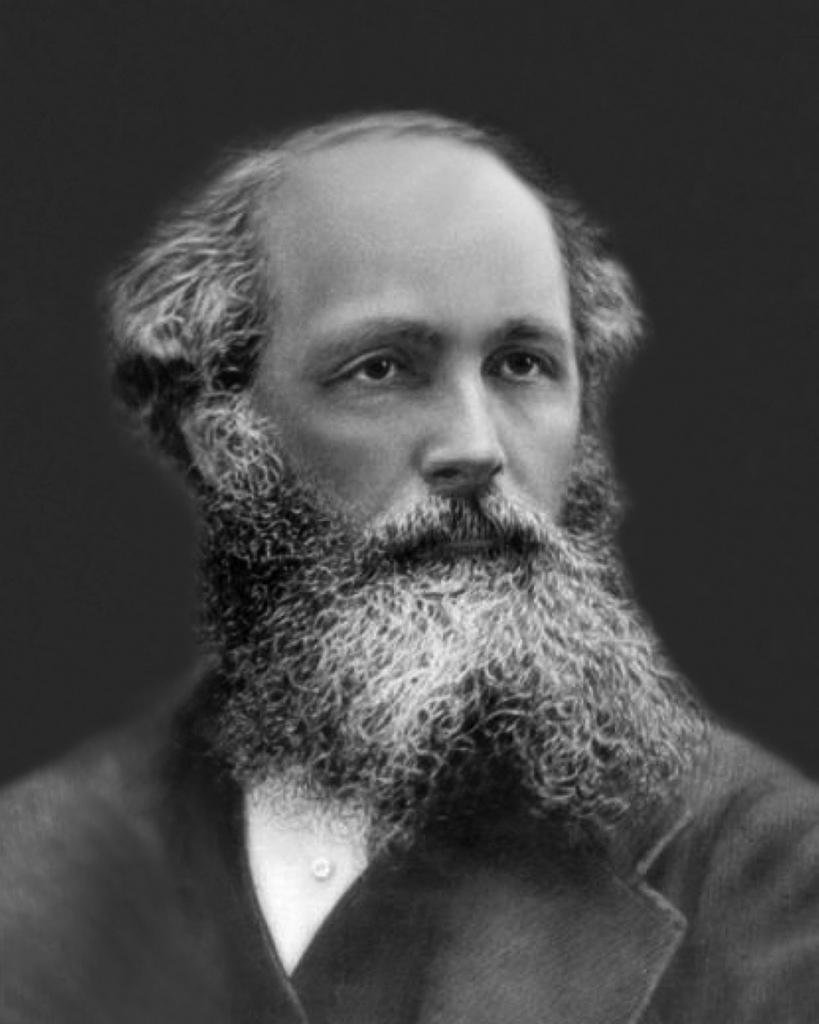
\includegraphics[width=0.4\textwidth]{figures/James-Clerk-Maxwell.jpg}
  %}{A picture of the Scottish physicist and mathematician James Clerk Maxwell from Wikimedia commons.}
    \caption{A picture of the Scottish physicist and mathematician from \href{https://upload.wikimedia.org/wikipedia/commons/b/b0/James-Clerk-Maxwell-1831-1879.jpg}{Wikimedia commons}.}
\end{figure}

If this confuses you then you are not alone. In the 1800's the Scottish Physicist James Clerk Maxwell had given a mathematical description of electricity and magnetism that unified them into the theory of \textbf{electromagnetism}. A consequence of this theory is that there are waves in the electromagnetic field, with light being an example of an electromagnetic wave. The theory also tells us that light always travels at the same speed, known as the speed of light $c=3\times 10^{8}\text{m/s}$.\\

Usually when we have waves they are travelling in a given medium. For example, water waves require water to move through, while sound waves are really pressure waves in the air or another substance.  This meant that many physicists expected there to be a medium, referred to as the \textbf{luminiferous aether} that light was a wave in. However, a range of experiments carried out by the American Physicists Michelson and Morley, showed that there was no such medium. This meant that an alternative explanation was needed for why light always travelled at the same speed regardless of how fast the object emitting light is travelling.\\

\begin{figure}[ht]
    \centering
    %\pdftooltip{
    \ThisAltText{ A picture of Albert Einstein from Wikimedia commons.}
    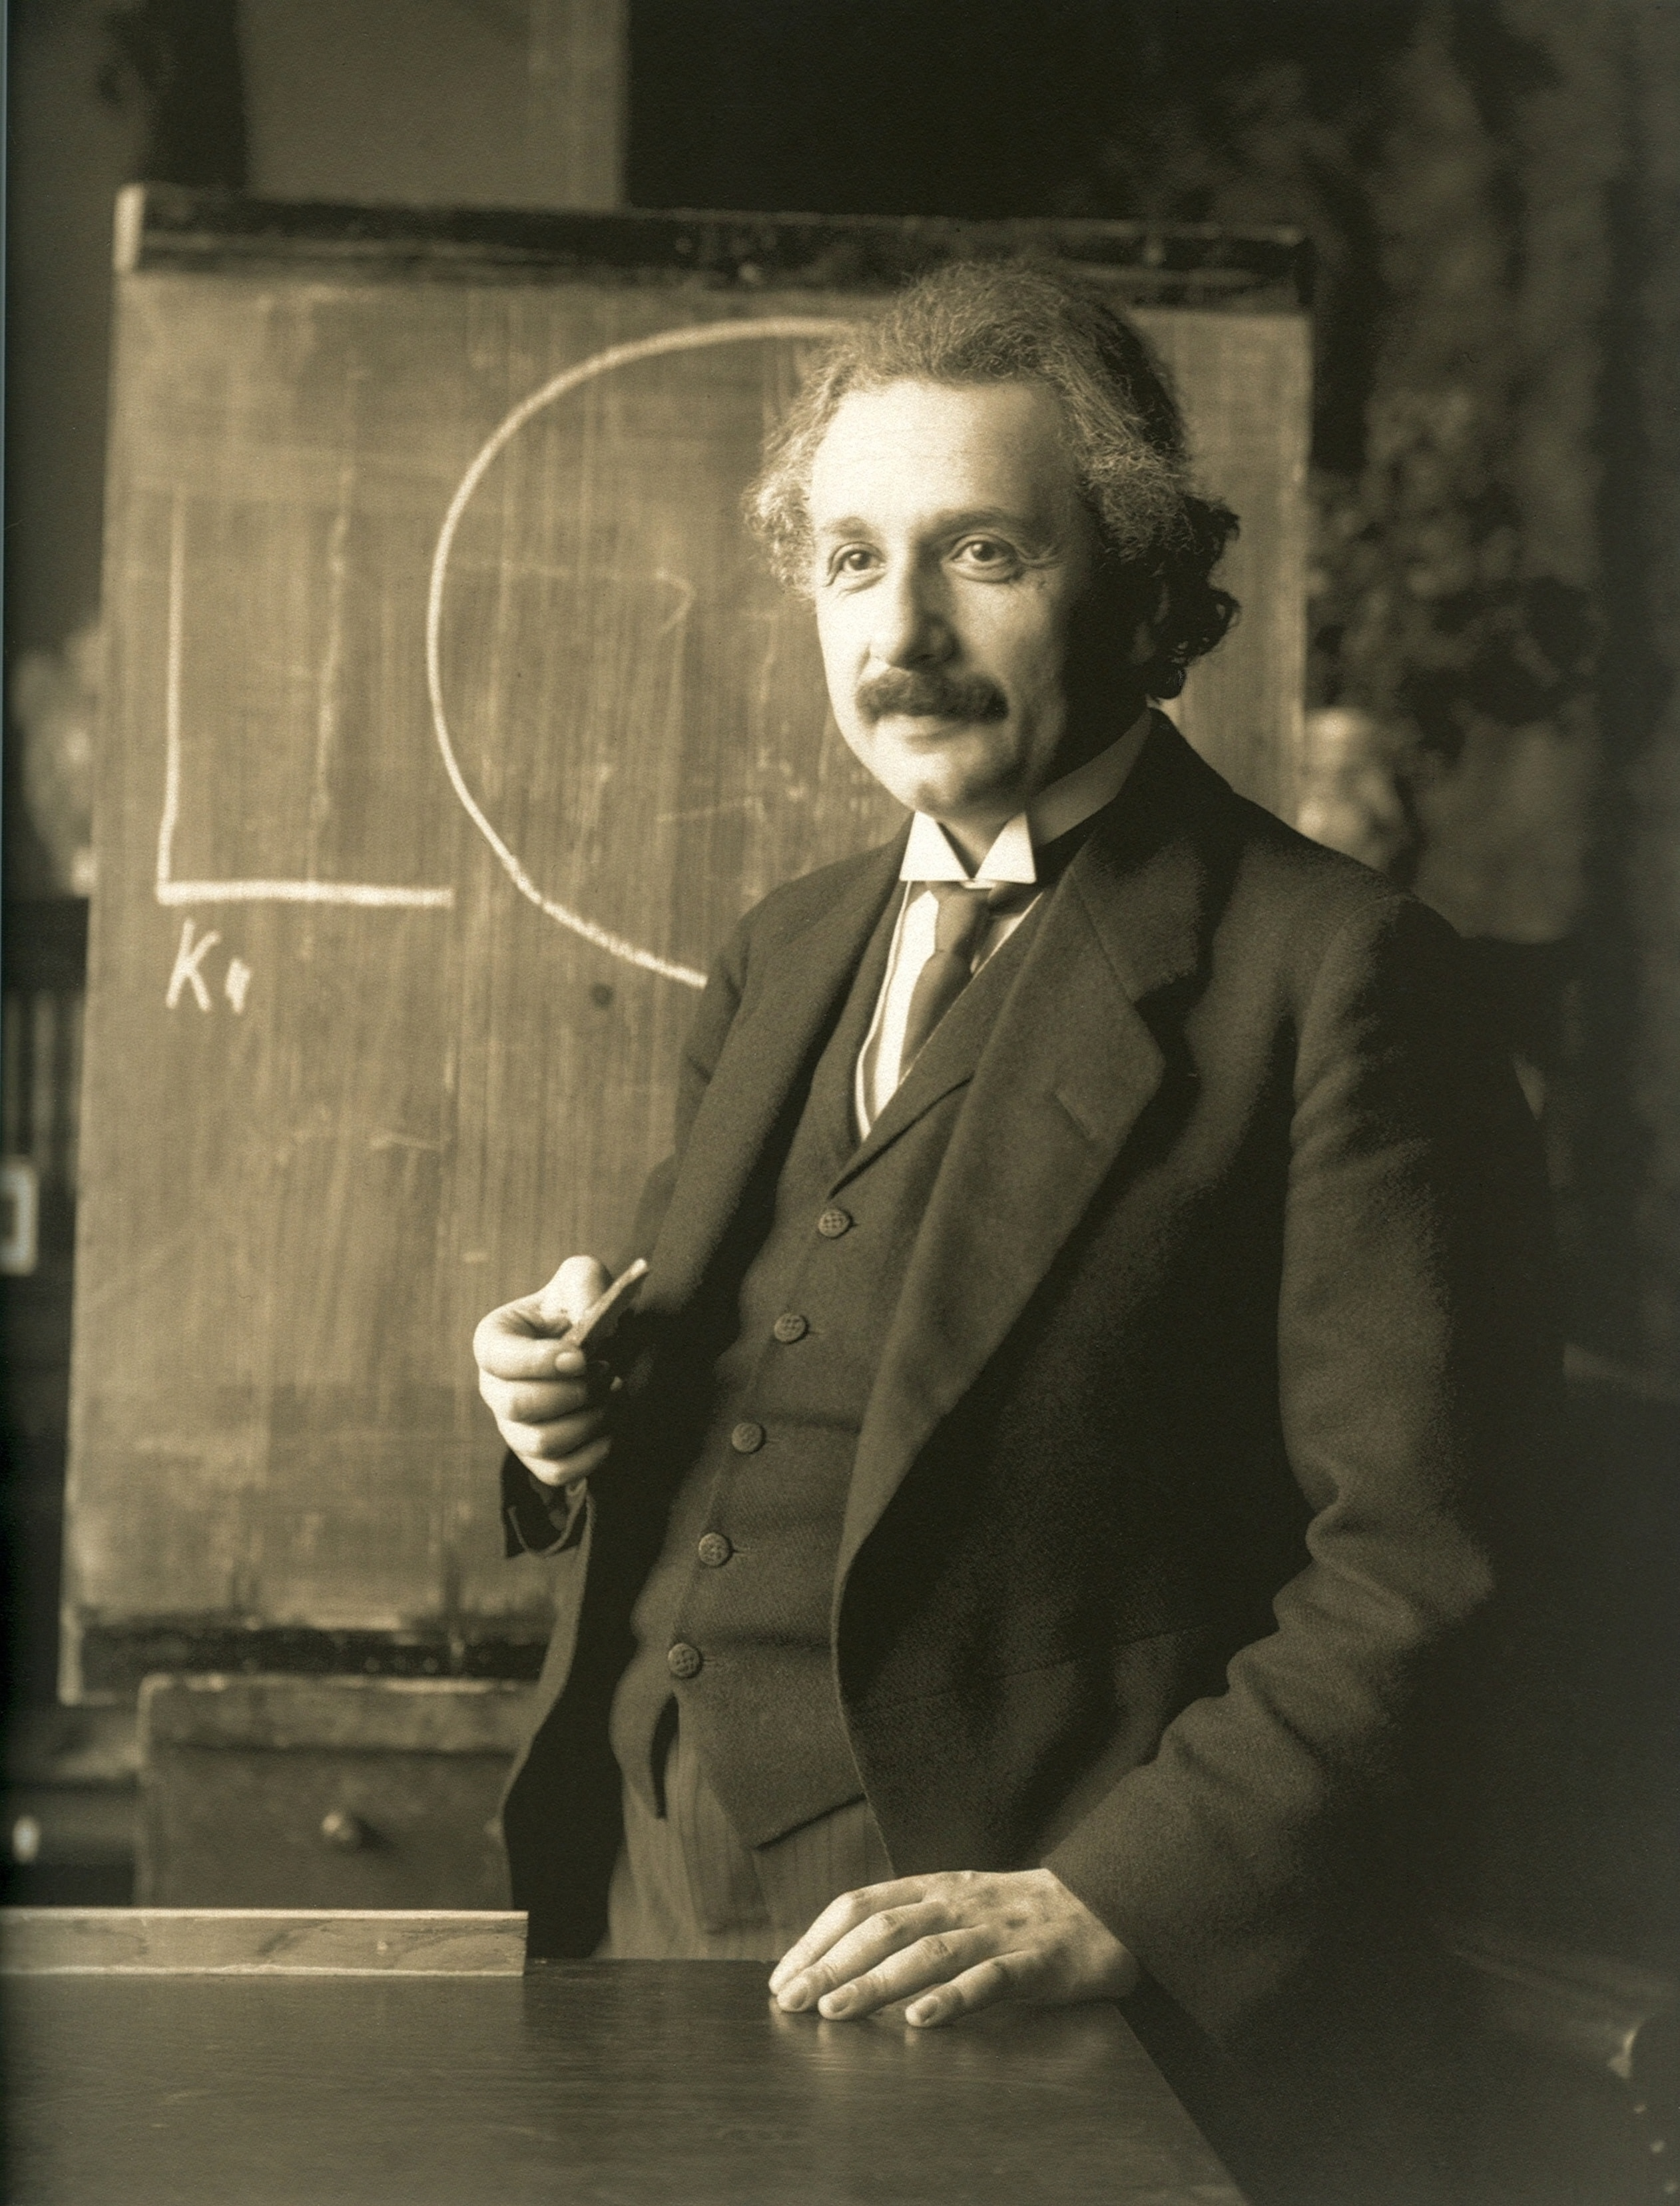
\includegraphics[width=0.4\textwidth]{figures/Einstein_1921_by_F_Schmutzer_-_restoration.jpg}
    %}{A picture of the German Physicist Albert Einstein from Wikimedia commons.}
    \caption{A picture of the German physicist Albert Einstein from \href{https://upload.wikimedia.org/wikipedia/commons/3/3e/Einstein_1921_by_F_Schmutzer_-_restoration.jpg}{Wikimedia commons}.}
\end{figure}

The eventual explanation was Einstein's theories of relativity, both \textbf{special relativity} and \textbf{general relatvity}.  Special relativity is based on two postulates:
\begin{itemize}
\setlength{\itemsep}{-5pt}
    \item[First:] The laws of physics are the same in all inertial frames.
    \item[Second:] The speed of light in vacuum is the same in all inertial frames.
\end{itemize}  

The second postulate implies that nothing can travel faster than the speed of light in vacuum $c=3\times 10^{8}\text{m/s}$. An important phrase in the postulates is \textbf{inertial frame}, this means that whoever is making the measurements is not accelerating. The word frame in the above postulates may seem confusing but it is just away of referring to a set of coordinate axes that move with an observer. So far in the module we have treated the coordinates $x,y,z$ and the time $t$ as absolute quantities that everyone performing measurements agrees on. However, a consequence of relativity is that this is not true, and the measurements that you make depend on how fast you are travelling.\\

This means that the Newtonian mechanics we studied throughout this module breaks down at high speeds. Do not despair about this, it does not mean that you should just bin everything that you have learnt so far. Everything that you have learnt is still valid, as long as you are not interested in very fast or massive objects. We will make this more precise shortly.\\

Consider a person moving with speed $v$ in the $x$ direction. \cref{fig: moving frames} shows the difference between the coordinates that our moving observer would use, and the coordinates that a stationary observer would use. By inspection of the figure we see that since the observer is only moving in the $x$-direction anything measured in $y$ and $z$ remains the same, this means that $y'=y,\,z'=z$.\\

\begin{figure}[ht]
    \centering
    \ThisAltText{ The Galilean relativity relationship between moving frames.}
    %\pdftooltip{
    \begin{tikzpicture}
\draw[black, ultra thick,->] (0,0) --(4,0) node[anchor=west]{$x$ axis};
\draw[black, ultra thick,->] (0,0) --(2,2) node[anchor=west]{$y$ axis};
\draw[black, ultra thick,->] (0,0) --(0,4) node[anchor=south]{$z$ axis};
\draw[black, ultra thick,->] (8,0) --(12,0) node[anchor=west]{$x'$ axis};
\draw[black, ultra thick,->] (8,0) --(10,2) node[anchor=west]{$y'$ axis};
\draw[black, ultra thick,->] (8,0) --(8,4) node[anchor=south]{$z'$ axis};
\draw[blue, ultra thick, ->] (8,0) --(10,0) node[anchor=north]{$v$};
\end{tikzpicture}
%}{Comparison of a fixed frame with a frame moving at speed $v$ in the $x$-direction.}
    \caption{Comparison of a fixed frame with a frame moving at speed $v$ in the $x$-direction.}
    \label{fig: moving frames}
\end{figure} 

At slow speeds this is actually known as \textbf{Galilean relativity}, and we have that $x'=x-vt$. That is to convert from what is measured by the stationary observer to the moving observer we have to take account of how far the moving observer has travelled by the time they make the measurement. This sort of relativity does not pose any problems for what we have learnt in this module, the novelty comes if the observer is moving close to the speed of light. Then the relationship between $x$ and $x'$ is given by a different formula known as a \text{Lorentz transform}:
\begin{equation}
x'=\frac{x-vt}{\sqrt{1-\frac{v^{2}}{c^{2}}}}.
\label{eq: length contraction}
\end{equation}
More surprisingly, if the moving observer is carrying a clock, this will measure time at a different rate than a clock held by a stationary observer. This is something new and does not happen for Galilean relativity. If the clock held by a stationary observer shows a time $t$, then if they look at the clock held by the moving observer it will show a time
\begin{equation}
t'=\frac{t-\frac{v}{c^{2}}x}{\sqrt{1-\frac{v^{2}}{c^{2}}}}.
\label{eq: time dilation}
\end{equation}

The new part of these expressions is so important that it is called the \textbf{Lorentz factor}, or sometimes the gamma factor, and is given the symbol
\begin{equation}
\upgamma=\frac{1}{\sqrt{1-\frac{v^{2}}{c^{2}}}},
\end{equation}
some books will also call the ratio of the speed $v$ to the speed of light $\upbeta=v/c$.\\

An immediate consequence of these expressions is that a stationary observer will see the moving observer shrink\footnote{This is known as \textbf{length contraction}}, in the direction they are moving in, and will see the moving clock speeding up\footnote{This is known as \textbf{time dilation}}. The second phenomena is usually phrased from the point of view of the moving observer who will see the stationary observers clock moving more slowly than their own.\\

With length contraction, we can phrase it in a different way by. The length is the difference between two positions $x_{1}'$ and $x_{2}'$, we call the length measured in the moving frame $L_{0}=x_{2}'-x_{1}'$ and the length measured in the stationary frame $L$.
\begin{align*}
L_{0}&=x_{2}'-x_{1}'\\
	&=\frac{x_{2}-vt}{\sqrt{1-\frac{v^{2}}{c^{2}}}}-\frac{x_{1}-vt}{\sqrt{1-\frac{v^{2}}{c^{2}}}}\\
	&=\frac{x_{2}-x_{1}}{\sqrt{1-\frac{v^{2}}{c^{2}}}}\\
	&=\upgamma L.
\end{align*}

\paragraph{Example 9.1:} The Voyager spacecraft has a length of $4\text{m}$ and is moving at $12 260\text{m/s}$. How long does it appear to an observer on Earth?\\

We are given the length in the moving frame $L_{0}=4\text{m}$ so we just need to compute 
\begin{equation*}
\upgamma=\frac{1}{\sqrt{1-\frac{v^{2}}{c^{2}}}}=\frac{1}{\sqrt{1-\frac{(17260)^{2}}{(3\times10^{8})^{2}}}}=\frac{1}{0.9999999834496}=1.000000001655042.
\end{equation*}
We then know that $L_{0}=L\upgamma$ or $L=L_{0}/\upgamma$ so
\begin{equation*}
L=\frac{L_{0}}{\upgamma}=4\times0.9999999834496=3.99999999337981\text{m}.
\end{equation*}

This is a very small difference, and shows you just how fast an object has to be travelling for there to be an observable difference in the length. To find when the change in length is considerable we can compute the gamma factor for $v=c/2$,
\begin{equation*}
\upgamma=\frac{1}{\sqrt{1-\frac{1}{4}}}=\frac{2}{\sqrt{3}}=1.1547,
\end{equation*}
and for $v=9c/10$,
\begin{equation*}
\upgamma=\frac{1}{\sqrt{1-\frac{81}{100}}}=\frac{10}{\sqrt{19}}=2.29.
\end{equation*}
What do these mean for the observed length of voyager from Earth:
\begin{align*}
\text{for } v=c/2 \quad L&=\frac{L_{0}}{\upgamma}=\frac{4}{1.1547}=3.46\text{m},\\
\text{for } v=9c/10 \quad L&=\frac{L_{0}}{\upgamma}=\frac{4}{2.29}=1.74\text{m},
\end{align*}
so at both of these speeds we see a much more significant change in the length.\\

So far we have just been sketching out what happens when objects are moving very quickly. Another consequence of special relativity is the relationship of mass and energy through,
\begin{equation}
E=mc^{2}.
\end{equation}
This is another of Einstein's famous results, and says that every object has an intrinsic energy associated with its mass. This is a very important relationship if you are interested in nuclear energy as it is this intrinsic mass energy which is accessed via fission and fusion. \\

There is also general relativity which is Einstein's theory of gravitation, but this is a much more complicated story and we will not say anything about it here.

\section{Quantum Quandaries}
Now we turn from the very fast to the very small.  For an introduction to the wonderful world of quantum physics I recommend the 43rd and 44th videos from the crash course physics playlist available \href{https://www.youtube.com/playlist?list=PL8dPuuaLjXtN0ge7yDk_UA0ldZJdhwkoV}{here}.  The book \textbf{Quantum Physics: A Beginner's Guide } by Rae, \citep{rae2005quantum}, is available in the library and is a good jumping off point if you want to learn more about the counter intuitive world of quantum physics.\\

Quantum physics deals with the very smallest objects. These are fundamental particles like the electron, which we met as the charge carrier responsible for electric current. In most of this module we have thought in terms of balls rolling down slopes, juggling balls moving along a parabola, springs pendulums oscillating backwards and forwards. You may also have seen artists impressions of atoms where they are represented as being mini solar systems with the electrons orbiting around a central positively charged nucleus.  However, this is not really what is going on.\\

At the smallest scale, particles are waves and waves are particles!\\

You are probably asking ``what does this mean?'' The answer is that what you observe when you look at something depends on how you look at it. \\

The most famous example of this is what is known as the double slit experiment. If we imagine having two screens set up, one with two slits cut in it so that can pass through the holes in the first screen and then hit the second screen. This is shown for classical particles and waves in \cref{fig: double slit particle,fig: double slit waves} respectively. For classical particles they either pass through one slit or the other and will strike the second screen in line with the slits. This would result in the pattern shown in \cref{fig: double slit particle}.\\

\begin{figure}[ht]
    \centering
    \ThisAltText{ A picture of the double slit experiment for particles taken from Wikimedia commons.}
   % \pdftooltip{
   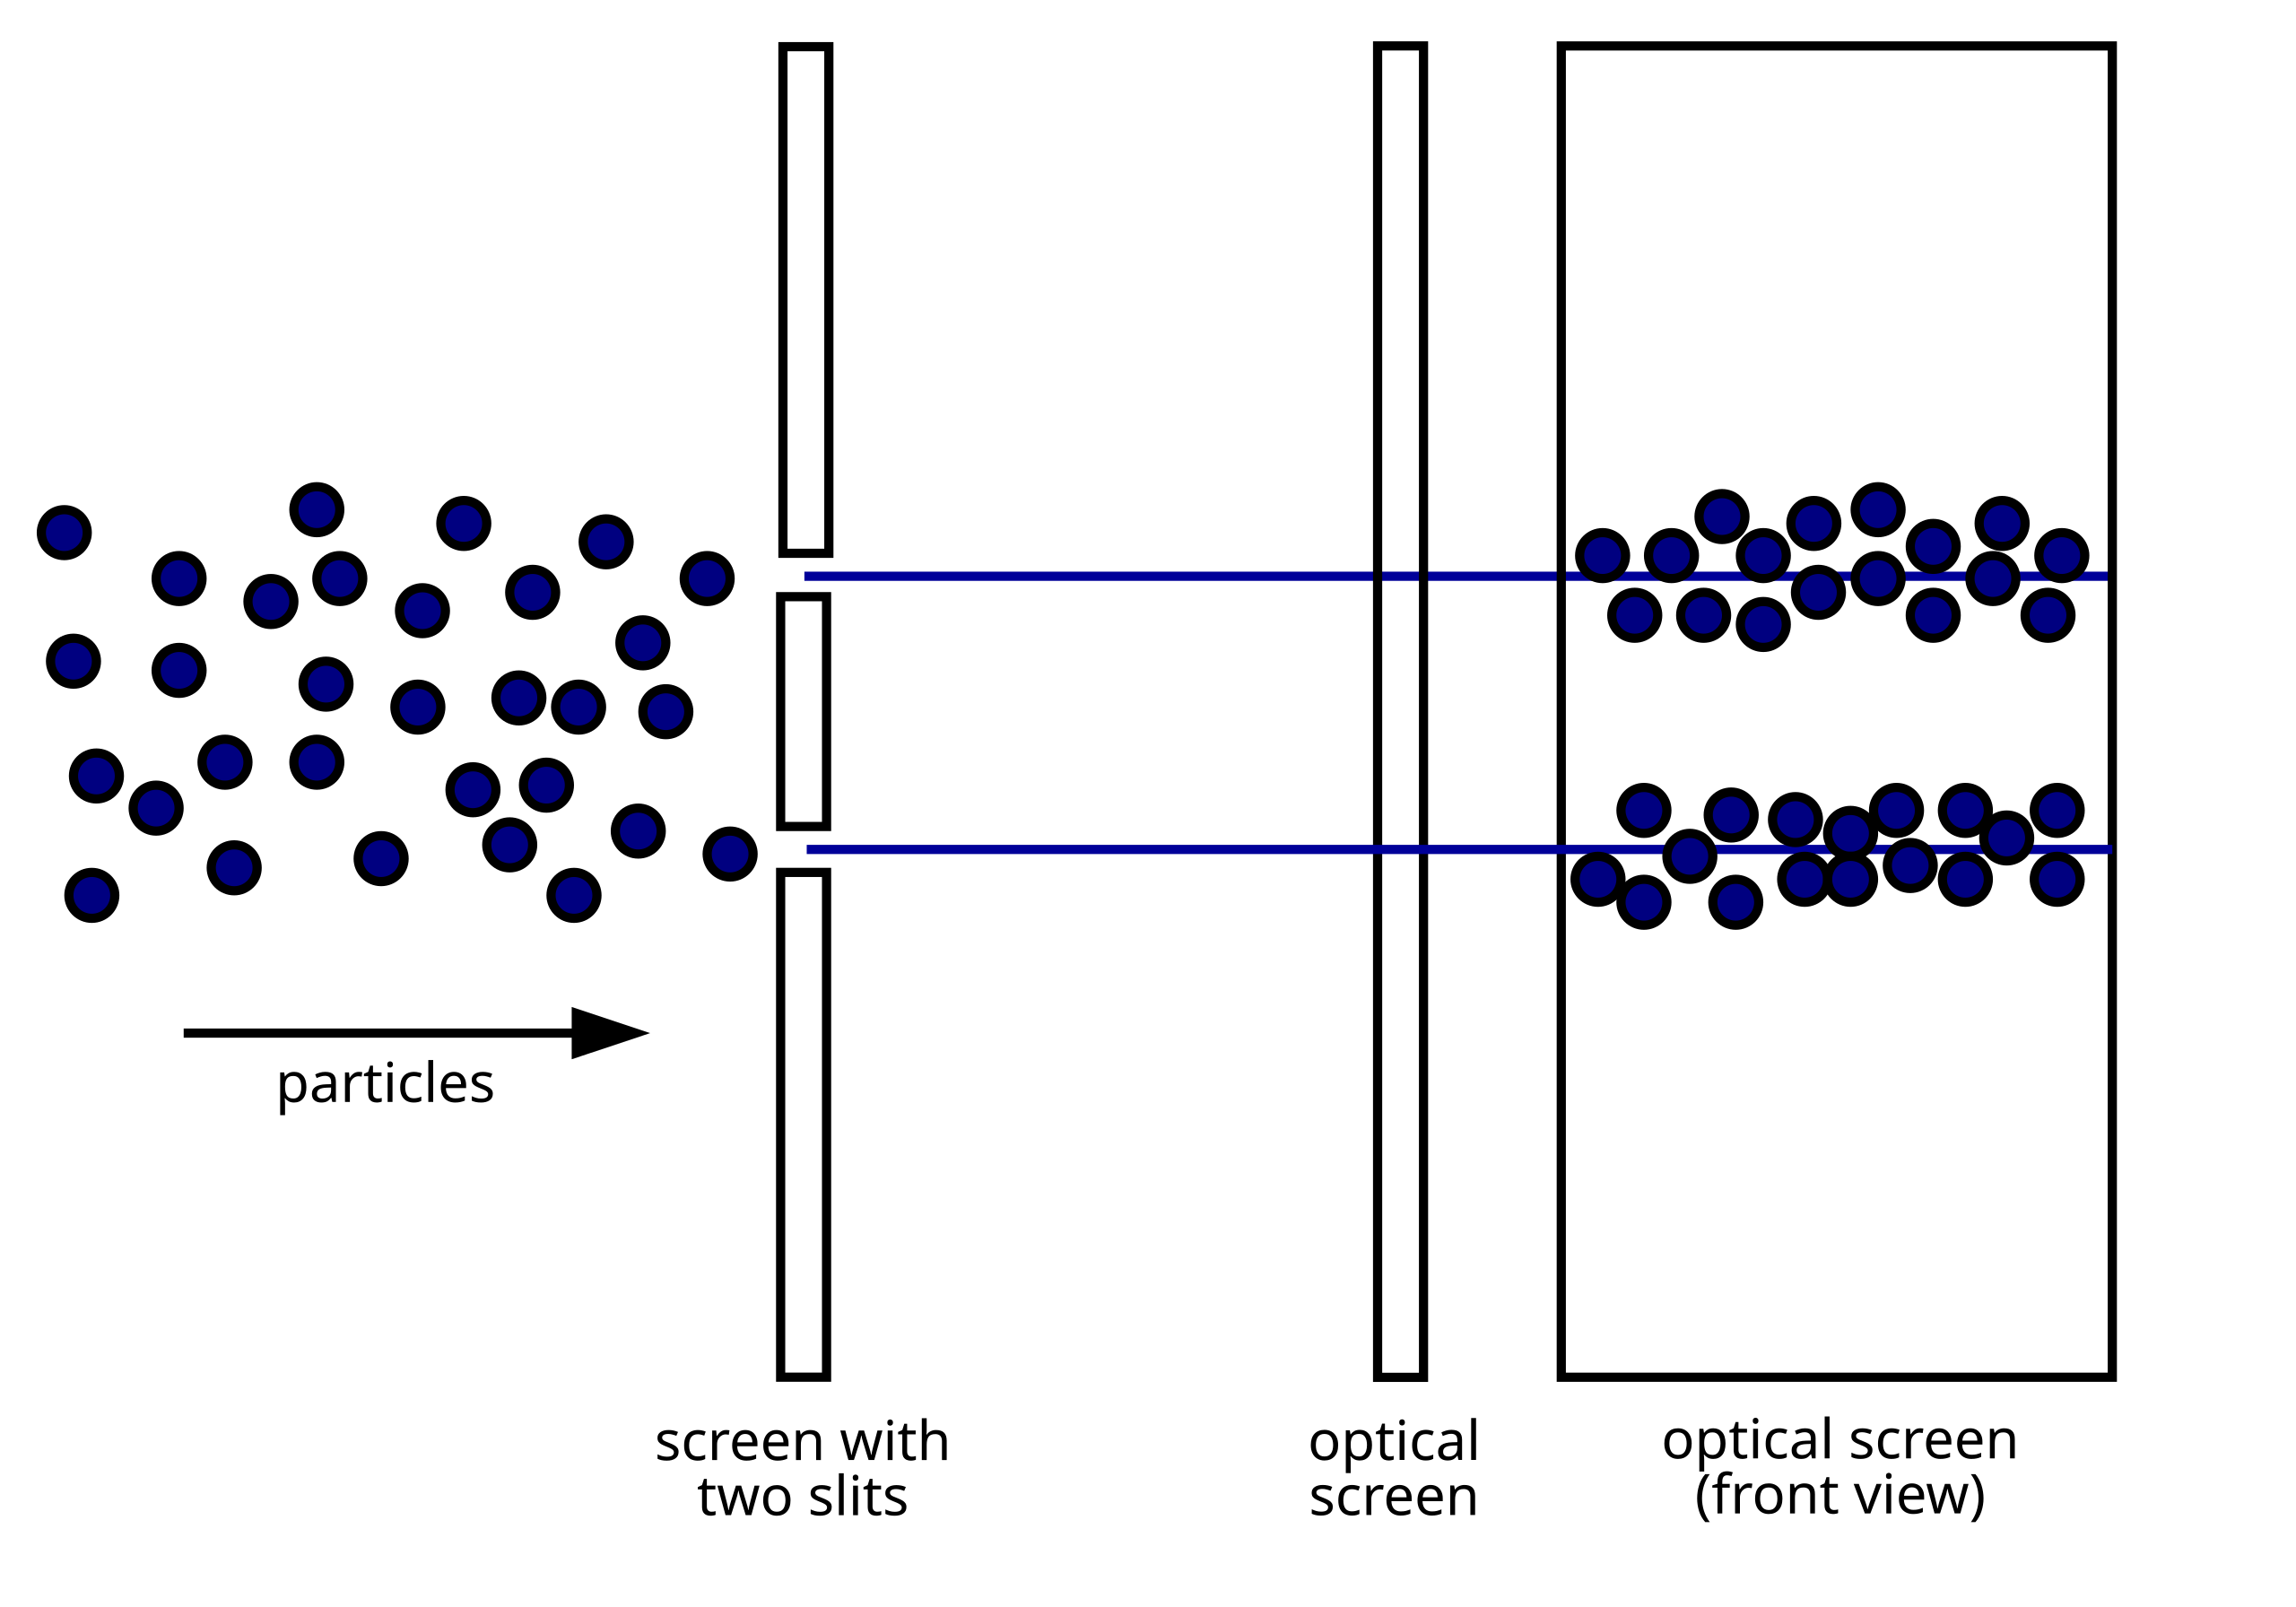
\includegraphics[width=0.5\textwidth]{figures/Two-Slit_Experiment_Particles.png}
   %}{A picture of the double slit experiment for particles from Wikimedia commons.}
    \caption{A picture of the double slit experiment for particles from \href{https://commons.wikimedia.org/wiki/File:Two-Slit_Experiment_Particles.svg}{Wikimedia commons}.}
    \label{fig: double slit particle}
\end{figure}

When a wave passes through a slit it \textbf{diffracts}\footnote{This means that it bends as it passes through the aperture. Diffraction is one of the hallmark behaviour of waves.}. When there are two slits the wave passes through both and diffracts so we have two sets of wavefronts one emerging from each of the slits. These wavefronts then \textbf{interfere}\footnote{Interference is another hallmark behaviour of waves. It means that when two waves overlap they add together so if a peak lies on top of a peak this leads to a wave with an even bigger peak, if a trough lies on top of a trough it leads to an even deeper trough, both called constructive interference. While if a peak lies on top of a trough they cancel out, called destructive interference.. } with each other, and we see an interference pattern on the second screen. This means that there is an intensity peak in the middle of the screen, with a sequence of peaks of decreasing brightness spread out on the screen. This is shown in \cref{fig: double slit waves}.\\

\begin{figure}[ht]
    \centering
    \ThisAltText{ A picture of the double slit experiment for waves taken from Wikimedia commons.}
    %\pdftooltip{
    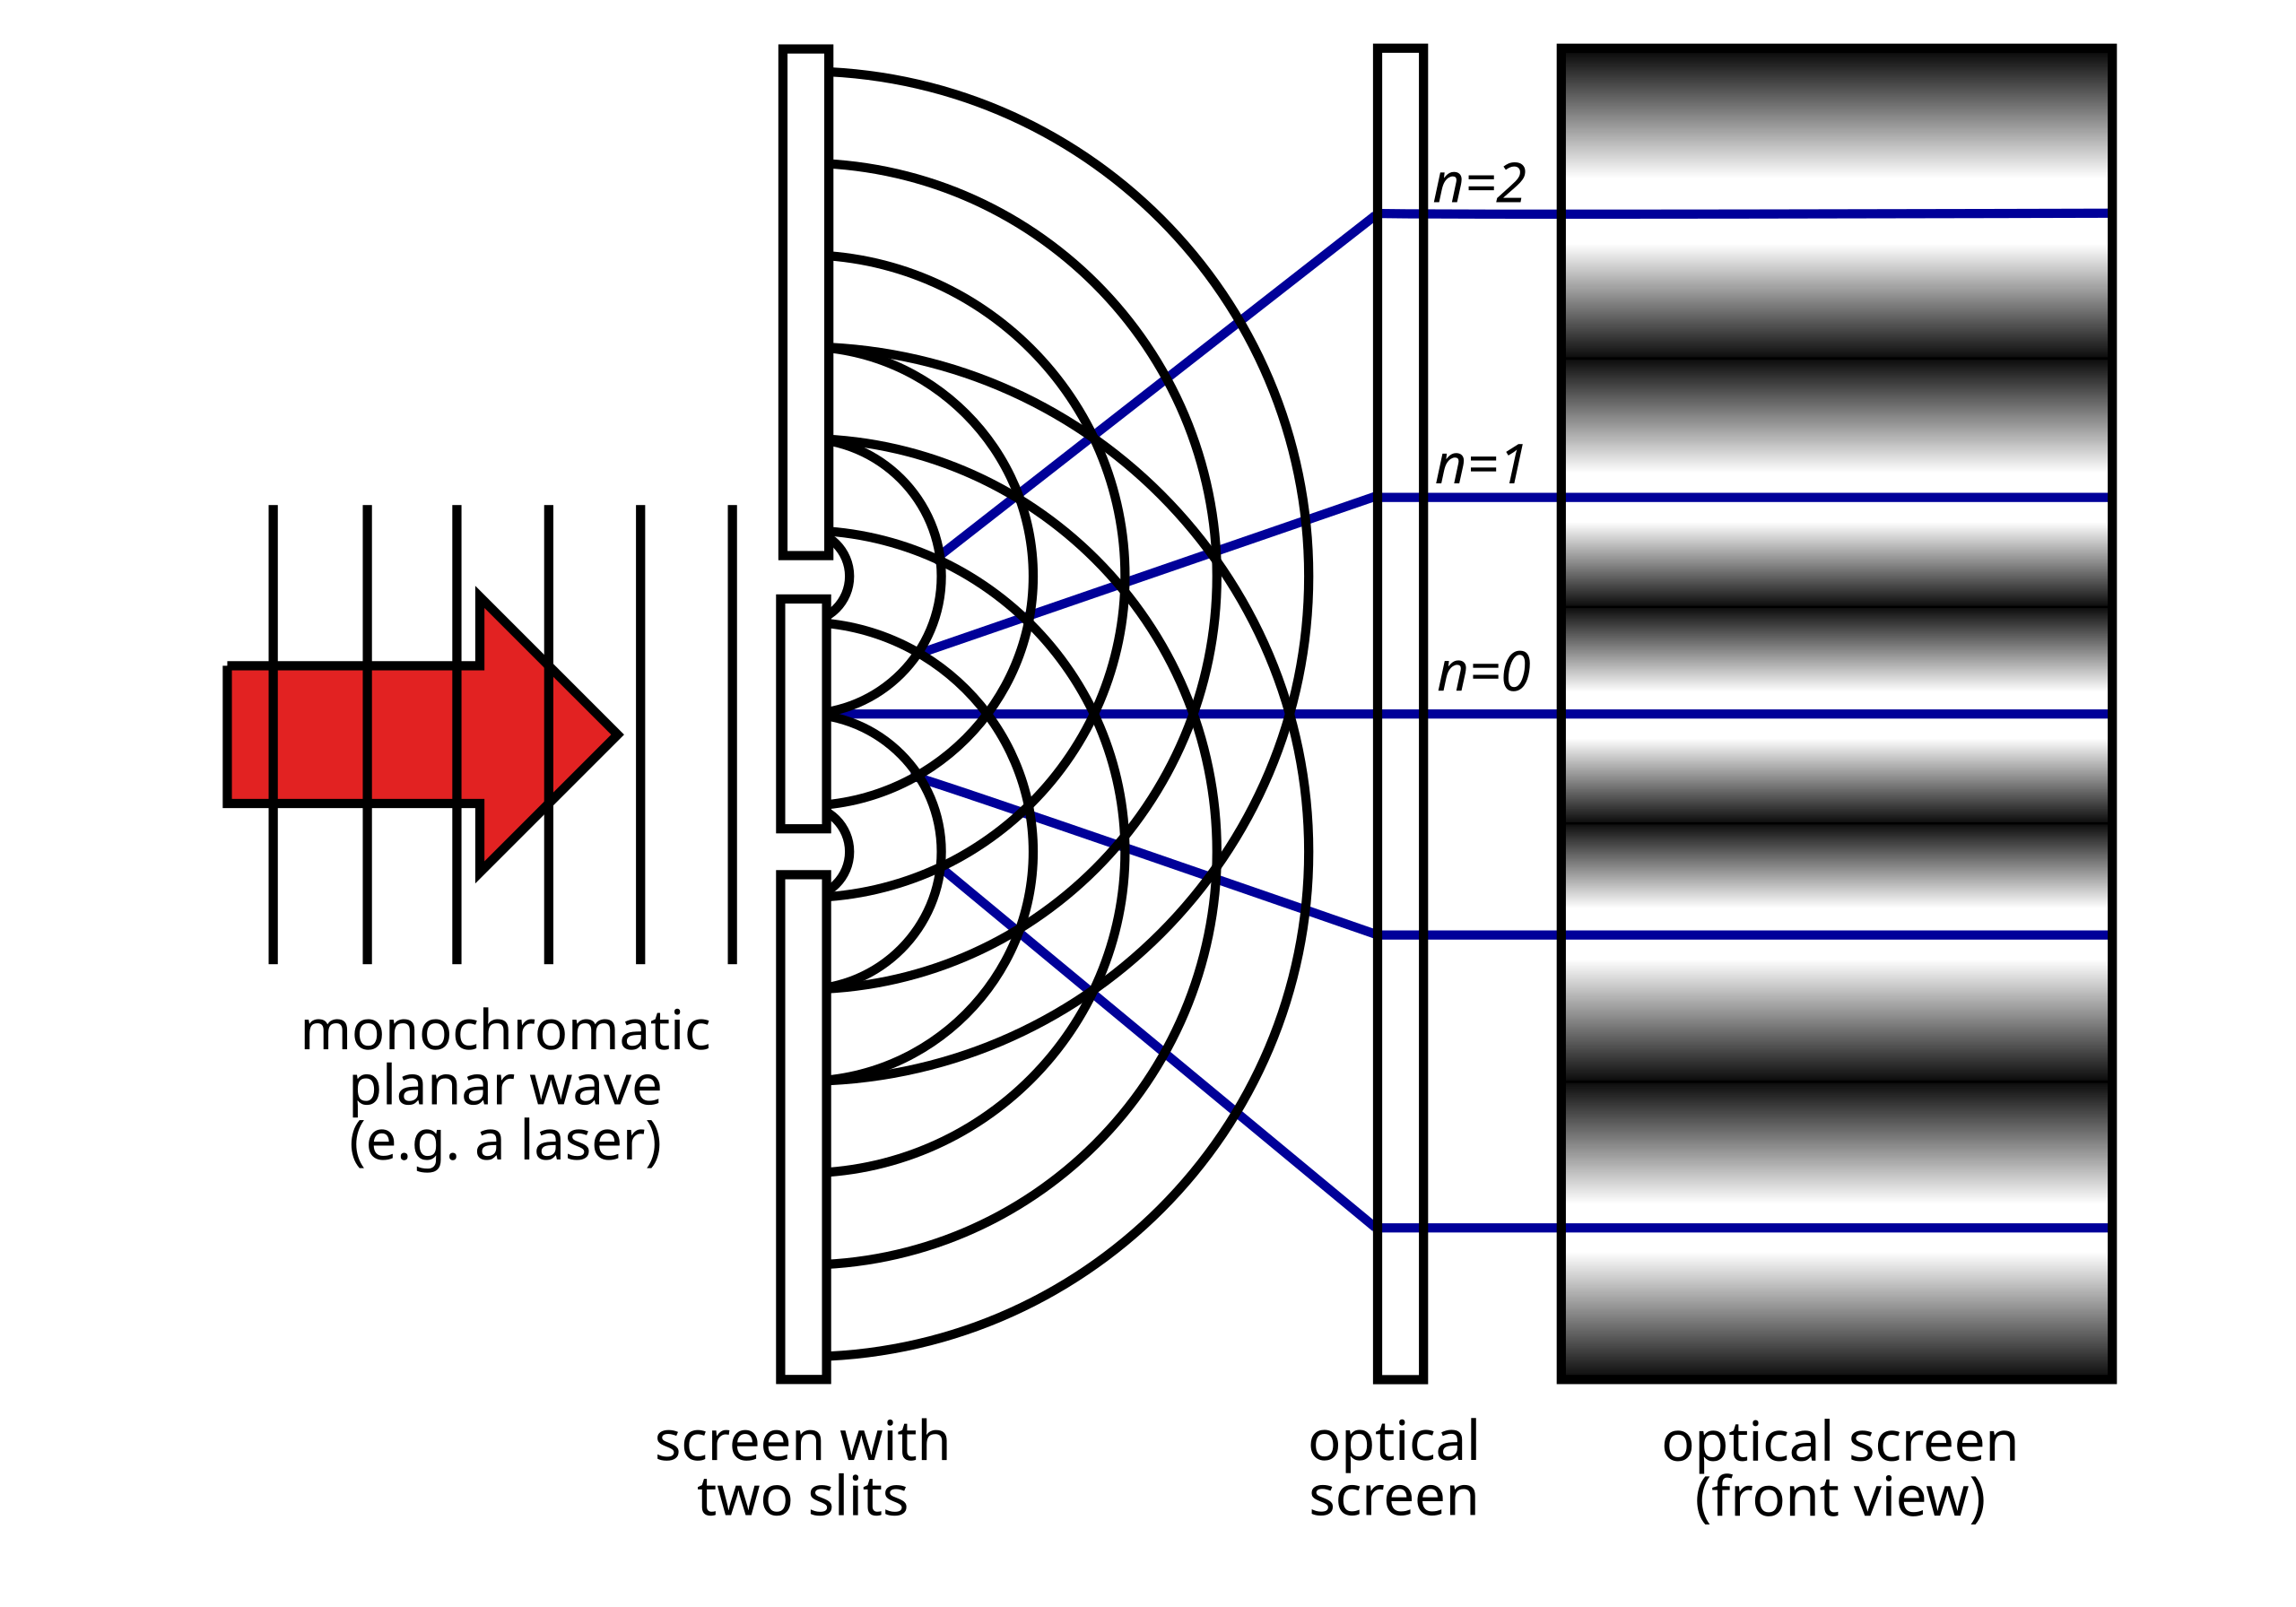
\includegraphics[width=0.5\textwidth]{figures/Two-Slit_Experiment_Light.png}
    %}{A picture of the double slit experiment for waves from Wikimedia commons.}
    \caption{A picture of the double slit experiment for waves from \href{https://commons.wikimedia.org/wiki/File:Two-Slit_Experiment_Light.svg}{Wikimedia commons}.}
    \label{fig: double slit waves}
\end{figure}

The double slit experiment was first performed by Thomas Young in 1801 and was taken as a demonstration that light behaved like a wave, as Young observed the wave-like interference pattern. However, at the turn of the twentieth century both Max Planck and Albert Einstein gave theoretical evidence that light should be treated as a particle in certain circumstances. Planck did this to explain \textbf{black-body radiation}, the radiation emitted by a body in thermal equilibrium with its environment. While Einstein presented a solution to the \textbf{photoelectric effect}, the emission of electrons from a material when light with a specific wavelength is shone on the material. Both of these explanations rely on thinking of light as being made up of \textbf{quanta}, or lumps, of energy known as \textbf{photons}. This is the first evidence of what is known as \textbf{wave-particle duality}, the fact that some objects can behave like a wave or a particle depending how you look at them. \\

In the 1920's the French Physicists Louis de Broglie took this a step further and proposed that objects like electrons and protons that were thought of as being particles, could behave like waves in certain circumstances. This was then tested by carrying out a double slit experiment for electrons, see \cref{fig: double slit electrons} for a schematic of this.  It turns out that even if you slow this down so much that only one electron at a time is being emitted, you still see an interference pattern so somehow the electron is interfering with itself.\\

It is natural to ask if we can just watch one of the slits and see does the electron pass through or not. If we do this then we will either see an electron pass through or not, but now on the second screen we observe the particle like picture from \cref{fig: double slit particle}. The surprising results is that if you try to observe a particle like property of an electron, or any other sub atomic particle, you get a particle like answer, while if you try to observe a wave like property you get a wave like answer.\\

\begin{figure}[ht]
    \centering
    %\pdftooltip{
    \ThisAltText{ A picture of the double slit experiment for quantum objects taken from Wikimedia commons.}
    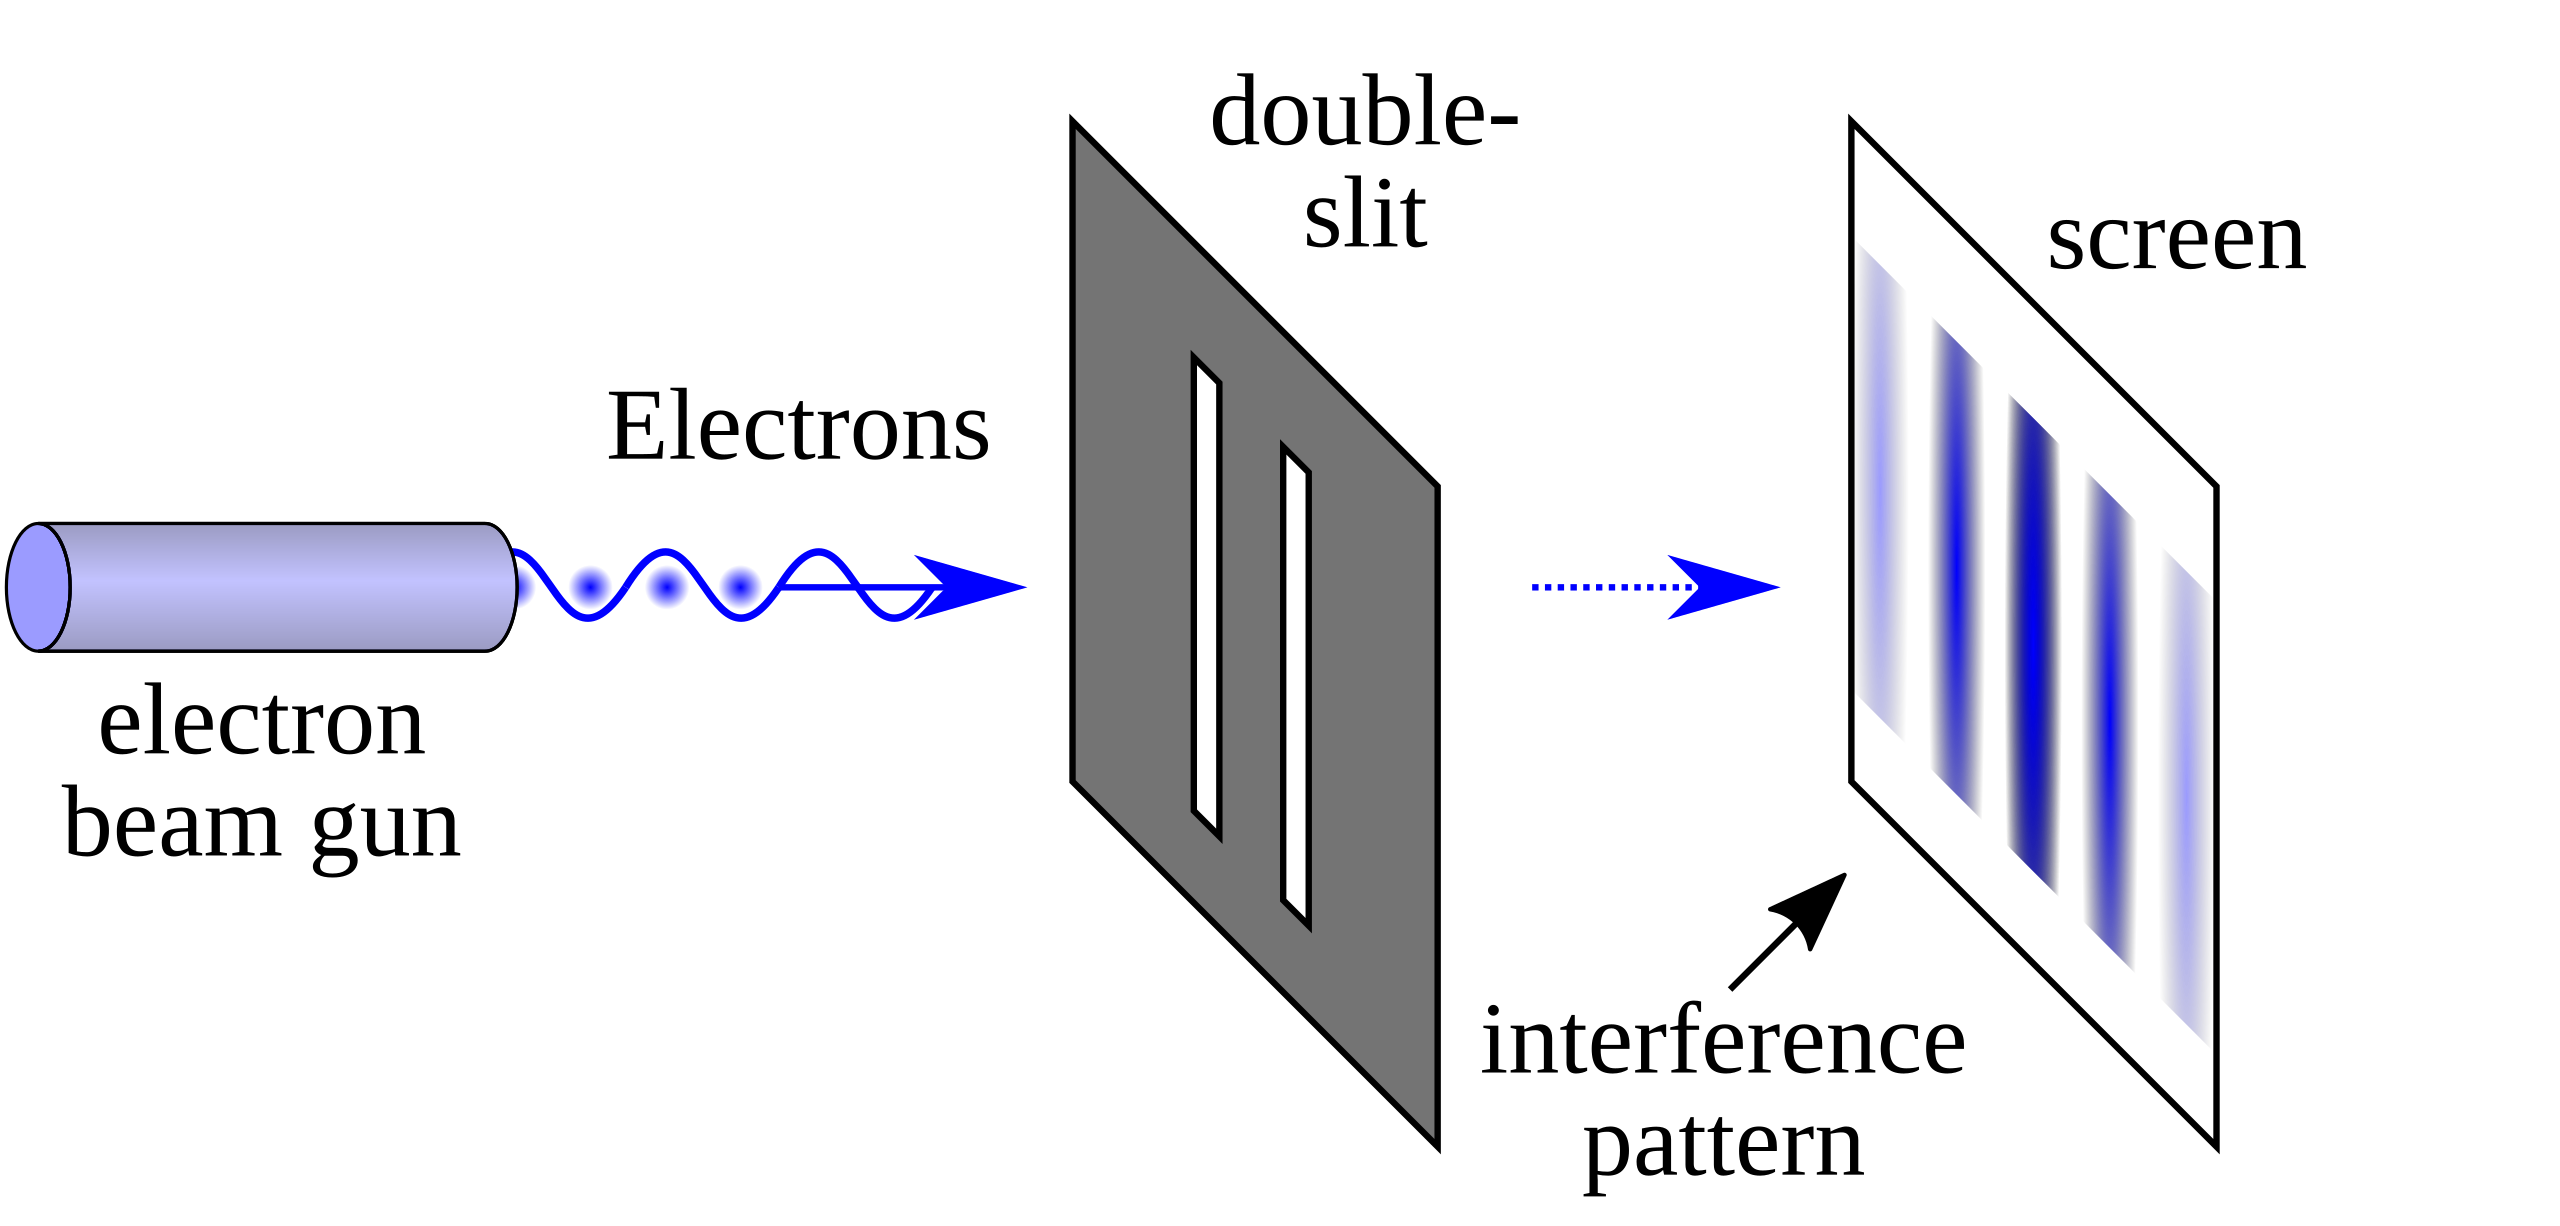
\includegraphics[width=0.5\textwidth]{figures/double_slit_electrons.png}
    %}{A picture of the double slit experiment for electrons from Wikimedia commons.}
    \caption{A picture of the double slit experiment for electrons from \href{https://commons.wikimedia.org/wiki/File:Double-slit.svg}{Wikimedia commons}.}
    \label{fig: double slit electrons}
\end{figure}

If this sounds completely crazy to you then you are not alone. It is an incredibly counter intuitive observation, in the everyday world a football does not swap between being a solid ball and a wave depending on how I observe it. However on the quantum scale this really does happen. Discoveries like this lead the physicist Richard Feynman to say ``Nobody understands quantum mechanics'', and leads on to a school of thought called ``shut up and calculate''. This point of view is essentially that you should forget about trying to draw pictures of what is going on  and trying to describe complete trajectories. Instead focus on what you can observe, and let the mathematics guide you. 

%\begin{warpprint} % For print output ...
%\cleardoublepage % ... a common method to place index entry into TOC.
%\phantomsection
%\addcontentsline{toc}{chapter}{\indexname}
%\end{warpprint}
%\ForceHTMLPage % HTML index will be on its own page.
%\ForceHTMLTOC % HTML index will have its own toc entry.
%\printindex

%%%%%%%%%%%%%%%%%%%%%%%%%%%%%%%%%%%%%%%%%%%%%%%%%%%%%%%%%%%%%%%%%%%%%%%

\chapter{Mathematical Basics}
\section{Background and References}
Physics is by its very nature a mathematical subject and it gets progressively more mathematical the further you take your studies of it. This means that to understand the material in the module and to be able to solve the tutorial problems, you need to have a experience with a variety of mathematical techniques such as:
\begin{itemize}
\setlength{\itemsep}{-5pt}
    \item solving linear equation,
    \item solving quadratic equations
    \item using trigonometry,
    \item using scientific notation and understanding 
    \item knowing what a vector and being able to calculate its magnitude and direction.
\end{itemize}

You will meet many of these topics in STM0001 Applied Mathematics which you are taking at the same time as this module, and I am aiming to briefly introduce any new mathematical topics when we need them. However, I also want to link to some extra resources where you can brush up on your maths beforehand.\\


A great resource is the website \href{https://tutorial.math.lamar.edu/}{Pauls Online Math Notes}. The website contains notes for a variety of mathematics courses including algebra and calculus. The most useful material to complement this Physics module are the Algebra and trigonometry review \href{https://tutorial.math.lamar.edu/Extras/AlgebraTrigReview/AlgebraTrigIntro.aspx}{linked here} and the preliminaries section of the algebra notes, \href{https://tutorial.math.lamar.edu/Classes/Alg/Preliminaries.aspx}{linked here}.\\

As the module goes on I may add more maths resources or add some examples. In the first few weeks of tutorial problems there will be some maths problems for extra practice.\\

The essential maths skills needed for studying physics at this level are nicely summarised in \citep{garrett2015essential}. It is worth having a look at this book if you want to revise the maths background.

\section{Trigonometry Primer}
Since trigonometry comes up a lot in this course a review of the basics is included here. If you are not familiar with it you can either check out the links suggested above or ask me to provide more background information.\\

For our purposes we will only need trigonometry for right angled triangles. \textbf{Trigonometry} is an area of mathematics related to the study of triangles and provides a way to compute the lengths and angles in a triangle provided that you now some of them already.

\begin{figure}[ht]
    \centering
    %\pdftooltip{
    \ThisAltText{ A right angle triangle showing the trigonometric relationships between side lengths and angles.}
    \begin{tikzpicture}[scale=2]
  \coordinate [label=left:$\uptheta$] (C) at (-1.5cm,-1.cm);
  \coordinate (A) at (1.5cm,-1.0cm);
  \coordinate [label=above:$\upphi$] (B) at (1.5cm,1.0cm);
  \draw (C) -- node[above] {$a$} (B) -- node[right] {$c$} (A) -- node[below] {$b$} (C);
  \draw (1.25cm,-1.0cm) rectangle (1.5cm,-0.75cm);
  \tkzMarkAngle[size=1cm,color=blue](A,C,B)
  \tkzMarkAngle[size=1cm,color=blue](C,B,A)
\end{tikzpicture}
%}{A right angle triangle with all the angles and sides marked.}
    \caption{A right angle triangle with all the angles and sides marked.}
    \label{fig: Trig definitions}
\end{figure}

The typical mnemonic used to remember trigonometry is \textbf{SOH CAH TOA} which means Sine is opposite over hypotenuse
\begin{equation*}
\sin\uptheta=\frac{c}{a}, \qquad \sin\upphi =\frac{b}{a},
\end{equation*}
Cosine is adjacent divided by hypotenuse
\begin{equation*}
\cos\uptheta=\frac{b}{a}, \qquad \cos\upphi =\frac{c}{a},
\end{equation*}
and Tangent is opposite divided by adjacent
\begin{equation*}
\tan\uptheta=\frac{c}{b}, \qquad \sin\upphi =\frac{b}{c}.
\end{equation*}
There are associated inverse functions $\arcsin,\arccos,\arctan$ which convert ratios of sides into angles. All of these functions are available on your calculator. \\

It is important to be careful with which units you are using to express angles. It is likely that you will have come across degrees where going around a full circle is represented by an angle of $360^{\circ}$. However, it is often convenient to work with a different measure of angles called radians, in this case we take a full circle to be $2\uppi\text{rad}$ and express angles as a number between $0$ and $2\uppi$. In this module you can probably get away with always working in degrees, other than for some of the formulas quoted for the pendulum. However, if you go further with maths or physics you will find that radians as much more convenient to work with.

\section{Rearranging Equations}
A very important skill for solving physics problems is to be able to rearrange equations. This is sometimes referred to as changing the subject of an equation. Newcastle University have a webpage, available \href{https://www.mas.ncl.ac.uk/ask/numeracy-maths-statistics/core-mathematics/pure-maths/algebra/rearranging-equations.html}{here} that goes through some examples of how to rearrange equations. The webpage also has some self test questions that you can look at if you want more practice. Some of the details are reviewed here, along with examples for the specific equations that we have been using in this module.\\


In the equation
\begin{equation*}
x=5y+4z,
\end{equation*}
$x$ is called the subject, which is just a fancy way of saying that $x$ is expressed in terms of the other variables. When we talk about rearranging an equation, we mean that we change the subject of the equation from $x$ to another variable like $y$ and $z$. We do this by performing a variety of mathematical operations to both sides of the equation to swap some of the variables from one side to the other. \\

These operations can include: adding or subtracting a quantity from both sides, multiplying or dividing by a quantity, taking logarithms of or exponentiating both sides of the equation, raising both sides of the equation to any non-zero power.\\

Returning to the above equation $x=5y+4x$, we can rearrange it to make $z$ the subject. Again, this means that we will perform mathematical operations on both sides of the equation to put it in the form $z=\dots{}$ : 
\begin{align*}
x&=5y+4z, \quad \text{ first subtract $5y$ from both sides},\\
x-5y&=5y+4z-5y=4z, \quad \text{then divide both sides by 4},\\
\frac{x-5y}{4}&=\frac{4z}{4}=z.
\end{align*}
This gives us
\begin{equation*}
z=\frac{x-5y}{4},
\end{equation*}
with $z$ now the subject of the equation.\\

As another example consider one of the kinematic equations that we met in \cref{sec: motion in 1D}, $v=u+at$. In several examples we have rearranged this equation to make the acceleration $a$ the subject. If we go through this step by step what we do is:
\begin{align*}
v&=u+at, \quad \text{subtract $u$ from both sides},\\
v-u&=u+at -u=at, \quad \text{divide both sides by $t$},\\
\frac{v-u}{t}&=\frac{at}{t}=a,
\end{align*}
which gives us
\begin{equation*}
a=\frac{v-u}{t}.
\end{equation*}
The later expression is actually what we started with in \cref{sec: motion in 1D}, before performing these operations in reverse to make $v$ the subject.\\

Another example that appears frequently is rearranging another of the kinematic equations,
\begin{equation*}
s=ut+\frac{1}{2}at^{2},
\end{equation*}
to solve for either $a$ or $t$.\\

To make $a$ the subject we proceed as follows:
\begin{align*}
s&=ut+\frac{1}{2}at^{2}, \quad \text{subtract $ut$ from both sides},\\
s-ut&=ut+\frac{1}{2}at^{2}-ut=\frac{1}{2}at^{2}, \quad \text{multiply both sides by $2$},\\
2\left(s-ut\right)&=2\left(\frac{1}{2}at^{2}\right)=at^{2}, \quad \text{divide both sides by $t^{2}$},\\
\frac{2\left(s-ut\right)}{t^{2}}&=\frac{at^{2}}{t^{2}}=a,
\end{align*}
thus the equation with $a$ being the subject is 
\begin{equation*}
a=\frac{2\left(s-ut\right)}{t^{2}}.
\end{equation*}

If instead we wanted $t$ to be the subject then it is easier to put it in the form of a quadratic equation and then use the quadratic formula:
\begin{align*}
s&=ut+\frac{1}{2}at^{2}, \quad \text{subtract $s$ from both sides},\\
0&=\frac{1}{2}at^{2}+ut-s,\quad \text{this is a qudratic equation for $t$ and is solved by}\\
t&=\frac{-u\pm\sqrt{u^{2}+2as}}{a}.
\end{align*}

There are a few special cases where we do not need to use the quadratic formula that it is worth being aware of. If $s=0$ then we have
\begin{align*}
0&=ut+\frac{1}{2}at^{2}, \quad \text{factor out the common factor},\\
0&=t\left(u+\frac{1}{2}at\right),
\end{align*}
This has two solutions $t=0$, which is the start of the motion, and
\begin{align*}
0&=u+\frac{1}{2}at, \quad \text{subtract $u$ from both sides},\\
-u&=\frac{1}{2}at, \quad \text{multiply both sides by $2$},\\
-2u&=at, \quad \text{divide both sides by $a$},\\
-\frac{2u}{a}&=t.
\end{align*}
This case often appear when considering projectile motion and you want to calculate the total length of time that the projectile is in the air for.\\

The other common example is if $u=0$, then:
\begin{align*}
s&=\frac{1}{2}at^{2}, \quad \text{multiply both sides by $2$},\\
2s&=at^{2}, \quad \text{divide both sides by $a$},\\
\frac{2s}{a}&=t^{2}, \quad \text{take the square root of both sides},\\
\sqrt{\frac{2s}{a}}&=t.
\end{align*}
In the last line we have dropped the $\pm$ that should be in front of the square root since we do not consider negative time. However, if you were just solving a quadratic equation then you would have to remember to include that.  Both of these special cases can also be found by direct substitution into the quadratic formula of $s=0$ or $u=0$ respectively.\\

The final example is one that is needed for the lab experiment using a pendulum to measure the acceleration due to gravity. We know that the period of a simple pendulum is given by
\begin{equation*}
T=2\uppi\sqrt{\frac{l}{g}}.
\end{equation*}
In the lab manual you are asked to make $l$ the subject of this equation:
\begin{align*}
T&=2\uppi\sqrt{\frac{l}{g}}, \quad \text{first divide both sides by $2\uppi$},\\
\frac{T}{2\uppi}&=\frac{2\uppi}{2\uppi}\sqrt{\frac{l}{g}}=\sqrt{\frac{l}{g}}, \quad \text{then square both sides of the equation},\\
\left(\frac{T}{2\uppi}\right)^{2}&=\left(\sqrt{\frac{l}{g}}\right)^{2}=\frac{l}{g}, \quad \text{now multiply both sides by $g$},\\
g\left(\frac{T}{2\uppi}\right)^{2}&=g\times\frac{l}{g}=l.
\end{align*}
This leaves us with
\begin{equation*}
l=g\left(\frac{T}{2\uppi}\right)^{2}=\frac{gT^{2}}{4\uppi^{2}}.
\end{equation*}
This is the equation for a straight line $y=mx+c$ where $l$ plays the role of $y$, the $y$-intercept $c=0$, $\left(\frac{T}{2\uppi}\right)^{2}$ plays the role of $x$, and $m=g$ is the gradient of the straight line. When analysing your data you would use plot your data and should observe a straight line whose gradient is $g$.\\

At the last step of this rearrangement we could instead make $g$ the subject. To do this we proceed as follows:
\begin{align*}
\left(\frac{T}{2\uppi}\right)^{2}&=\left(\sqrt{\frac{l}{g}}\right)^{2}=\frac{l}{g}, \quad \text{now multiply both sides by $g$},\\
g\left(\frac{T}{2\uppi}\right)^{2}&=g\times \frac{l}{g}=l, \quad \text{divide both sides by }\left(\frac{T}{2\uppi}\right)^{2}, \\
g&=\frac{l}{\left(\frac{T}{2\uppi}\right)^{2}}=\frac{4\uppi^{2} l}{T^{2}}.
\end{align*}

If you want more examples there is a \textbf{Transposition of Formulae} workbook, designed by mathcentre,  available \href{https://www.mathcentre.ac.uk/resources/uploaded/mc-ty-transposition-2009-1.pdf}{here}.


%%%%%%%%%%%%%%%%%%%%%%%%%%%%%%%%%%%%%%%%%%%%%%%%%%%%%%%%%%%%%%%%%%%%%%%

\chapter{Further Reading}
What we discuss in the lectures is just a whistle stop tour of many interesting areas of physics. If you are interested in learning more about particular topics or exploring the world of physics beyond what you met in this course I will provide links to further resources and suggestions for further reading.\\

The material linked to in this section may be more advanced than what we discussed during the module so do not feel that you need to understand everything here. The links are grouped together to correspond with the week of the course that they most closely relate to.\\

A nice complement to this module focussing on the concepts behind the physical phenomena rather than the the computational details can be found in the \textbf{Physics playlist} on the Crash Course YouTube channel linked to \href{https://www.youtube.com/playlist?list=PL8dPuuaLjXtN0ge7yDk_UA0ldZJdhwkoV}{here}. The videos in the playlist goes beyond the content of this module but they should all be at an accessible level for you.\\

Another great general resource for physics is the website \href{http://hyperphysics.phy-astr.gsu.edu/hbase/index.html}{Hyper Physics}.  This is a great resource to find  out more about basically any topic in physics, from the mechanics and circuits problems that we have discussed in this module, through to thermodynamics and statistical physics.\\

If you want a more advanced book about \textbf{classical mechanics}, which is what physicists call the sort of physics that we have been studying in this module, then \citep{susskind_classical} can be an enjoyable read. It is based on a lecture course that Leonard Susskind gave at Stanford university aimed at the general public. To get the most out of this book you would need to be comfortable using calculus. However, you can still get a lot out of it even without going through all of the computations.  The book is split into chapters corresponding to the different lectures within the course with interludes between some of the lectures providing some extra background information. Lectures 1, 2, 3, and 5 correspond most closely to what we have discussed in this module, though there is not a perfect overlap. I would recommend taking a look at this book if you are finding this module too easy and want to explore more physics. Personally, I think it can make for some nice bedtime reading.\\

A good book for general problem solving tips is \textbf{Feynman's Tips on Physics}, \citep{feynmantips}, which is a companion book to the famous ``big red books'' of the Feynman lectures, \citep{feynmanv1,feynmanv2,feynmanv3}, and contains lots of tips on how to solve physics problems. Much of the content is at the same level as this module, though the scope of the book goes beyond what we have discussed here.  The full Feynman lectures, available in the library, can also be a nice complement to this module as they cover all of the topics that Richard Feynman thought were essential for a first year physic course to cover. They go much more in depth than we needed to in this module. However, they contain some wonderful explanations and if you are going to study any more physics later in your degree then you should have a look at these.\\

The \textbf{Fun to Imagine} \href{https://www.youtube.com/playlist?app=desktop&list=PL2D30B1DEFFDA0310}{playlist} on Youtube is a collection of videos of Feynman giving explanations of various physical phenomena and expanding on his philosophy for understanding physics.  The videos are all quite short and are clips taken from a BBC programme. I think that they are great fun to listen to, and contain lots of great explanations.

\section{What is Physics Extra Reading}
A standard reference for powers of ten and scales of measurement is the \href{https://www.youtube.com/watch?v=0fKBhvDjuy0}{Powers of Ten} video from 1977 that we saw in the lectures.\\

For more on the question of ``What is Physics?'' you can look at the \href{https://www.tntech.edu/cas/physics/aboutphys/about-physics.php}{Tennessee Tech} page about physics and its different subfields. You can also look at the \href{https://www.iop.org/about}{about} page on the IOP website. The IOP (Institute of Physics) is the learned society and professional body responsible for the promotion of physics in the UK and Ireland.

\section{Kinematics in 1D Extra Reading}
For more details on motion in one dimension have a look at any of the textbooks on the course reading list. The material in \citep{breithaupt2016aqa} and \citep{breithaupt2016aqa_AS} are at exactly the same level as this module and contain explanations and examples of the kinematic equations.\\

If you want more detail at a slightly more advanced level then I recommend chapters 1 and 2 of \citep{YandF2019}. The book \citep{mansfield2020understanding} has some more advanced examples where you need to use ideas from calculus to solve problems from mechanics. If you have already done A-level mathematics and you want to see how it enables you to understand more complicated problems from Physics, then I recommend having at look at this.\\


\section{Kinematics in 2D Extra Reading}
The resources for this week are the same as last week, again if you want to explore mechanics further it is useful to have had some exposure to calculus. Chapter 3 of \citep{YandF2019} is an especially good resource as it starts around the same level as this module before discussing some more complicated problems including motion in three dimensions. \\

There are lots of extra examples and exercise on both one dimensional and two dimensional kinematics in \citep{sadler1996understanding}. Some of the tutorial problems come from this book so it is a great source of problems at the right difficulty level for this module. 

\section{Forces and Freebody Diagrams Extra Reading}
For more information on how to draw free body diagrams and what they can be used for check out this \href{https://www.physicsclassroom.com/class/newtlaws/Lesson-2/Drawing-Free-Body-Diagrams}{website}. The website \href{https://www.phyley.com/}{Phyley} also has more information about free  body diagrams and some worked examples of resolving forces. This includes a version of the mass hanging from two strings problem which sketches how to solve the problem for an arbitrary mass and angle, this examples is found \href{https://www.phyley.com/mass-hanging-from-two-ropes}{here}.

\section{Energy Extra Reading}
The kinetic energy shows up often enough that it may be worth having a formula triangle to help you remember the equation. This is shown in \cref{fig: Kmv triangle}.\\
\begin{figure}[ht]
\ThisAltText{ A formula triangle for kinetic energy, mass, and velocity.}
    \centering
    %\pdftooltip{
    \large \formulatriang[.4]{$E_{K}$}{}{$\frac{m}{2}$}{}{$v^{2}$}{}
    %}{The formula triangle for kinetic energy, mass, and velocity.}
    \caption{The formula triangle for constant velocity, kinetic energy, and mass. }
    \label{fig: Kmv triangle}
\end{figure}

The hyperphysics page about  \href{https://hyperphysics.phy-astr.gsu.edu/hbase/enecon.html}{energy} is a good place to look for extra information.

\section{Circular Motion and Oscillations Extra Reading}
Since the topics in these two weeks are closely related we have grouped them together here. \\

There is a lot more information about circular motion on the Hyper Physics page \href{https://hyperphysics.phy-astr.gsu.edu/hbase/circ.html#circ}{here}. There is also a very interesting YouTube video available \href{https://www.youtube.com/watch?v=AL2Chc6p\_Kk\&ab\_channel=AllThingsPhysics}{here} which talks about what happens to an object undergoing circular motion if the centripetal force is removed. \\

If you want to see a more mathematical description of oscillations, then Chapter 13 of \citep{YandF2019} is where you should look. It explains everything that we discussed in this section of the module, but adds a bit more mathematical sophistication to the discussion. In particular, it shows what happens for the pendulum beyond the simple approximation that we have been working in and explains how to think about energy in a damped system. \\

If you want to learn more about the collapse of the Tacoma bridge then there is a video explaining it \href{https://www.youtube.com/watch?v=3mclp9QmCGs}{here}.

\section{Electric Circuits Extra Reading} 
The webpage \textbf{All About Circuits}, available \href{https://www.allaboutcircuits.com/textbook/}{here}, is full of information about electric circuits that should nicely compliment what we have seen in these lectures. It also has descriptions of lots of experiments that can be carried out to test the basic concepts. Two of these are essentially the same as experiments that you will see in the lab sessions. \\

There are also lots of books about electric circuits in the library. These books are primarily aimed at engineering students and those of you who are going on to do electronic engineering, or who will take Electrical and Electronic Engineering Fundamentals module next year would probably find it useful to familiarise yourselves with at least one of these books.

\section{Modern Physics Extra Reading}
The content of this section is essentially all further reading as it is a non-examinable part of the module which has been included to give you some context about how the topics that you met in this module relate to the current state of physics. Rather than any detailed topics I want to point you towards some of my favourite popular science books. In particular, I want to recommend:

\begin{itemize}
\setlength{\itemsep}{-5pt}
    \item \textbf{Through Two Doors at Once}, \citep{ananthaswamy2020through}, is a wonderful description of the double slit experiment and the profound consequences that it has on how we think about physics at the smallest scales. If you want to know more about quantum physics then this is a great place to start.
    
\item \textbf{Storm in a Teacup}, \citep{czerski2016storm}, this is a great book which shows how to use physics to understand everyday phenomena like how slugs and snails can climb walls and why when you spill coffee it leaves a ring on the table or piece of paper. If you are struggling to know why you should care about physics then this is the book for you. 

\item \textbf{Particle Physics},  \citep{close2023particle}, the whole ``A Very Short Introduction'' series from Oxford University Press is a fantastic place to learn about new topics if you are not sure where to start. The book on particle physics is a great overview of one of the ``big'' disciplines in modern physics where gigantic machines are built to probe the universe at the smallest scale. Particle physics was one the topics that originally got me hooked on physics and I challenge anyone not to find a lot of interesting topics in this book.
\end{itemize}  

%%%%%%%%%%%%%%%%%%%%%%%%%%%%%%%%%%%%%%%%%%%%%%%%%%%%%%%%%%%%%%%%%%%%%%%

\chapter{Formula Sheet}
The formulas and symbols given here are the ones that you will be given at the front of your exam paper. If there are formulas that are not included here then these are ones that you will need to learn for the exam.\\

Acceleration due to gravity $g=9.8\text{m/s}^{2}$.\\

\section*{Algebraic equations}

The quadratic formula:
\begin{equation*}
x=\frac{-b\pm\sqrt{b^{2}-4ac}}{2a}
\end{equation*}

\section*{Geometrical Equations}

Arc length $=r\uptheta$\\

Circumference of a circle $=2\uppi r$\\

Area of a circle $=\uppi r^{2}$\\

Curved surface area of a cylinder $=2\uppi r h$\\

Area of a sphere $=4\uppi r^{2}$\\

Volume of a sphere $=\frac{4}{3}\uppi r^{3}$\\

\section*{Mechanics Equations}
Velocity and acceleration
\begin{equation*}
v=\frac{\Delta s}{\Delta t}, \qquad a=\frac{\Delta v}{\Delta t}
\end{equation*}

Equations of motion
\begin{align*}
v&=u+at, \qquad s=\left(\frac{u+v}{2}\right)t,\\
v^{2}&=u^{2}+2as, \qquad s=ut+\frac{1}{2}at^{2}
\end{align*}

Force
\begin{equation*}
F=ma, \qquad F=\frac{\Delta\left(mv\right)}{\Delta t}
\end{equation*}

Impulse
\begin{equation*}
F\Delta t =\Delta \left(mv\right)
\end{equation*}

Work, energy, and power
\begin{align*}
W&=Fs\cos\uptheta, \qquad  E_{K}=\frac{1}{2}mv^{2},\\
\Delta E_{P}&=mg\Delta h, \qquad P=\frac{\Delta W}{\Delta t},\\
P&=Fv, \qquad \text{Efficiency}=\epsilon =\frac{\text{useful output power}}{\text{input power}}
\end{align*}

\section*{Circular Motion Equations}

Angular velocity 
\begin{equation*}
\uw=\frac{v}{r}, \qquad \upomega=2\up f
\end{equation*}

Centripetal acceleration
\begin{equation*}
a=\frac{v^{2}}{r}=\upomega^{2}r
\end{equation*}

Centripetal force
\begin{equation*}
F=\frac{mv^{2}}{r}=m\upomega^{2}r
\end{equation*}

\section*{Simple Harmonic Motion Equations}

Acceleration
\begin{equation*}
a=-\upomega^{2}x
\end{equation*}

Displacement
\begin{equation*}
x=A\cos\left(\upomega t+\upphi\right)
\end{equation*}

Speed
\begin{equation*}
v=\pm \upomega \sqrt{A^{2}-x^{2}}
\end{equation*}

Maximum speed
\begin{equation*}
v_{\text{max}}=\upomega A
\end{equation*}

Maximum acceleration
\begin{equation*}
a_{\text{max}}=\upomega^{2}A
\end{equation*}

Hooke's law
\begin{equation*}
F=-kx
\end{equation*}

Mass spring system
\begin{equation*}
T=2\uppi\sqrt{\frac{m}{k}}
\end{equation*}

Simple pendulum
\begin{equation*}
T=2\uppi\sqrt{\frac{l}{g}}
\end{equation*}

\section*{Electrical circuits Equations}
Current and potential difference
\begin{equation*}
I=\frac{\Delta Q}{\Delta t}, \quad V=\frac{W}{Q}, \quad V=IR
\end{equation*}

Resistors in series
\begin{equation*}
R_{T}=R_{1}+R_{2}+R_{3}+\dots
\end{equation*}

Resistors in parallel
\begin{equation*}
\frac{1}{R_{T}}=\frac{1}{R_{1}}+\frac{1}{R_{2}}+\frac{1}{R_{3}}+\dots
\end{equation*}

Power
\begin{equation*}
P=IV=I^{2}R=\frac{V^{2}}{R}
\end{equation*}

Capacitance 
\begin{equation*}
C=\frac{Q}{V}
\end{equation*}


\clearpage

%%%%%%%%%%%%%%%%%%%%%%%%%%%%%%%%%%%%%%%%%%%%%%%%%%%%%%%%%%%%%%%%%%%%%%%



\bibliographystyle{agsm}
\bibliography{physics}
\end{document}